\documentclass[titlepage,colorinlistoftodos]{article}
\usepackage{style}

\usepackage{float}
% \usepackage[hidelinks]{hyperref}
\usepackage{hyperref}
% \usepackage{svg}
\usepackage[inkscapeformat=png]{svg}
% \usepackage[disable]{todonotes}
\usepackage{todonotes}

\usepackage{listings}
\usepackage{xcolor}
\usepackage{pgfgantt}
\usepackage{pdflscape}
\usepackage{pgfplots} 
\usetikzlibrary{patterns}

\begin{document}

\title{Implementing a Software System for Decentralized Security Risk Management}
\author{Jorn J. Verhoeven}
\birthdate{January 10th, 1995}
\birthplace{Utrecht, The Netherlands}
\defensedate{September 18th, 2023 (Estimation)}
\supervisor{Dr. Z.A. Mann}
% \committeemember{Dr. C.U. Grelck}
\maketitle

\listoftodos{}
\newpage

\tableofcontents

\asJava % By default use Java as the code language

\section*{Abstract}
With the ever growing size of \textit{the cloud} we are now, more than ever, in need of systems that can help keep our infrastructure and data safe. In this thesis we propose an implementation of a multi-agent system that is able to detect risks and negotiate on different adaptations strategies that can be autonomously applied to reduce the estimated damage. Through a software realization of the ADRIAN protocol, we show that the agents are able to keep the damage of the infrastructure at a low level, while also keeping the time spent adapting low. By running the software in a multitude of scenarios with different features enabled we can quantify the performance of the overall protocol. The implementation of, and the ADRIAN protocol itself, both have some limitations that are discussed in this thesis. But overall we believe that the ADRIAN protocol has great potential to be used in real-world scenarios.

\section{Introduction}
\label{sec:introduction}
The exponential growth of the internet has revolutionized several aspects of our modern life, such as communication, entertainment, and the way we work. Not only in the form of computers and phones, but also devices such as smart home assistants, wearables, and industrial sensors. They have enabled us to gather more data and automate many tasks, leading to increased efficiency and convenience. However, this increasing level of connectivity also brings inherent security risks and breaches \cite{khandelwal2016friday, wei2018casino}. These can have harmful effects on individuals and organizations, as they can compromise sensitive information, and cause substantial financial and reputational damage. As a result, there is a growing need for effective and possibly automated risk management and network security measures to mitigate security risks.

In a network of servers and other connected devices, it is often difficult to keep track of all the possible vulnerabilities and their impact on the overall security of the network. This is especially true for Internet-of-Things (IoT) devices, as they are often not designed with security in mind \cite{miettinen2017iot} and are notoriously hard to update \cite{wurm2016security}. This is a problem, as these devices are often connected to the internet and can be used as a gateway to the rest of the network. 

% \comment{Zoltan}{I find it a bit strange that there is so much focus on IoT. I think the thesis is not specific to IoT}
% \comment{Zoltan}{These are valid problems, but i'm afraid the thesis will not solve them. By describing the problem, you create expectations that you will not fulfill}
% Users of smart devices such as Smart Thermometers, WiFi-connected switches, and IP Cameras are often not aware of any security vulnerabilities and their impact on their privacy and security. Where the online presence of users is receiving more and more focus these days, in the form of Multi-Factor Authentication and strong random passwords through the aid of Password Managers, IoT devices are still seemingly \emph{unprotected}. Most devices have no significant security but passwords that the user never changes. This leaves them vulnerable to a plethora of attacks \cite{hamza2019detecting, paudel2019detecting}. 

Most servers have (effective) firewall settings and security measures, which significantly reduce the potential for unauthorized network access. However, it is important to note that not all devices have the appropriate settings to prohibit which devices can access it. Even if these settings are present some of these safeguards are turned off by default. As a result, devices with inadequate protection become easy targets for attackers. In a network of connected devices, this means that the likelihood of an attacker gaining access to a single node becomes higher as vulnerable devices are added to the network.

In an effort to track known vulnerabilities, and ultimately help automate the process of risk identification, the Common Vulnerabilities and Exposures (CVEs)\footnote{The official CVE Website can be found here \url{https://www.cve.org/} } system was created. This list allows software vendors to use static code analysis tools to quickly and cost-effectively find vulnerable pieces of software in their products and mitigate them accordingly. 

% Vulnerabilities that are found are usually registered in the Common Vulnerabilities and Exposures (CVEs), a system for publicly known vulnerabilities. This list allows software vendors to use static code analysis tools to quickly and cost-effectively find vulnerable pieces of software in their products and mitigate them. However, smart home devices are often hard (if not impossible) for end-users to update, leaving the older devices vulnerable to attacks. Some devices have the possibility to actively trigger a firmware update, but more often than not these updates are received in plain text \cite{wurm2016security}. This makes it impossible to guarantee that a smart home device stays secure over time.

In recent years, considerable research has been conducted on detecting security risks and intrusions within networks, particularly focussing on IoT devices. Researchers have explored the potential of machine learning in the task of risks and intrusion detection \cite{canedo2016using, doshi2018machine, hamza2019detecting, sivanathan2018classifying}. This approach seems very accurate to a point where 99 percent of the anomalies in a network could be detected. Even though this level of accuracy is quite an achievement, the single percent of inaccuracy could potentially still cause a large amount of damage \cite{wei2018casino}. Next to that, these machine learning models require full access to network packets to properly function which might not always be possible. These network packets would contain information such as protocol, packet size, port numbers, cipher suites, and other detailed information about the traffic. Besides leveraging the power of machine learning more research has been performed to investigate more preventative methods \cite{miettinen2017iot, hamza2019detecting, paudel2019detecting}. Zarpelao et al. conducted a survey to investigate and classify different types of intrusion detection \cite{zarpelao2017survey}. As they mention in their paper, it is not evident which method is best suited for intrusion detection in IoT systems. 

Based on this insight, Mann and Smolka \cite{mann2023ADRIAN} conceptualize the ADRIAN protocol to address the problem. They identified the need for a multi-agent approach in which agents perform risk management in an automated and decentralized way, called \ADRIAN (ADRIAN in short). The agents coordinate their knowledge and actions to detect risks and negotiate on different adaptations strategies that can be autonomously applied to reduce the estimated damage. ADRIAN leverages graphs similarly to Paudel et al. \cite{paudel2019detecting}, but instead of inspecting network traffic, ADRIAN investigates the infrastructure's properties. By using a set of risk rules, which are based on known CVEs, ADRIAN creates attack graphs which help to further reason about the risk of a network. More on this in Section \ref{ssec:adrian}. 

The unpublished concept by Mann and Smolka \cite{mann2023ADRIAN} is only a conceptual solution, and thus lacks a working implementation to evaluate and validate the effectiveness of the solution. It is unclear if this form of cooperation is effective for risk identification, and for automated risk mitigation. This research aims to bridge the scientific knowledge gap by implementing the ADRIAN protocol. This thesis builds upon their ideas and concepts, implementing and experimenting with a Proof of Concept (PoC) to verify and potentially suggest improvements for further research. 

% \comment{Zoltan}{It would be an important aim for the introduction to explain this gap. But this is missing at the moment. I think you should state that Mann \& Smolka identified the need for a multi-agent approach in which agents perform risk management in an automated and decentralized way, and coordinate their knowledge and actions. Also, Mann \& Smolka provided in their unpublished work a conceptual solution for this called ADRIAN, but it is not clear if it really works.}

\subsection*{Research Questions}
\label{ssec:research-questions}
Through the implementation of the ADRIAN concept by Mann and Smolka \cite{mann2023ADRIAN}, it is possible to evaluate and validate the effectiveness of the ADRIAN protocol. By running the software in a multitude of scenarios with different features enabled, we can collect key metrics to quantify the performance of the ADRIAN protocol. This in turn helps to quantify the effectiveness of the cooperative risk identification, and the automated risk mitigation.

This thesis aims to answer the following main research question:

\vspace{0.5em}
\noindent\textbf{Research Question}\label{rq} \emph{Can the ADRIAN protocol be implemented and used for effective Risk Assessment and Mitigation?}\vspace{1em}

We envision that we can answer this overarching question by answering the following sub-questions:

\researchquestion{assessment}{(Identification) Can we use the ADRIAN protocol to do automated risk identification within a network of nodes with an (imperfect) local knowledge base? }

\researchquestion{mitigation}{(Mitigation) Can the ADRIAN protocol be used to decrease the overall risk, by applying adaptation patterns over time?}

\paragraph{Paper Organization}
Up till this point, a brief introduction to the problem space and the research that has been done is provided. In Section \ref{sec:background} the background of this thesis and the concepts that are used throughout this thesis are discussed. Section \ref{sec:software-realization} proposes an overview of, and explanation of the implemented architecture. Section \ref{sec:experiments} will give a detailed explanation of the executed experiments, their control- and independent variables. In Section \ref{sec:results} the results of the experiments that have been performed will be discussed. In Section \ref{sec:discussion} we will discuss the results and answer the research questions. Section \ref{sec:future-research} details some topic for future research. And lastly, in Section \ref{sec:conclusion} we will conclude this thesis and discuss future work.

\section{Background}
\label{sec:background}
This section will briefly mention the background of this research, and will give a summary of the ADRIAN protocol. It will also detail the components of the ADRIAN protocol that are relevant to this research.

\subsection{ADRIAN Protocol}
\label{ssec:adrian}

As mentioned in the introduction, this research builds upon the earlier work of Mann and Smolka \cite{mann2023ADRIAN}. They propose a protocol, called \ADRIAN (or ADRIAN for short), which has the core objective to identify and mitigate risks in distributed systems, leveraging a decentralized and adaptive approach. Unlike conventional security frameworks that rely on a centralized authority to oversee system security, ADRIAN empowers autonomous software agents to collaboratively assess and address security risks. An abstract representation of the ADRIAN approach is shown in Figure \ref{fig:adrian-architecture}.

\begin{figure}
    \centering
    \includegraphics[width=0.8\textwidth]{content/adrian-architecture.png}
    \caption{The abstract representation of the ADRIAN approach. It shows how the different components interact with each other. This figure has been sourced from the ADRIAN concept by Mann and Smolka \cite{mann2023ADRIAN}.}
    \label{fig:adrian-architecture}
\end{figure}

In the ADRIAN protocol, agents are deployed across the infrastructure nodes of a network. These agents are responsible for monitoring the state of the node they are deployed on, specifically the properties of said node. These properties could range from firewall settings to OS and Firmware versions running on the node. Agents also know about the software that is deployed on their infrastructure node and its properties, such as SDK and software library versions, and if data is encrypted on disk. This information is stored by the agent in a localized \emph{knowledge base}. Knowledge about each node, and it's software, is then exchanged between agents. This exchange will slowly propagate the knowledge throughout the network, allowing agents to have a more complete view of the network.

\vspace{0.5em}
To identify risks in a network an agent uses a set of \emph{risk rules}. These risk rules are based on known vulnerabilities, which are registered in the CVE list. They denote the probability of an attacker compromising the node/software. The definition of the risk rules that are implemented are detailed in Section \ref{ssec:risk-rules-adaptaions}.
These risk rules are then applied to the knowledge base to create \emph{attack graphs}, which are used to reason about the risk of a network. These attack graphs serve as a dynamic representation of the network's current status, where each node is represented as a vertex. Each edge (\emph{n1->n2}) represents the risk that an attacker that can compromise \emph{n1}, also manages to compromise \emph{n2}. It is important to note that the attack graph is not an exact reflection of the real network; rather, it is a model derived from local observations and knowledge shared among agents. 
Note that sometimes vulnerabilities and risks are not yet registered as CVEs, but could exist in the real infrastructure. This means that the attack graph is not a 100\% accurate representation of the real world network, as it is not aware of these vulnerabilities. This is a problem, as it could lead to false negatives. However, this is a problem that is not unique to the ADRIAN protocol, as it is also present in other risk detection systems.

\comment{Zoltan}{Critical software component is not explained yet.}
\comment{Zoltan}{Risk report is not explained yet.}
\comment{Zoltan}{Auction is not explainted yet.}
From the attack graph, agents can derive a set of \emph{critical paths} that represent a path to a critical software component. These critical paths are then used to determine the risk of a network and the potential damage that could be done which results in a \emph{risk report}. One of these risk reports is selected and will be auctioned off to the agents in the network. In order to calculate the potential damage of a risk, the agent will combine all the probabilities of each individual edge of the attack graph along the critical path, using the following formula:

\[p = 1 - \prod_{k=1}^{R}(1-p_{k}) \]

Where $R$ is the number of all risks rules that lead to a risk edge between nodes a and b. $p_{k}$ is the probability of one of the risk rules from $R$. This formula gives us a single probability $p$ per edge. Calculating the product of all probabilities $p$ along the critical path, gets the final probability. This final probability is then multiplied with the critical software components damage (predetermined) to get the expected damage of the risk.

\vspace{0.5em}
The auctioning system is a mechanism that lets agents invite their peers to participate in the risk mitigation process. Once an agent has started an auction, other agents are invited to participate. These participating agents receive the risk report and attack graph as calculated by the initiating agent. Through a set of \emph{adaptation patterns}, agents can find multiple proposed solutions to reduce the potential damage of the risk report. These adaptation patterns are based on the risk rules, and describe possible adaptations that can be performed to mitigate the risk.
Each participating agent tries to find and select a proposal that mitigate the risk. This proposal is then sent back to the auctioneer agent, which will accumulate all proposals and select the proposal that is most beneficial to the network. The selected proposal is then executed by the agent that proposed it, and the network is updated accordingly.


\section{Methodology}
\label{sec:methodology}
The initial phase of this research involves the development and realization of a POC implementation of the ADRIAN Protocol, of which the latter is designed by Mann and Smolka in \cite{mann2023ADRIAN}. This POC is then used to run multiple simulations in a controlled environment, which allows the generation of metrics as described in Section \ref{sec:experiments}. These metrics, of which the results are in Section \ref{sec:results}, are then used to validate the POC implementation quantitatively. 

% \subsection{Research Approach and Design}
% \label{ssec:research-approach}
% \begin{quote}\textcolor{red}{
%     Describe the overall strategy used to tackle the problem. Is it an experimental, theoretical, or a combination of both? Explain why this approach is appropriate for the research.
% }\end{quote}

\subsection{Research Questions}
\label{ssec:research-questions}

The main research question this thesis will answer is the following question;

\vspace{0.5em}
\textbf{Research Question}\label{rq} \emph{Can the ADRIAN protocol be implemented and used for effective Risk Assessment and Mitigation?}\vspace{1em}

We envision that we can answer this overarching question by extracting two sub-questions from it:

\researchquestion{assessment}{(Identification) Can we use the ADRIAN protocol to do automated risk identification within a network of nodes with an (imperfect) local knowledge base? }

\researchquestion{mitigation}{(Mitigation) Can the ADRIAN protocol be used to decrease the overall risk, by applying adaptation patterns over time?}

% \subsection{Scope and Limitations}
% \label{ssec:scope-limitations}
% \begin{quote}\textcolor{red}{
%     Identify any limitations or potential sources of error in your methodology. This shows that you're aware of the constraints of your approach and helps readers interpret your results appropriately.
% }\end{quote}

\section{Software Realization}
\label{sec:software-realization}
To fully understand and verify the ADRIAN protocol \cite{mann2023ADRIAN}, we have to implement a prototype of the protocol. This section describes the design and implementation of the ADRIAN protocol, as well as the experimental setup used to evaluate the protocol. The implementation is done in Java, and the source code can be found on GitHub\footnote{\url{https://github.com/jornverhoeven/thesis-project}}. 


\subsection{Overview}
\label{ssec:overview}
% \comment{Zoltan}{It would be a good to add an overview diagram that shows the structure of the while program on a higher level of abstraction than individual classes.}
To start things off we will give a brief overview of the components of the ADRIAN prototype. The component overview can be seen in Figure \ref{fig:adrian-component-overview}, and will be used as a reference throughout this section.

\begin{figure}[H]
    \centering
    \includegraphics[width=0.8\textwidth]{_content/adrian-component-overview.png}
    \caption{Overview of the components of the ADRIAN POC. The \code{MessageBroker} is responsible for interfacing with the external world, while the \code{EventBus} is used for internal communication. The \code{Controllers} are responsible for handling the different aspects of the agent, such as knowledge sharing and auctions. They are each responsible for a specific set of events and are connected to the event bus.}
    \label{fig:adrian-component-overview}
\end{figure}

For the architecture design of the prototype, we wanted to create something that is easy to understand, maintain, and instrument. To achieve this, we chose to implement an Event-Driven architecture. This architecture is based on the Observer pattern \cite{gamma1995design}, commonly used in software development. By sending messages through an event bus (See \code{EventBus} in Figure \ref{fig:adrian-component-overview}), we can decouple the different components of the system. Next to being able to decouple the components, it also allows us to easily instrument the system. By listening to the events on the event bus during our experiments, we can count the number of events and the time between events. This allows us to easily collect metrics of the system. More on these metrics in Section \ref{ssec:metrics}.

Each controller in our design is responsible for a specific set of events and is connected to the event bus. This allows us to easily add new controllers, or replace existing ones during our experiments. The controllers are responsible for handling the different aspects of the agent. 

\begin{enumerate}
    \item The \code{KnowledgeController} is responsible for receiving and sharing knowledge. 
    \item The \code{RiskController} is responsible for detecting risks.
    \item The \code{AuctionController} is responsible for handling auctions. 
    \item The \code{ProposalController} is responsible for finding and applying proposals.
\end{enumerate}

We choose to detach the external communication from the internal communication. This allows us to easily replace the external communication with a different implementation. More on this in Section \ref{sssec:message-broker}.
The \code{MessageBroker} is the layer for interfacing with the external world, and is responsible for sending and receiving messages from other agents and dispatching them to the event bus.

\subsection{Class Diagrams}
\label{ssec:class-diagrams}
\addtocontents{toc}{\protect\setcounter{tocdepth}{2}}

In this section, we present an overview and analysis of a UML Class Diagram for our proposed implementation of the ADRIAN protocol which can be seen in Figures \ref{fig:uml-agent} through \ref{fig:uml-services}. At a glance, the architecture features multiple controllers, connected through an internal event bus, and a message broker which enables external communication. Additionally, some classes have been extended to support the experimental setup, which is further explained in Section \ref{sec:experiments}.

\begin{figure}[H]
    \centering
    \includegraphics[width=0.8\textwidth]{_content/uml-agent}
    \caption{UML Diagram of the code structure of an Agent.}
    \label{fig:uml-agent}
\end{figure}

\subsubsection{Increased Cohesion and Reduced Coupling through Controller Interfaces}
\label{sssec:reduced-cohesion-coupling}
The systems architecture uses multiple controllers to handle various aspects of the agent, aiming to reduce both cohesion and coupling between components. Each controller is responsible for a specific set of tasks and the corresponding events, leading to a more modular and flexible design. This separation of functionality allows for easier maintenance, as well as the ability to replace controllers with new implementations, minimizing the impact on other parts of the system. One place where this modularity is especially useful is in the experimental setup, where we enable or disable certain features of the agent by replacing the controllers with different implementations. For example, we can disable the \code{AuctionController} by replacing it with a \code{ProposalImplementation\-Controller}, bypasses the auction logic and choses the best proposal by itself. This allows us to easily test the system without auctions, and compare the results with the system with auctions enabled.

\subsubsection{Event Bus for internal communication}
\label{sssec:event-bus}
To enable communication between controllers, an internal event bus is created. The event bus is in essence nothing more than the Observer pattern (also known as \texttt{EventEmitter} or \texttt{Pup/Sub})\cite{gamma1995design}. This decouples the controllers from one another, as they are not directly aware of each other. Controllers can publish and subscribe to events on the event bus, and the event bus will then notify all subscribers when an event is published. These events can also be listened to during the experiments, allowing us to capture metrics such as the amount of risks detected, auctions started and more. More on these metrics in Section \ref{ssec:metrics}.

\subsubsection{Controllers as an interfacing layer}
\label{sssec:controllers-interfacing-layer}
Controllers serve as an interfacing layer, between the event bus and the services responsible for the computations. They essentially serve as a translator between events and the logic implemented by the services. This abstraction shields the services from the complexities of event handling, promoting modularity and reusability. It allows the services to be reused in other contexts and makes the code easier to test as the services it uses is not dependent on any external form of communication.

\subsubsection{Message Broker for external communication}
\label{sssec:message-broker}
The system uses a \code{MessageBroker} which facilitates communication between agents. It allows for both incoming and outgoing messages to be handled by the agent while abstracting away the underlying protocol. Incoming messages are processed and dispatched onto the internal event bus, triggering the relevant controllers to handle the message. On the other hand, outgoing messages are sent to the \code{MessageBroker}, which then sends the message to the appropriate agent.

For our simulation we chose to implement the \code{MessageBroker} as a simple in-memory message broker. No actual HTTP request or other protocol is used, as all agents run on the same machine. This allows us to easily simulate the network communication, without having to worry about the complexities of the network. In a real-world scenario, the \code{MessageBroker} would be a network service, which is used to send messages between agents over the network using HTTP requests or some other protocol such as MQTT. From the agent's perspective, the \code{MessageBroker} would be the same, regardless of the implementation.


\subsubsection{Similarities in graph data structures}
\label{sssec:graph-data-structures}
In the real world, the infrastructure is a graph structure. During the configuration of each agent, a localized portion of the infrastructure is captured. This means that an agent has access to all properties of the node it is hosted on, and knows that it is connected to its neighboring nodes. The \code{Infrastructure}-graph consists of two types of nodes; \code{InfrastructureNode} and \code{SoftwareComponent}. These nodes can be mapped to actual hardware (e.g. servers and IoT devices) and software (e.g. databases and services) in real-world applications, their concrete implementation is intentionally left away to reduce overhead and complexity.

\begin{figure}[H]
    \centering
    \includegraphics[width=1.2\textwidth]{_content/uml-graphs}
    \caption{UML Diagram explaining the structure of the graphs, in a way that the separate classes are similar to their counterparts.}
    \label{fig:uml-graphs}
\end{figure}

Throughout the runtime of the application agents learn knowledge from other agents. To overcome issues with overwriting an agents information we have implemented a tiered knowledge system using \code{KnowledgeOrigins}, which we have split into three tiers. The knowledge each agent knows about the host-node (properties) is called \emph{Direct-knowledge}, and the information about connected nodes from the start is called \emph{Inferred-knowledge} (because the agent knows something should be there, but not exactly what). During the runtime of an agent it will learn more about agents and nodes around it, and this information is called \emph{Indirect-knowledge}. When an agent learns something from another agent, it will store the information in its knowledge base, and mark it with the \code{KnowledgeOrigin} of the agent it learned it from. This allows us to easily keep track of where the information came from, and if it is still relevant. For example, an agent will never overwrite its \emph{Direct-knowledge} with \emph{Indirect-knowledge}, as it is more reliable. However, it will overwrite \emph{Inferred-knowledge} with \emph{Indirect-knowledge}.

\subsubsection{Services}
\label{sssec:services}
Each controller is only responsible for converting events into service calls. But to implement the actual logic, the controllers use services. These services are responsible for the actual computations, such as calculating the \code{AttackGraphs} or finding \code{Proposal}s. Figure \ref{fig:uml-services} shows how the services are tied together.

\begin{figure}[H]
    \centering
    \includegraphics[width=1.0\textwidth]{_content/uml-services}
    \caption{UML Diagram depicting how the agent's services are tied together.}
    \label{fig:uml-services}
\end{figure}

\begin{description}
    \item[RiskDetection] This service is responsible for detecting risks in the infrastructure. It does this by generating the attack graph from the agents knowledge base. With the attack graph, it can then identify \textit{Critical Paths} by finding paths from nodes to a \textit{critical software component}. These \textit{Critical Paths} are then used to calculate the risk damage value. We calculate the risk damage value by taking the potential damage value of a software component and multiplying it by the probability of the path. The probability is calculated over all edges between nodes, that are in the same direction of the critical path. The result of this operation is called the \emph{risk report}. Figure \ref{fig:attack-graph-to-risk-report} shows an example of the difference between an attack graph and a risk report.
    
    \begin{figure}[H]
        \label{fig:attack-graph-to-risk-report}
        \centering
        \begin{subfigure}[b]{0.4\textwidth}
            \centering
            \includegraphics[width=\textwidth]{_content/attack-graph.png}
            \caption{Attack graph between nodes and software components}
            \label{fig:attack-graph}
        \end{subfigure}
        \hspace{0.5cm}
        \centering
        \begin{subfigure}[b]{0.4\textwidth}
            \centering
            \includegraphics[width=\textwidth]{_content/riskreport-future-research-a.png}
            \caption{Risk report for a critical path}
            \label{fig:risk-report}
        \end{subfigure}
        \caption{On the left is the graph representation of an attack graph, where each edge is a risk that holds a probability of an attacker exploiting it. The graph is directional and can hold edges in multiple directions. On the right is the graph representation of a risk report. The risk report is also directional but only contains the edges that are in the same \textit{direction} as the critical path. Both graphs can have incoming edges to indicate that a node could be the starting point of an attack.}
    \end{figure}

    \item[ProposalService] This service is responsible for calculating proposals that the node is able to apply. It does this by taking the risk report from an auction and merging it in its own knowledge base to update it with the latest information about the risk. It will then apply different adaptations to a copy of the knowledge base. An adaptation could be, for example, to update the properties of a node or software (Refer to Section \ref{ssec:risk-rules-adaptaions} for more information). The service then calculates the risk damage value for each adaptation. From the list of all applicable adaptations, the adaptation that mitigates the risk and reduces the damage the most is selected. Additionally, the agent checks if the adaptation does not introduce any new risks. More on that in Section \ref{ssec:risk-deltas}. The selected adaptation is then used as a bid in the auction, for the auctioneer to consider. 
    
    \item[AuctionManager] This service is responsible for starting and managing the state of an auction. Once the \code{RiskDetection} selects a risk to mitigate, the \code{AuctionManager} will start a new auction. It will send invitations to other agents and wait for their replies (accept or reject). It will also keep track of the current state of the auction and wait for proposals to be submitted. When a proposal is submitted, it will check if all participating nodes replied. If this is the case, it will calculate the risk damage value for each proposal, and select the proposal with the lowest risk damage value. This proposal is then broadcasted to all participating nodes, and the auction is finished. The manager will then wait for the next auction to start. There might also be cases where participating nodes fail to send proposals. For these cases, the \code{AuctionManager} has a timeout that starts when an auction starts. If the timeout is reached, the manager will finish the auction at that point, and select the proposal with the lowest risk damage value. If no applicable proposals are received, the auction is canceled and nothing is done.
\end{description}

% \subsection{Sequence Diagrams}
% \label{ssec:sequence-diagrams}
% \add{Update text or remove section}
% \begin{figure}[H]
%     \centering
%     \includegraphics[width=0.8\textwidth]{_content/knowledge-sharing}
%     \caption{Knowledge Exchange Sequence Diagram}
%     \label{fig:knowledge-sharing}
% \end{figure}

% \begin{figure}[H]
%     \centering
%     \includegraphics[width=0.8\textwidth]{_content/auction}
%     \caption{Auction Sequence Diagram}
%     \label{fig:auction}
% \end{figure}

% \addtocontents{toc}{\protect\setcounter{tocdepth}{3}}

\subsection{Risk Rules \& Adaptations}
\label{ssec:risk-rules-adaptaions}
In this section we will describe the risk rules and adaptations that are used in the ADRIAN protocol \cite{mann2023ADRIAN}. The risk rules are used to identify risks in the infrastructure. These rules are based on the different properties of the infrastructure and software components,and they can represent a risk between two nodes, regardless of whether it is an infrastructure node or software component.

To implement the risk rules we choose to distinguish between three types of risks; \emph{Forward risks}, \emph{Backwards risks}, and \emph{Inward risks}. Figure \ref{fig:risk-rules} gives a visual representation of the differences between these three types of risks. 
\emph{Forward risks} are risks that are triggered by a property (or combination of properties) on the parent node. They create a directed edge from the parent node to the child node. 
\emph{Backwards risks} are risks that are triggered by properties on the child node. They create a directed edge from the child node to the parent node. 
\emph{Inward risks} are risks that are triggered by properties on a node. They create a directed incoming edge to the child node. To implement incoming edges, we use a \emph{void node}, as is also shown in Figure \ref{fig:risk-rule-inward}. The void node is a node that is not part of the infrastructure, and is only used to represent incoming edges.
\emph{Inward risks} are nearly identical to \emph{Backwards risks}, the only theoretical distinction is that inward risks always come from a void-node, whereas backwards risks only come from entities on the graph. 

\begin{figure}[H]
    \begin{subfigure}[b]{0.3\textwidth}
        \centering
        \includegraphics[width=\textwidth]{_content/risk-rules-forward.png}
        \caption{Forward risk rule.}
        \label{fig:risk-rule-forward}
    \end{subfigure}
    \begin{subfigure}[b]{0.3\textwidth}
        \centering
        \includegraphics[width=\textwidth]{_content/risk-rules-backward.png}
        \caption{Backwards risk rule.}
        \label{fig:risk-rule-backward}
    \end{subfigure}
    \begin{subfigure}[b]{0.3\textwidth}
        \centering
        \includegraphics[width=\textwidth]{_content/risk-rules-inward.png}
        \caption{Inwards risk rule.}
        \label{fig:risk-rule-inward}
    \end{subfigure}
    \caption{A representation of the three different risk rules. The asterisk (*) represents a property that would trigger the risk rule. The arrows represent the direction of the risk. Any square could be either a node or a software component. In the case of Inward rules, the parent will always be the void node.}
    \label{fig:risk-rules}
\end{figure}

These three types of risks are then used to implement the different risk rules. The risk rules are made up partially from existing CVE's, but also from theoretical risks that could occur in a real-world scenario. The risk rules are shown in Table \ref{table:risk-rules}. The theoretical risks are used to further test the system, and show that the system is not just limited to CVE's that are known at the time of implementation. A production ready version of the system would likely include a larger set of risk rules, and would be updated regularly to include new CVE's. However, for the purpose of this thesis, we have chosen to limit the amount of risk rules to a small set of rules.

In Table \ref{table:risk-rules} the adaptations that are used to mitigate the risks are also shown. These adaptations are used to reduce the risks in the infrastructure. The ADRIAN concept \cite{mann2023ADRIAN} mentions two types of adaptations, \emph{Property Change} and \emph{Migration}. Both of these are implemented in the proof of concept. The adaptations in Table \ref{table:risk-rules} are split into \emph{Enable Property} and \emph{Version Change}, both of which are \emph{Property Change} adaptations. Enabling a property is used for boolean properties such as \emph{hasFirewall} and \emph{isSoftwareEncrypted}, which are the properties used by the risk rules. \emph{Version change} is used for version properties, and follow a Semantic Version scheme\footnote{\url{https://semver.org/}}. This distinction is made to show that the adaptations are not limited to a single type of property, and that the system is able to handle different types of properties.

\begin{table}[H]
    \centering
    \begin{tabular}{l|l|l|l|l}
        \textbf{Name} & \textbf{Rule Type} & \textbf{$\mathbf{p}_{\mathbf{k}}$} & \textbf{Adaptation} & \textbf{\begin{tabular}[c]{@{}l@{}}Mitigation \\ Factor\end{tabular}} \\ \hline
        \textbf{Uncertainty\tablefootnote{We always include a small risk to incorporate the uncertainty factor for a more comprehensive representations, and allow agents to detect additional risks which would otherwise be hidden. }} & Inward & $0.08$ & N.A. & \\
        
        \textbf{Firewall} & Backward & $0.8$ & Enable Property & $0.2$ \\
        \textbf{Physically Secured} & Backward & $0.8$ & Enable Property & $0.2$ \\
        \textbf{Software Encrypted} & Backward & $0.8$ & Enable Property & $0.2$ \\
        
        \textbf{CVE-2020-3676} & Forward & $0.18$ & Version Change & $0.0$ \\
        \textbf{CVE-2021-22547} & Forward & $0.18$ & Version Change & $0.0$ \\
        \textbf{CVE-2021-40830} & Inward & $0.28$ & Version Change & $0.0$ \\
        \textbf{CVE-2022-25666} & Forward & $0.08$ & Version Change & $0.0$ \\
        \textbf{CVE-2022-35927\tablefootnote{\label{cve-2022-35927} This CVE introduces both a backward and inward risk.}} & Backward & $0.39$ & Version Change & $0.0$ \\
        \textbf{CVE-2022-35927\footnoteref{cve-2022-35927}} & Inward & $0.39$ & Version Change & $0.0$ \\
        
        \textbf{Firmware Risk\tablefootnote{\label{cve-test-risk} These risks are used for testing and are made up, and thus they have no real-world parallel }} & Forward & $0.1$ & N.A. & \\
        \textbf{OS Risk\footnoteref{cve-test-risk}} & Forward & $0.4$ & Version Change & $0.0$ \\
        \textbf{SDK Risk\footnoteref{cve-test-risk}} & Forward & $0.99$ & Version Change & $0.0$ \\
    \end{tabular}
    \caption{\label{table:risk-rules}Overview of the implemented risk rules. It shows the name or identifier for each rule, the type of rule, the factor that is used to calculate the risk probability, the adaptation that is applied to mitigate the risk, and the mitigation factor that is used to calculate the new risk probability.}
\end{table}

\subsection{Migrations} 
\label{ssec:migrations}
Whereas Table \ref{table:risk-rules} shows all implemented risk rules, and their potential adaptations, it does not show the migrations an agent can make. This is due to migrations not being tied to any specific risk rule, but rather to the infrastructure itself. This means that migrations are not triggered by a risk rule. Instead, migrations are attempted and evaluated by the \code{ProposalService} (see Section \ref{sssec:services}) based on the critical software and the agent itself.

While developing and experimenting with the ADRIAN protocol, we noticed that the mitigation strategy to migrate software from one node to another is seldom applied. Only under special circumstances will the agents propose to migrate software from one node to another. To illustrate some of the reasons why this is the case, we will sketch several cases that where encountered during the experiments, and why the agents did not \emph{(and should not)} propose to migrate software.

\paragraph*{Migrating along the critical path}
In Figure \ref{fig:migrations-infrastructure} we see a simplified infrastructure. The critical path from node A to software S1 is shown in red. If we were to migrate software S1 to node A, the critical path would be shortened as shown in figure \ref{fig:migrations-shortened}. None of the properties change and all edge-probabilities stay the same. Only the critical path changes. This means that the damage value would in almost all cases increase, as any additional edges (unless the probability is exactly 1) decrease the probability of an attacker reaching the critical component, because each probability is always \(0 \leq p \leq 1\). 

The migration would be beneficial only if the new edge between node A and software component S1 has a significantly reduced probability. However, because the properties of A and S1 do not change, this is unlikely to happen.

\begin{figure}[H]
    \begin{subfigure}[b]{0.3\textwidth}
        \centering
        \includegraphics[width=\textwidth]{_content/migrations/migrations.png}
        \caption{Basic infrastructure.}
        \label{fig:migrations-infrastructure}
    \end{subfigure}
    \begin{subfigure}[b]{0.3\textwidth}
        \centering
        \includegraphics[width=\textwidth]{_content/migrations/migrations-a.png}
        \caption{Critical path.}
        \label{fig:migrations-basic}
    \end{subfigure}
    \begin{subfigure}[b]{0.3\textwidth}
        \centering
        \includegraphics[width=\textwidth]{_content/migrations/migrations-c.png}
        \caption{Proposed migration.}
        \label{fig:migrations-shortened}
    \end{subfigure}
    \caption{A simplified representation of an infrastructure, to illustrate the effect of migrations on the risk probability. (a) Shows the overall infrastructure. (b) shows in red a critical path from node A to software S1. (c) shows in red the critical path after a migration proposal.}
    \label{fig:migrations-example}
\end{figure}

\paragraph*{Migrating outside the critical path}
As per our previous example from Figure \ref{fig:migrations-example} we see that migrations along the critical path are usually not beneficial. However, migrations could be a viable option when migrating to neighboring nodes on the critical path. In Figure \ref{fig:migrations-outside} we show what a migration outside of the critical path could look like. In this example we see that the critical path from node A to software S1 is shown in red. If we were to migrate software S1 to node C, the critical path would be shortened as shown in Figure \ref{fig:migrations-outside-proposal}. This time the overall probability could decrease as expected.  

\begin{figure}[H]
    \begin{subfigure}[b]{0.3\textwidth}
        \centering
        \includegraphics[width=\textwidth]{_content/migrations/migrations.png}
        \caption{Basic infrastructure.}
        \label{fig:migrations-outside-infrastructure}
    \end{subfigure}
    \begin{subfigure}[b]{0.3\textwidth}
        \centering
        \includegraphics[width=\textwidth]{_content/migrations/migrations-a.png}
        \caption{Critical path.}
        \label{fig:migrations-outside-attack}
    \end{subfigure}
    \begin{subfigure}[b]{0.3\textwidth}
        \centering
        \includegraphics[width=\textwidth]{_content/migrations/migrations-d.png}
        \caption{Proposed migration.}
        \label{fig:migrations-outside-proposal}
    \end{subfigure}
    \caption{A simplified representation of an infrastructure, to illustrate the effect of migrations outside of the critical path . (a) Shows the overall infrastructure. (b) shows in red a critical path from node A to software S1. (c) shows in red the critical path after a migration proposal.}
    \label{fig:migrations-outside}
\end{figure}

The ADRIAN protocol by Mann and Smolka \cite{mann2023ADRIAN} initially mentions that agents could only invite other agents that are on the critical path. This would mean that the migration from Figure \ref{fig:migrations-outside} are not possible. However, a small note was made in the concept that potentially others could be invited as well. We believe that this is a good idea, as it greatly increases the space for finding the best adaptations. 

\paragraph*{Calculating risk deltas}
\label{ssec:risk-deltas}
When calculating the effectiveness of an adaptation, the original ADRIAN protocol by Mann and Smolka \cite{mann2023ADRIAN} mentions that the new probability of the critical path should be calculated. For simple attribute changes this is easy as the critical path stays the same, and the changes are always optimistic\footnote{When implementing the risk rule and its adaptation, we change a property so it never creates a higher risk. It will only ever reduce the risk, or remove it completely.}. However, in case of migrations this calculation becomes a bit more complex. 

When migrating software from one node to another, the critical path changes. This means that the new critical path has to be calculated, and the new damage value has to be calculated. This as a calculation is only a bit more complex than the evaluation for attribute changes. However, the problem with a migration is that new risks could be introduced in the infrastructure, outside the critical path. Figure \ref{fig:migrations-delta} illustrates this problem in more detail.

\begin{figure}[H]
    \begin{subfigure}[b]{0.3\textwidth}
        \centering
        \includegraphics[width=\textwidth]{_content/migrations/migrations-delta-a.png}
        \caption{Critical path.}
        \label{fig:migrations-delta-attack}
    \end{subfigure}
    \begin{subfigure}[b]{0.3\textwidth}
        \centering
        \includegraphics[width=\textwidth]{_content/migrations/migrations-delta-b.png}
        \caption{Proposed migration.}
        \label{fig:migrations-delta-proposal}
    \end{subfigure}
    \begin{subfigure}[b]{0.3\textwidth}
        \centering
        \includegraphics[width=\textwidth]{_content/migrations/migrations-delta-c.png}
        \caption{New risks.}
        \label{fig:migrations-delta-risks}
    \end{subfigure}
    \caption{A simplified representation of an infrastructure, to illustrate the effect of migrations outside of the critical path . (a) shows in red a critical path from node A to software S1. (b) shows in red the critical path after a migration proposal. (c) shows in red a potential new risk that is introduced.}
    \label{fig:migrations-delta}
\end{figure}

Since these new risks are not on the critical path, they are not taken into account when calculating the risk probability. This means that a migration could make sense for a specific risk, but could introduce new risks that are not taken into account. This could lead to a situation where the risk probability of the critical path is reduced, but the overall risk probability of the infrastructure is increased. 

To mitigate this problem, logic has been implemented for agents that detects existing risks from an agent's knowledge base before an adaptation is applied, and after an adaptation is applied. The agent then calculates a delta between the two, both in risk count and total damage. If there are too many new risks introduced, or the total damage increases too much, the mutation is not applied. This prevents the agents from applying mutations that could potentially increase the overall damage of the infrastructure.

\section{Experiments}
\label{sec:experiments}

% Talk about Epochs
% Talk about the different experiments
% Talk about the different measures

All experiments are controlled by an \texttt{ExperimentManager} which is responsible for the following tasks:
\begin{itemize}
    \item Create the \texttt{Infrastructure}, which consists of \texttt{Node}s, \texttt{Agent}s, and \texttt{Software Component}s.
    \item Attach event listeners to \texttt{Node}s and \texttt{Agent}s to measure (depending on the experiment) for example the number of adaptations, the number of messages exchanged, and the number of risks identified.
    \item Send custom events \texttt{Agent}s.
    \item Keep track of the current epoch and stop the experiment after a predefined number of epochs.
\end{itemize}

\subsection{Baseline Experiment}
% - No communication, no cooperation
% - Predefined Infrastructure, same as other experiments
% - Measure:
%   - Number of adaptations
%   - Total number of risks identified
%   - Number of remaining risks
%   - Sum of the damage for remaining risks

% Mitigations take time, also communication. This should be discussed and used in the experiment.
% Check costs of a mitigation

\begin{itemize}
    \item The agents are still connected to the \texttt{ExperimentManager} but do not communicate with each other. This is done to be able to mimic and measure events.
    \item Agents are allowed to adapt their own properties and software components.
    \item Agents are not allowed to adapt the properties and software components of other agents/nodes.
\end{itemize}

\begin{figure}[H]
    \centering
    \includegraphics[width=0.8\textwidth]{_content/adrian-experiment-0}
    \caption{Baseline experiment}
    \label{fig:baseline}
\end{figure}

\subsection{Experiment 1: Risk Analysis (communication)}
% - Communication, no cooperation
% - Predefined Infrastructure, same as other experiments
% - Measure:
%   - Number of adaptations
%   - Total number of messages exchanged
%   - Total number of risks identified
%   - Number of remaining risks
%   - Sum of the damage for remaining risks

\begin{figure}[H]
    \centering
    \includegraphics[width=0.8\textwidth]{_content/adrian-experiment-1}
    \caption{Experiment 1: Risk Analysis (communication)}
    \label{fig:experiment-1}
\end{figure}

\subsection{Experiment 2: Risk Mitigation (cooperation)}
% - Communication, cooperation
% - Predefined Infrastructure, same as other experiments
% - Measure:
%   - Number of adaptations
%   - Total number of messages exchanged
%   - Total number of risks identified
%   - Number of remaining risks
%   - Sum of the damage for remaining risks

 
\section{Results}
\label{sec:results}
In this section we present the results of the experiments defined in section \ref{sec:experiments}. The results will be grouped per scenario. We start by a short summary of each scenario, followed by presenting the overall damage of the system in each of the scenarios, as it is the key indicator of the performance of the system. We then present the other metrics that we defined in section \ref{ssec:metrics}.

\subsection{Scenario 1: No Changes}
\textit{In this scenario, no external changes are made to the infrastructure. The purpose of this scenario is to see how the system behaves when no changes are made.}

To introduce the graphs and what they mean, this subsection will go through the graphs in a bit more detail than in the subsections afterwards. 

\begin{figure}[H]
    \centering
    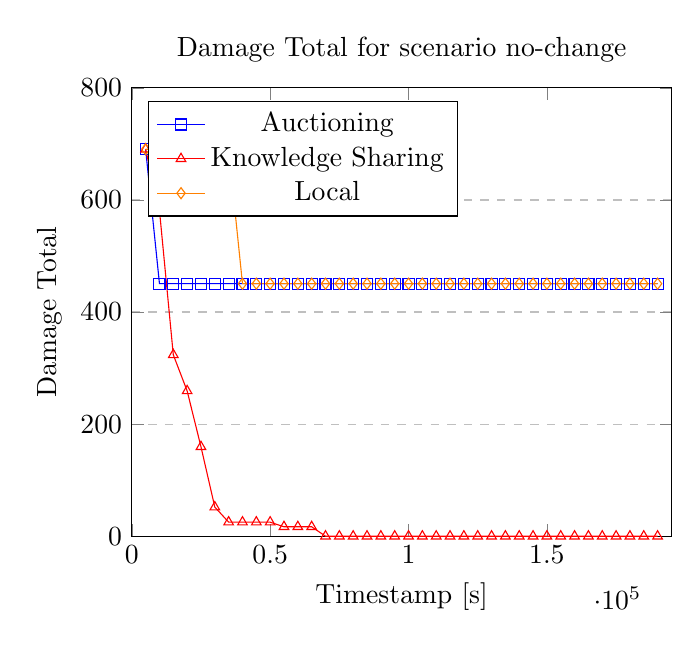
\begin{tikzpicture}
\begin{axis}[
    title={Damage Total for scenario no-change},
    xlabel={Timestamp [s]},
    ylabel={Damage Total},
    xmin=0, xmax=195000,
    ymin=0, ymax=800,
    legend pos=north west,
    ymajorgrids=true,
    grid style=dashed,
]

\addplot[
    color=blue,
    mark=square,
    ]
    coordinates {
    (5000,690.52)(10000,450.57)(15000,450.57)(20000,450.57)(25000,450.57)(30000,450.57)(35000,450.57)(40000,450.57)(45000,450.57)(50000,450.57)(55000,450.57)(60000,450.57)(65000,450.57)(70000,450.57)(75000,450.57)(80000,450.57)(85000,450.57)(90000,450.57)(95000,450.57)(100000,450.57)(105000,450.57)(110000,450.57)(115000,450.57)(120000,450.57)(125000,450.57)(130000,450.57)(135000,450.57)(140000,450.57)(145000,450.57)(150000,450.57)(155000,450.57)(160000,450.57)(165000,450.57)(170000,450.57)(175000,450.57)(180000,450.57)(185000,450.57)(190000,450.57)
    };
    \addlegendentry{Auctioning}
\addplot[
    color=red,
    mark=triangle,
    ]
    coordinates {
    (5000,690.52)(10000,581.45)(15000,323.71)(20000,259.27)(25000,159.58)(30000,51.98)(35000,25.08)(40000,25.08)(45000,25.08)(50000,25.08)(55000,16.82)(60000,16.82)(65000,16.82)(70000,0.00)(75000,0.00)(80000,0.00)(85000,0.00)(90000,0.00)(95000,0.00)(100000,0.00)(105000,0.00)(110000,0.00)(115000,0.00)(120000,0.00)(125000,0.00)(130000,0.00)(135000,0.00)(140000,0.00)(145000,0.00)(150000,0.00)(155000,0.00)(160000,0.00)(165000,0.00)(170000,0.00)(175000,0.00)(180000,0.00)(185000,0.00)(190000,0.00)
    };
    \addlegendentry{Knowledge Sharing}
\addplot[
    color=orange,
    mark=diamond,
    ]
    coordinates {
    (5000,690.52)(10000,690.52)(15000,690.52)(20000,690.52)(25000,690.52)(30000,690.52)(35000,690.52)(40000,450.57)(45000,450.57)(50000,450.57)(55000,450.57)(60000,450.57)(65000,450.57)(70000,450.57)(75000,450.57)(80000,450.57)(85000,450.57)(90000,450.57)(95000,450.57)(100000,450.57)(105000,450.57)(110000,450.57)(115000,450.57)(120000,450.57)(125000,450.57)(130000,450.57)(135000,450.57)(140000,450.57)(145000,450.57)(150000,450.57)(155000,450.57)(160000,450.57)(165000,450.57)(170000,450.57)(175000,450.57)(180000,450.57)(185000,450.57)(190000,450.57)
    };
    \addlegendentry{Local}
    
\end{axis}
\end{tikzpicture}
    \caption{This graph shows the overall damage of the system in the scenario where no changes are made overtime.}
    \label{fig:overall-damage-no-change}
\end{figure}

From figure \ref{fig:overall-damage-no-change} we see that the agent with the Local-feature set (from here-on \textit{local-agent}) slowly reduces the overall damage of the network, but is unable to get any lower than around $275$, and stays at this value after roughly the first $50$ seconds.
Within the first $25$ seconds, the knowledge-sharing agents are able to reduce the overall damage to around $220$, but is unable to get any lower than this. 
Finally, the auctioning are able to reduce the damage to roughly $80$, but is only able to get there after $80$ seconds.
The lowest value is for the auctioning agent at $35\%$ of the damage the local-agent.

\begin{figure}[H]
    \centering
    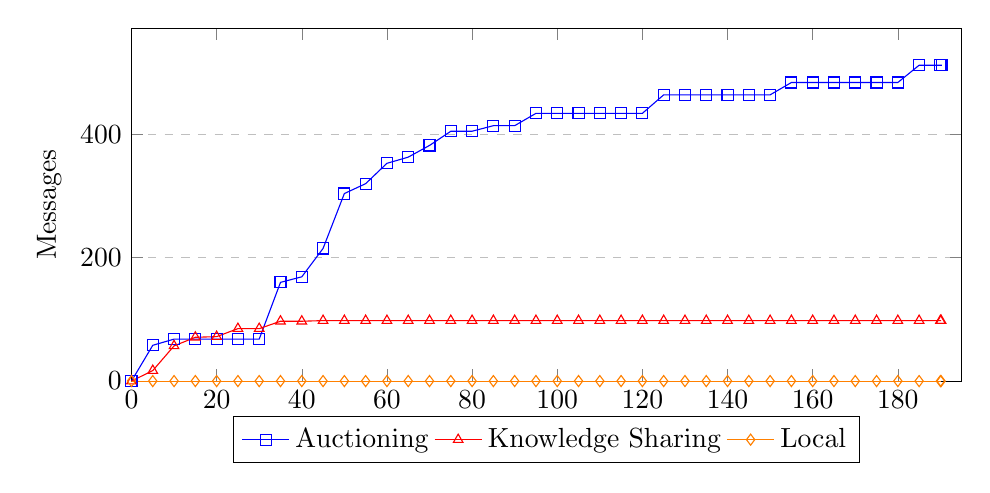
\begin{tikzpicture}
\begin{axis}[
    xlabel={Timestamp [s]},
    ylabel={Messages},
    xmin=0, xmax=195000,
    ymin=0, ymax=572,
    legend columns=-1,
    legend style={at={(0.5,-0.1)},anchor=north},
    ymajorgrids=true,
    grid style=dashed,
    width=\textwidth,
    height=0.5\textwidth,
    scaled x ticks=base 10:-3,
    xtick scale label code/.code={}
]

	\addplot[color=blue,mark=square] coordinates {
        (0,0)(5000,58)(10000,68)(15000,68)(20000,68)(25000,68)(30000,68)(35000,160)(40000,169)(45000,215)(50000,304)(55000,320)(60000,353)(65000,363)(70000,382)(75000,405)(80000,405)(85000,414)(90000,414)(95000,434)(100000,434)(105000,434)(110000,434)(115000,434)(120000,434)(125000,464)(130000,464)(135000,464)(140000,464)(145000,464)(150000,464)(155000,484)(160000,484)(165000,484)(170000,484)(175000,484)(180000,484)(185000,512)(190000,512)(190364,512)
    };
    \addlegendentry{Auctioning}
	\addplot[color=red,mark=triangle] coordinates {
        (0,0)(5000,17)(10000,57)(15000,71)(20000,72)(25000,85)(30000,85)(35000,97)(40000,97)(45000,98)(50000,98)(55000,98)(60000,98)(65000,98)(70000,98)(75000,98)(80000,98)(85000,98)(90000,98)(95000,98)(100000,98)(105000,98)(110000,98)(115000,98)(120000,98)(125000,98)(130000,98)(135000,98)(140000,98)(145000,98)(150000,98)(155000,98)(160000,98)(165000,98)(170000,98)(175000,98)(180000,98)(185000,98)(190000,98)(190165,98)
    };
    \addlegendentry{Knowledge Sharing}
	\addplot[color=orange,mark=diamond] coordinates {
        (0,0)(5000,0)(10000,0)(15000,0)(20000,0)(25000,0)(30000,0)(35000,0)(40000,0)(45000,0)(50000,0)(55000,0)(60000,0)(65000,0)(70000,0)(75000,0)(80000,0)(85000,0)(90000,0)(95000,0)(100000,0)(105000,0)(110000,0)(115000,0)(120000,0)(125000,0)(130000,0)(135000,0)(140000,0)(145000,0)(150000,0)(155000,0)(160000,0)(165000,0)(170000,0)(175000,0)(180000,0)(185000,0)(190000,0)(190150,0)
    };
    \addlegendentry{Local}




\end{axis}
\end{tikzpicture}
    \caption{Graph showing the total amount of messages sent between agents in the scenario where no changes are made overtime.}
    \label{fig:messages-no-change}
\end{figure}

In figure \ref{fig:messages-no-change} we can see that the local-agent shares no messages, as this feature-set does not allow for it. The auctioning agent sends the most messages. After $80$ seconds all agents have found a stable point damage-wise, and this is also visible from the messages for the auctioning agents. At this point the auctioning agents have sent almost three times as much as the knowledge-sharing agents. This can be explained by the fact that the auctioning agents have a total of $11$ events that can be sent to other agents, compared to the knowledge-sharing agent, which has only $4$ types of messages. This $4 / 11$ ratio is roughly the same as the ratio between the amount of messages sent by the auctioning and knowledge-sharing agents. However, this could be a coincidence, and more research would be needed for this assumption. During an auction participating nodes send on average $4$ messages per participating node, which could also explain the difference in messages sent. 

The message count for auctioning nodes goes up roughly every $30$ second, which is the interval at which any agent will start identifying risks if it has received no messages. During this time the agents share some knowledge, sometimes try an auction but then stop because there are no proposals to be made.

\begin{figure}[H]
    \centering
    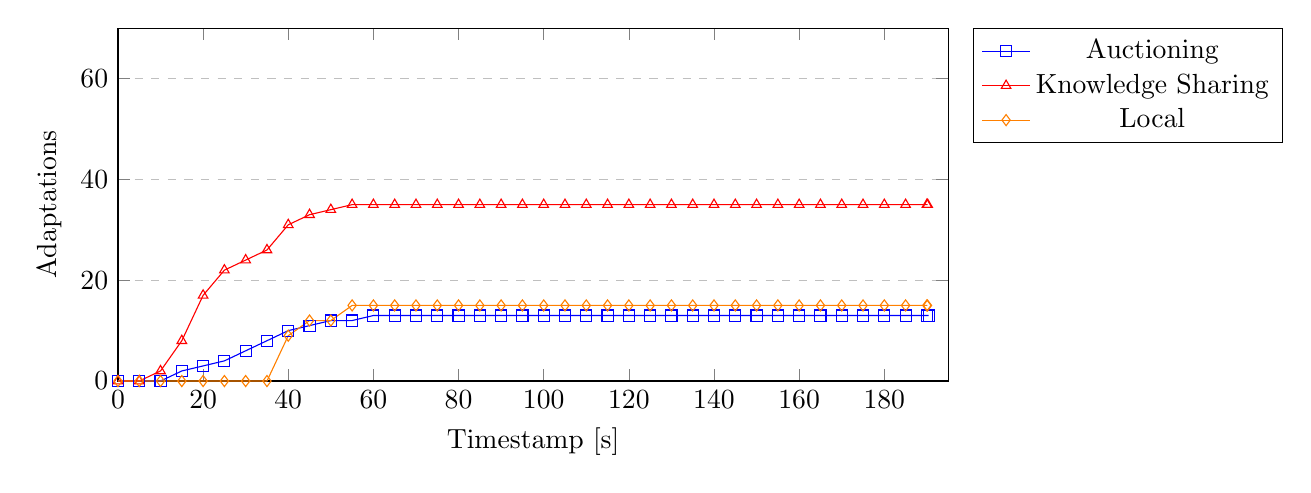
\begin{tikzpicture}
\begin{axis}[
    xlabel={Timestamp [s]},
    ylabel={Adaptations},
    xmin=0, xmax=195000,
    ymin=0, ymax=70,
    legend pos=outer north east,
    ymajorgrids=true,
    grid style=dashed,
    width=\textwidth,
    height=0.5\textwidth,
    scaled x ticks=base 10:-3,
    xtick scale label code/.code={}
]

	\addplot[color=blue,mark=square] coordinates {
        (0,0)(5000,0)(10000,0)(15000,2)(20000,3)(25000,4)(30000,6)(35000,8)(40000,10)(45000,11)(50000,12)(55000,12)(60000,13)(65000,13)(70000,13)(75000,13)(80000,13)(85000,13)(90000,13)(95000,13)(100000,13)(105000,13)(110000,13)(115000,13)(120000,13)(125000,13)(130000,13)(135000,13)(140000,13)(145000,13)(150000,13)(155000,13)(160000,13)(165000,13)(170000,13)(175000,13)(180000,13)(185000,13)(190000,13)(190434,13)
    };
    \addlegendentry{Auctioning}
	\addplot[color=red,mark=triangle] coordinates {
        (0,0)(5000,0)(10000,2)(15000,8)(20000,17)(25000,22)(30000,24)(35000,26)(40000,31)(45000,33)(50000,34)(55000,35)(60000,35)(65000,35)(70000,35)(75000,35)(80000,35)(85000,35)(90000,35)(95000,35)(100000,35)(105000,35)(110000,35)(115000,35)(120000,35)(125000,35)(130000,35)(135000,35)(140000,35)(145000,35)(150000,35)(155000,35)(160000,35)(165000,35)(170000,35)(175000,35)(180000,35)(185000,35)(190000,35)(190190,35)
    };
    \addlegendentry{Knowledge Sharing}
	\addplot[color=orange,mark=diamond] coordinates {
        (0,0)(5000,0)(10000,0)(15000,0)(20000,0)(25000,0)(30000,0)(35000,0)(40000,9)(45000,12)(50000,12)(55000,15)(60000,15)(65000,15)(70000,15)(75000,15)(80000,15)(85000,15)(90000,15)(95000,15)(100000,15)(105000,15)(110000,15)(115000,15)(120000,15)(125000,15)(130000,15)(135000,15)(140000,15)(145000,15)(150000,15)(155000,15)(160000,15)(165000,15)(170000,15)(175000,15)(180000,15)(185000,15)(190000,15)(190138,15)
    };
    \addlegendentry{Local}




\end{axis}
\end{tikzpicture}
    \caption{Graph showing the total amount of adaptations applied by agents in the scenario where no changes are made overtime.}
    \label{fig:proposals-no-change}
\end{figure}

From figure \ref{fig:proposals-no-change} we can see that the knowledge-sharing agent applies the most adaptations, followed by the auctioning agent. The local-agent applies the least adaptations. The knowledge-sharing agent applies almost $3$ times  more adaptations than the local agent. The knowledge-sharing agent has a steep increase in the first $25$ seconds, after which it becomes more stable. The auctioning agent has a slower increase, but is applying adaptations at a steady rate. This is to be expected as any adaptation will be negotiated first, which takes time.

\begin{figure}[H]
    \centering
        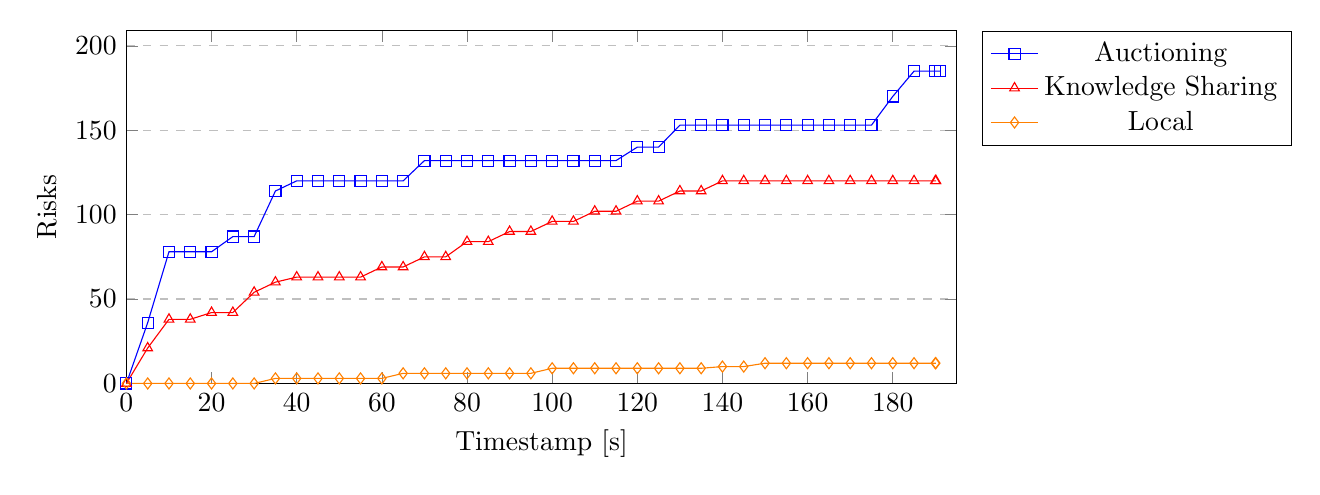
\begin{tikzpicture}
\begin{axis}[
    xlabel={Timestamp [s]},
    ylabel={Risks},
    xmin=0, xmax=195000,
    ymin=0, ymax=209,
    legend pos=outer north east,
    ymajorgrids=true,
    grid style=dashed,
    width=\textwidth,
    height=0.5\textwidth,
    scaled x ticks=base 10:-3,
    xtick scale label code/.code={}
]

	\addplot[color=blue,mark=square] coordinates {
        (0,0)(5000,36)(10000,78)(15000,78)(20000,78)(25000,87)(30000,87)(35000,114)(40000,120)(45000,120)(50000,120)(55000,120)(60000,120)(65000,120)(70000,132)(75000,132)(80000,132)(85000,132)(90000,132)(95000,132)(100000,132)(105000,132)(110000,132)(115000,132)(120000,140)(125000,140)(130000,153)(135000,153)(140000,153)(145000,153)(150000,153)(155000,153)(160000,153)(165000,153)(170000,153)(175000,153)(180000,170)(185000,185)(190000,185)(191066,185)
    };
    \addlegendentry{Auctioning}
	\addplot[color=red,mark=triangle] coordinates {
        (0,0)(5000,21)(10000,38)(15000,38)(20000,42)(25000,42)(30000,54)(35000,60)(40000,63)(45000,63)(50000,63)(55000,63)(60000,69)(65000,69)(70000,75)(75000,75)(80000,84)(85000,84)(90000,90)(95000,90)(100000,96)(105000,96)(110000,102)(115000,102)(120000,108)(125000,108)(130000,114)(135000,114)(140000,120)(145000,120)(150000,120)(155000,120)(160000,120)(165000,120)(170000,120)(175000,120)(180000,120)(185000,120)(190000,120)(190155,120)
    };
    \addlegendentry{Knowledge Sharing}
	\addplot[color=orange,mark=diamond] coordinates {
        (0,0)(5000,0)(10000,0)(15000,0)(20000,0)(25000,0)(30000,0)(35000,3)(40000,3)(45000,3)(50000,3)(55000,3)(60000,3)(65000,6)(70000,6)(75000,6)(80000,6)(85000,6)(90000,6)(95000,6)(100000,9)(105000,9)(110000,9)(115000,9)(120000,9)(125000,9)(130000,9)(135000,9)(140000,10)(145000,10)(150000,12)(155000,12)(160000,12)(165000,12)(170000,12)(175000,12)(180000,12)(185000,12)(190000,12)(190110,12)
    };
    \addlegendentry{Local}




\end{axis}
\end{tikzpicture}
    \caption{Graph showing the number of unique risks detected by agents in the scenario where no changes are made overtime.}
    \label{fig:risk-count-no-change}
\end{figure}

Figure \ref{fig:risk-count-no-change} shows that the knowledge-sharing agent detects the most risks, followed by the auctioning agent with roughly $70\%$ of the risks found. The local-agent detects the least amount of risks at only $10\%$ compared to the auctioning agent. It is to be expected that the local-agents can only detect a fraction of what the other agents detect, as the risks that can be deduced from only their local knowledge is limited.

\begin{figure}[H]
    \centering
        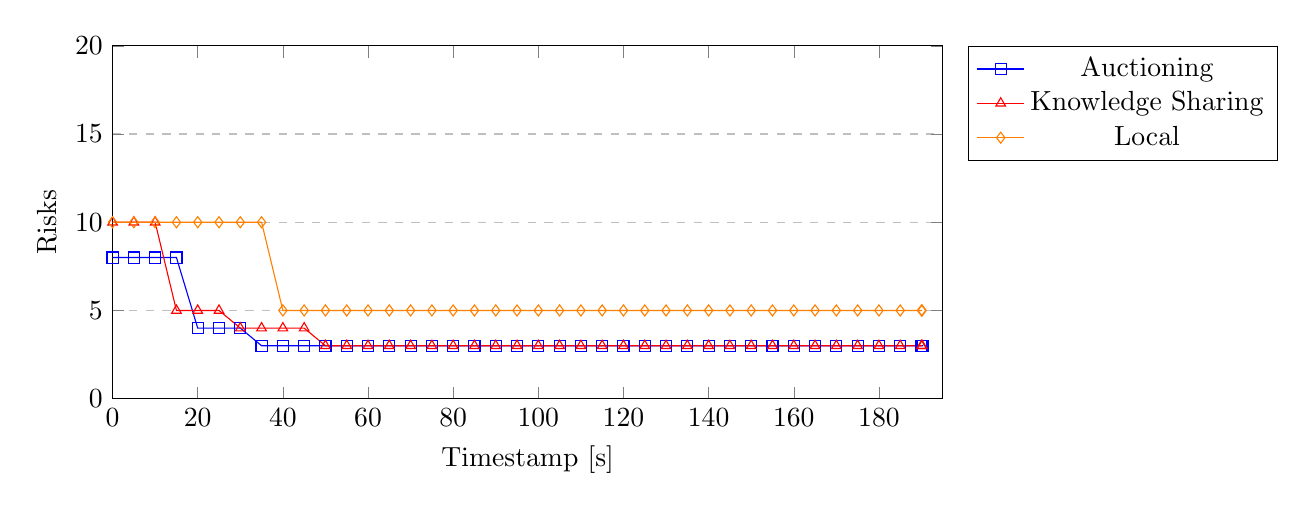
\begin{tikzpicture}
\begin{axis}[
    xlabel={Timestamp [s]},
    ylabel={Risks},
    xmin=0, xmax=195000,
    ymin=0, ymax=20,
    legend pos=outer north east,
    ymajorgrids=true,
    grid style=dashed,
    width=\textwidth,
    height=0.5\textwidth,
    scaled x ticks=base 10:-3,
    xtick scale label code/.code={}
]

	\addplot[color=blue,mark=square] coordinates {
        (0,8)(5000,8)(10000,8)(15000,8)(20000,4)(25000,4)(30000,4)(35000,3)(40000,3)(45000,3)(50000,3)(55000,3)(60000,3)(65000,3)(70000,3)(75000,3)(80000,3)(85000,3)(90000,3)(95000,3)(100000,3)(105000,3)(110000,3)(115000,3)(120000,3)(125000,3)(130000,3)(135000,3)(140000,3)(145000,3)(150000,3)(155000,3)(160000,3)(165000,3)(170000,3)(175000,3)(180000,3)(185000,3)(190000,3)(190439,3)
    };
    \addlegendentry{Auctioning}
	\addplot[color=red,mark=triangle] coordinates {
        (0,10)(5000,10)(10000,10)(15000,5)(20000,5)(25000,5)(30000,4)(35000,4)(40000,4)(45000,4)(50000,3)(55000,3)(60000,3)(65000,3)(70000,3)(75000,3)(80000,3)(85000,3)(90000,3)(95000,3)(100000,3)(105000,3)(110000,3)(115000,3)(120000,3)(125000,3)(130000,3)(135000,3)(140000,3)(145000,3)(150000,3)(155000,3)(160000,3)(165000,3)(170000,3)(175000,3)(180000,3)(185000,3)(190000,3)(190147,3)
    };
    \addlegendentry{Knowledge Sharing}
	\addplot[color=orange,mark=diamond] coordinates {
        (0,10)(5000,10)(10000,10)(15000,10)(20000,10)(25000,10)(30000,10)(35000,10)(40000,5)(45000,5)(50000,5)(55000,5)(60000,5)(65000,5)(70000,5)(75000,5)(80000,5)(85000,5)(90000,5)(95000,5)(100000,5)(105000,5)(110000,5)(115000,5)(120000,5)(125000,5)(130000,5)(135000,5)(140000,5)(145000,5)(150000,5)(155000,5)(160000,5)(165000,5)(170000,5)(175000,5)(180000,5)(185000,5)(190000,5)(190136,5)
    };
    \addlegendentry{Local}




\end{axis}
\end{tikzpicture}
    \caption{Graph showing the number of remaining risks in the infrastructure in the scenario where no changes are made overtime.}
    \label{fig:risk-remaining-no-change}
\end{figure}

When comparing figure \ref{fig:overall-damage-no-change} to figure \ref{fig:risk-remaining-no-change}, we see that the graphs are following the same trend. This is to be expected, as the overall damage is calculated by summing the damage of all the remaining risks.

\begin{figure}[H]
    \centering
        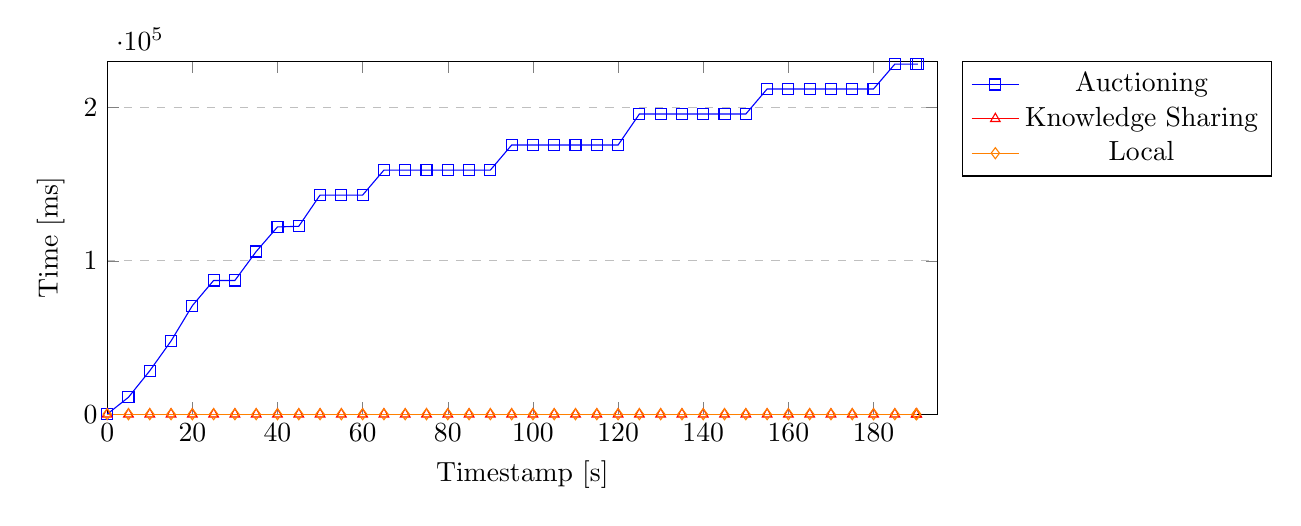
\begin{tikzpicture}
\begin{axis}[
    xlabel={Timestamp [s]},
    ylabel={Time [ms]},
    xmin=0, xmax=195000,
    ymin=0, ymax=230023,
    legend pos=outer north east,
    ymajorgrids=true,
    grid style=dashed,
    width=\textwidth,
    height=0.5\textwidth,
    scaled x ticks=base 10:-3,
    xtick scale label code/.code={}
]

	\addplot[color=blue,mark=square] coordinates {
        (0,0)(5000,11025)(10000,28282)(15000,47709)(20000,70713)(25000,87182)(30000,87182)(35000,106048)(40000,122066)(45000,122489)(50000,142841)(55000,142841)(60000,142841)(65000,159124)(70000,159124)(75000,159124)(80000,159124)(85000,159124)(90000,159124)(95000,175471)(100000,175471)(105000,175471)(110000,175471)(115000,175471)(120000,175471)(125000,195658)(130000,195658)(135000,195658)(140000,195658)(145000,195658)(150000,195658)(155000,212013)(160000,212013)(165000,212013)(170000,212013)(175000,212013)(180000,212013)(185000,228231)(190000,228231)(190439,228231)
    };
    \addlegendentry{Auctioning}
	\addplot[color=red,mark=triangle] coordinates {
        (0,0)(5000,0)(10000,0)(15000,0)(20000,0)(25000,0)(30000,0)(35000,0)(40000,0)(45000,0)(50000,0)(55000,0)(60000,0)(65000,0)(70000,0)(75000,0)(80000,0)(85000,0)(90000,0)(95000,0)(100000,0)(105000,0)(110000,0)(115000,0)(120000,0)(125000,0)(130000,0)(135000,0)(140000,0)(145000,0)(150000,0)(155000,0)(160000,0)(165000,0)(170000,0)(175000,0)(180000,0)(185000,0)(190000,0)(190147,0)
    };
    \addlegendentry{Knowledge Sharing}
	\addplot[color=orange,mark=diamond] coordinates {
        (0,0)(5000,0)(10000,0)(15000,0)(20000,0)(25000,0)(30000,0)(35000,0)(40000,0)(45000,0)(50000,0)(55000,0)(60000,0)(65000,0)(70000,0)(75000,0)(80000,0)(85000,0)(90000,0)(95000,0)(100000,0)(105000,0)(110000,0)(115000,0)(120000,0)(125000,0)(130000,0)(135000,0)(140000,0)(145000,0)(150000,0)(155000,0)(160000,0)(165000,0)(170000,0)(175000,0)(180000,0)(185000,0)(190000,0)(190136,0)
    };
    \addlegendentry{Local}




\end{axis}
\end{tikzpicture}
    \caption{Graph showing the sum of time spent auctioning by agents in the scenario where no changes are made overtime.}
    \label{fig:auctioning-time-no-change}
\end{figure}

Figure \ref{fig:auctioning-time-no-change} shows that the auctioning agents is the only agent that spends time auctioning. This is to be expected, as the auctioning agents are the only agents that can auction.

\begin{figure}[H]
    \centering
        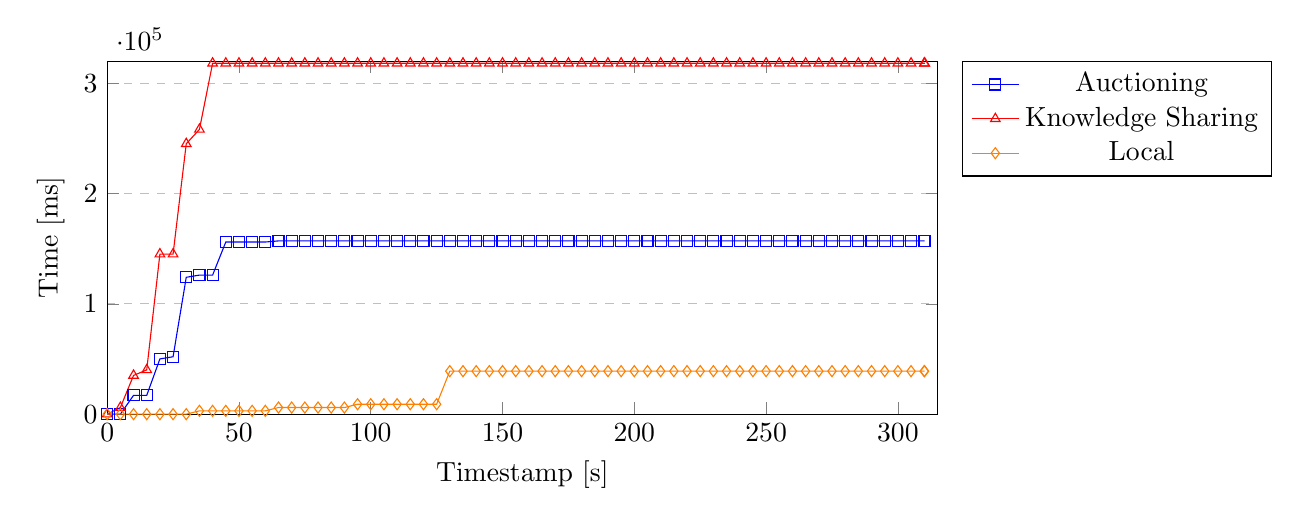
\begin{tikzpicture}
\begin{axis}[
    xlabel={Timestamp [s]},
    ylabel={Time [ms]},
    xmin=0, xmax=315000,
    ymin=0, ymax=320032,
    legend pos=outer north east,
    ymajorgrids=true,
    grid style=dashed,
    width=\textwidth,
    height=0.5\textwidth,
    scaled x ticks=base 10:-3,
    xtick scale label code/.code={}
]

	\addplot[color=blue,mark=square] coordinates {
        (0,0)(5000,0)(10000,17072)(15000,17072)(20000,50094)(25000,52106)(30000,124138)(35000,126144)(40000,126144)(45000,156154)(50000,156154)(55000,156154)(60000,156154)(65000,157158)(70000,157158)(75000,157158)(80000,157158)(85000,157158)(90000,157158)(95000,157158)(100000,157158)(105000,157158)(110000,157158)(115000,157158)(120000,157158)(125000,157158)(130000,157158)(135000,157158)(140000,157158)(145000,157158)(150000,157158)(155000,157158)(160000,157158)(165000,157158)(170000,157158)(175000,157158)(180000,157158)(185000,157158)(190000,157158)(195000,157158)(200000,157158)(205000,157158)(210000,157158)(215000,157158)(220000,157158)(225000,157158)(230000,157158)(235000,157158)(240000,157158)(245000,157158)(250000,157158)(255000,157158)(260000,157158)(265000,157158)(270000,157158)(275000,157158)(280000,157158)(285000,157158)(290000,157158)(295000,157158)(300000,157158)(305000,157158)(310000,157158)(310159,157158)
    };
    \addlegendentry{Auctioning}
	\addplot[color=red,mark=triangle] coordinates {
        (0,0)(5000,6039)(10000,35135)(15000,40149)(20000,145217)(25000,145217)(30000,245261)(35000,258272)(40000,318293)(45000,318293)(50000,318293)(55000,318293)(60000,318293)(65000,318293)(70000,318293)(75000,318293)(80000,318293)(85000,318293)(90000,318293)(95000,318293)(100000,318293)(105000,318293)(110000,318293)(115000,318293)(120000,318293)(125000,318293)(130000,318293)(135000,318293)(140000,318293)(145000,318293)(150000,318293)(155000,318293)(160000,318293)(165000,318293)(170000,318293)(175000,318293)(180000,318293)(185000,318293)(190000,318293)(195000,318293)(200000,318293)(205000,318293)(210000,318293)(215000,318293)(220000,318293)(225000,318293)(230000,318293)(235000,318293)(240000,318293)(245000,318293)(250000,318293)(255000,318293)(260000,318293)(265000,318293)(270000,318293)(275000,318293)(280000,318293)(285000,318293)(290000,318293)(295000,318293)(300000,318293)(305000,318293)(310000,318293)(310212,318293)
    };
    \addlegendentry{Knowledge Sharing}
	\addplot[color=orange,mark=diamond] coordinates {
        (0,0)(5000,0)(10000,0)(15000,0)(20000,0)(25000,0)(30000,0)(35000,3012)(40000,3012)(45000,3012)(50000,3012)(55000,3012)(60000,3012)(65000,6020)(70000,6020)(75000,6020)(80000,6020)(85000,6020)(90000,6020)(95000,9026)(100000,9026)(105000,9026)(110000,9026)(115000,9026)(120000,9026)(125000,9026)(130000,39035)(135000,39035)(140000,39035)(145000,39035)(150000,39035)(155000,39035)(160000,39035)(165000,39035)(170000,39035)(175000,39035)(180000,39035)(185000,39035)(190000,39035)(195000,39035)(200000,39035)(205000,39035)(210000,39035)(215000,39035)(220000,39035)(225000,39035)(230000,39035)(235000,39035)(240000,39035)(245000,39035)(250000,39035)(255000,39035)(260000,39035)(265000,39035)(270000,39035)(275000,39035)(280000,39035)(285000,39035)(290000,39035)(295000,39035)(300000,39035)(305000,39035)(310000,39035)(310137,39035)
    };
    \addlegendentry{Local}




\end{axis}
\end{tikzpicture}
    \caption{Graph showing the sum of time spent adapting by agents in the scenario where no changes are made overtime.}
    \label{fig:adapting-time-no-change}
\end{figure}

Figure \ref{fig:adapting-time-no-change} shows that the knowledge-sharing agents spends the most amount of time adapting during this scenario. The auctioning agent is second, and the local agent spends the least amount of time adapting. This is inline with the amount of adaptations applied.

\subsection{Scenario 2: Risk Introduction}
\label{ssec:scenario-2-results}
\textit{This scenario introduces a risk to the infrastructure after $180$ seconds. The purpose of this scenario is to see how the system behaves when a new risk is introduced.}

\begin{figure}[H]
    \centering
    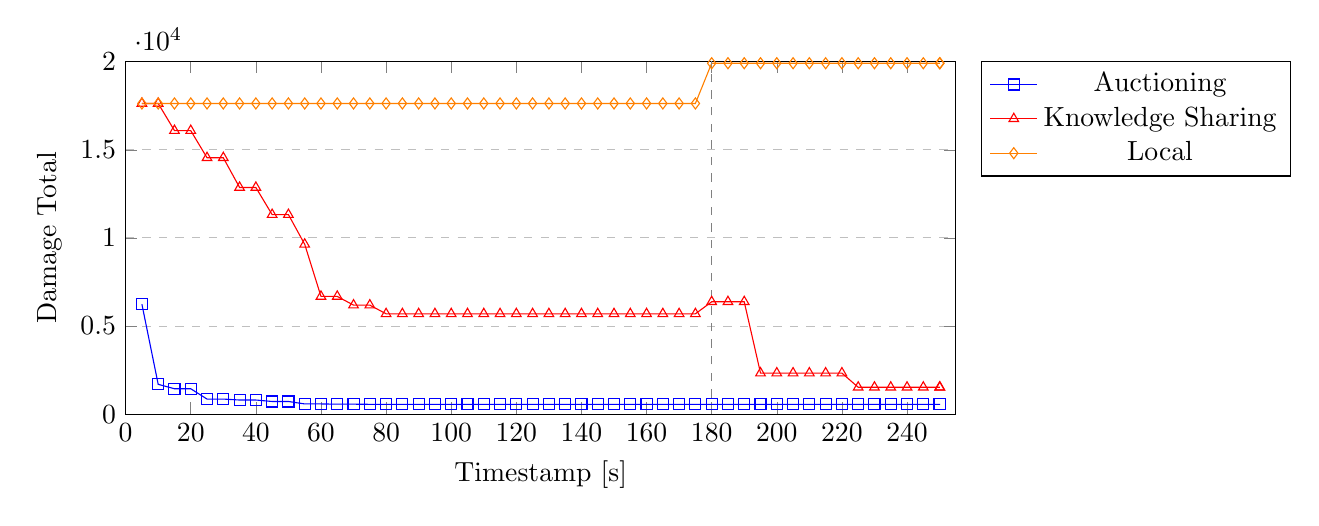
\begin{tikzpicture}
\begin{axis}[
    xlabel={Timestamp [s]},
    ylabel={Damage Total},
    xmin=0, xmax=255000,
    ymin=0, ymax=20020,
    legend pos=outer north east,
    ymajorgrids=true,
    grid style=dashed,
    width=\textwidth,
    height=0.5\textwidth,
    scaled x ticks=base 10:-3,
    xtick scale label code/.code={}
]

	\addplot[color=blue,mark=square] coordinates {
        (5000,6236.51)(10000,1693.70)(15000,1442.78)(20000,1442.78)(25000,857.00)(30000,857.00)(35000,803.10)(40000,803.10)(45000,720.33)(50000,720.33)(55000,580.88)(60000,580.88)(65000,567.64)(70000,567.64)(75000,559.15)(80000,556.95)(85000,556.95)(90000,556.95)(95000,556.95)(100000,556.95)(105000,556.95)(110000,556.95)(115000,556.95)(120000,556.95)(125000,556.95)(130000,556.95)(135000,556.95)(140000,556.95)(145000,556.95)(150000,556.95)(155000,556.95)(160000,556.95)(165000,556.95)(170000,556.95)(175000,556.95)(180000,556.95)(185000,560.22)(190000,560.22)(195000,560.22)(200000,560.22)(205000,560.22)(210000,560.22)(215000,560.22)(220000,560.22)(225000,560.22)(230000,560.22)(235000,560.22)(240000,560.22)(245000,560.22)(250000,560.22)(250139,560.22)
    };
    \addlegendentry{Auctioning}
	\addplot[color=red,mark=triangle] coordinates {
        (5000,17629.95)(10000,17629.95)(15000,16089.24)(20000,16089.24)(25000,14548.54)(30000,14548.54)(35000,12864.04)(40000,12864.04)(45000,11323.33)(50000,11323.33)(55000,9638.83)(60000,6680.68)(65000,6680.68)(70000,6187.65)(75000,6187.65)(80000,5694.63)(85000,5694.63)(90000,5694.63)(95000,5694.63)(100000,5694.63)(105000,5694.63)(110000,5694.63)(115000,5694.63)(120000,5694.63)(125000,5694.63)(130000,5694.63)(135000,5694.63)(140000,5694.63)(145000,5694.63)(150000,5694.63)(155000,5694.63)(160000,5694.63)(165000,5694.63)(170000,5694.63)(175000,5694.63)(180000,6377.52)(185000,6377.52)(190000,6377.52)(195000,2331.23)(200000,2331.23)(205000,2331.23)(210000,2331.23)(215000,2331.23)(220000,2331.23)(225000,1526.78)(230000,1526.78)(235000,1526.78)(240000,1526.78)(245000,1526.78)(250000,1526.78)(250111,1526.78)
    };
    \addlegendentry{Knowledge Sharing}
	\addplot[color=orange,mark=diamond] coordinates {
        (5000,17629.95)(10000,17629.95)(15000,17629.95)(20000,17629.95)(25000,17629.95)(30000,17629.95)(35000,17629.95)(40000,17629.95)(45000,17629.95)(50000,17629.95)(55000,17629.95)(60000,17629.95)(65000,17629.95)(70000,17629.95)(75000,17629.95)(80000,17629.95)(85000,17629.95)(90000,17629.95)(95000,17629.95)(100000,17629.95)(105000,17629.95)(110000,17629.95)(115000,17629.95)(120000,17629.95)(125000,17629.95)(130000,17629.95)(135000,17629.95)(140000,17629.95)(145000,17629.95)(150000,17629.95)(155000,17629.95)(160000,17629.95)(165000,17629.95)(170000,17629.95)(175000,17629.95)(180000,19913.02)(185000,19913.02)(190000,19913.02)(195000,19913.02)(200000,19913.02)(205000,19913.02)(210000,19913.02)(215000,19913.02)(220000,19913.02)(225000,19913.02)(230000,19913.02)(235000,19913.02)(240000,19913.02)(245000,19913.02)(250000,19913.02)(250115,19913.02)
    };
    \addlegendentry{Local}

	\addplot[color=gray, dashed,] coordinates {(180000,0) (180000,20020)};


\end{axis}
\end{tikzpicture}
    \caption{This graph shows the overall damage of the system in the risk introduction scenario. The damage is shown for each of the three strategies. The vertical lines indicate the time at which a risk is introduced.}
    \label{fig:overall-damage-inroduce-risk}
\end{figure}

Figure \ref{fig:overall-damage-inroduce-risk} shows a graph that follows a similar trend as shown in figure \ref{fig:overall-damage-no-change}, albeit a bit slower for the auctioning agent. This is to be expected as the scenarios are identical up until the $120$ seconds mark. During this time we see a small increase in damage for all graphs. As the metrics are collected in $5000$ms intervals, we see a small bump in all the lines around the $120$ seconds mark. And it slowly goes down again after this. Due to this timing, agents sometimes applied the adaptation before the interval ended. This explains why sometimes the lines are not as smooth as we would expect.

\begin{figure}[H]
    \centering
    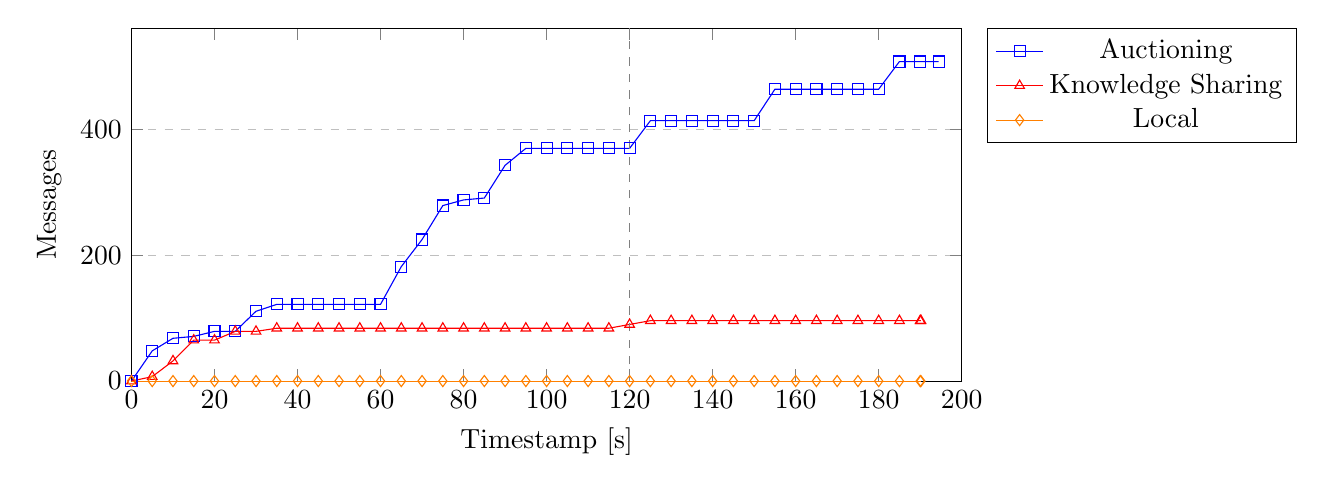
\begin{tikzpicture}
\begin{axis}[
    xlabel={Timestamp [s]},
    ylabel={Messages},
    xmin=0, xmax=200000,
    ymin=0, ymax=561,
    legend pos=outer north east,
    ymajorgrids=true,
    grid style=dashed,
    width=\textwidth,
    height=0.5\textwidth,
    scaled x ticks=base 10:-3,
    xtick scale label code/.code={}
]

	\addplot[color=blue,mark=square] coordinates {
        (0,0)(5000,48)(10000,68)(15000,71)(20000,79)(25000,79)(30000,111)(35000,122)(40000,122)(45000,122)(50000,122)(55000,122)(60000,122)(65000,182)(70000,225)(75000,279)(80000,288)(85000,291)(90000,343)(95000,370)(100000,370)(105000,370)(110000,370)(115000,370)(120000,370)(125000,414)(130000,414)(135000,414)(140000,414)(145000,414)(150000,414)(155000,464)(160000,464)(165000,464)(170000,464)(175000,464)(180000,464)(185000,508)(190000,508)(194440,508)
    };
    \addlegendentry{Auctioning}
	\addplot[color=red,mark=triangle] coordinates {
        (0,0)(5000,7)(10000,32)(15000,65)(20000,65)(25000,79)(30000,79)(35000,84)(40000,84)(45000,84)(50000,84)(55000,84)(60000,84)(65000,84)(70000,84)(75000,84)(80000,84)(85000,84)(90000,84)(95000,84)(100000,84)(105000,84)(110000,84)(115000,84)(120000,90)(125000,96)(130000,96)(135000,96)(140000,96)(145000,96)(150000,96)(155000,96)(160000,96)(165000,96)(170000,96)(175000,96)(180000,96)(185000,96)(190000,96)(190192,96)
    };
    \addlegendentry{Knowledge Sharing}
	\addplot[color=orange,mark=diamond] coordinates {
        (0,0)(5000,0)(10000,0)(15000,0)(20000,0)(25000,0)(30000,0)(35000,0)(40000,0)(45000,0)(50000,0)(55000,0)(60000,0)(65000,0)(70000,0)(75000,0)(80000,0)(85000,0)(90000,0)(95000,0)(100000,0)(105000,0)(110000,0)(115000,0)(120000,0)(125000,0)(130000,0)(135000,0)(140000,0)(145000,0)(150000,0)(155000,0)(160000,0)(165000,0)(170000,0)(175000,0)(180000,0)(185000,0)(190000,0)(190162,0)
    };
    \addlegendentry{Local}

	\addplot[color=gray, dashed,] coordinates {(120000,0) (120000,561)};


\end{axis}
\end{tikzpicture}
    \caption{Graph showing the total amount of messages sent between agents in the risk introduction scenario.}
    \label{fig:messages-risk-introduction}
\end{figure}

Figure \ref{fig:messages-risk-introduction} shows a graph similar to figure \ref{fig:messages-no-change}. The auctioning agent sends the most messages, followed by the knowledge-sharing agent. The local-agent sends no messages. We see that after the $120$ seconds mark, both the auctioning and knowledge-sharing agents send a few more messages around. This is to be expected as the agents detect a change in their properties, and start sharing this information with other agents.

\begin{figure}[H]
    \centering
    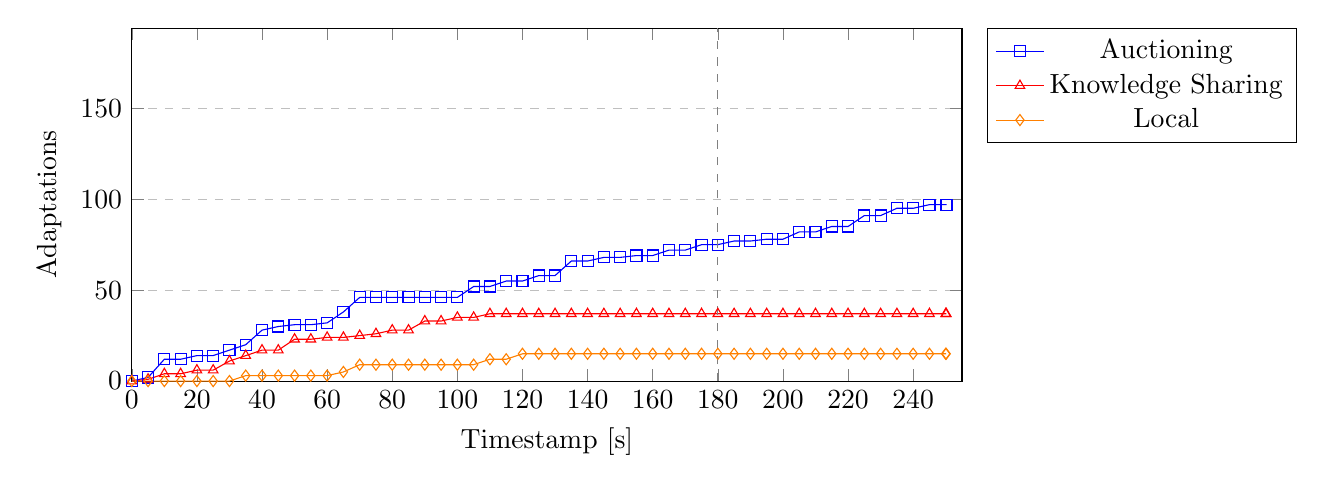
\begin{tikzpicture}
\begin{axis}[
    xlabel={Timestamp [s]},
    ylabel={Adaptations},
    xmin=0, xmax=255000,
    ymin=0, ymax=194,
    legend pos=outer north east,
    ymajorgrids=true,
    grid style=dashed,
    width=\textwidth,
    height=0.5\textwidth,
    scaled x ticks=base 10:-3,
    xtick scale label code/.code={}
]

	\addplot[color=blue,mark=square] coordinates {
        (0,0)(5000,2)(10000,12)(15000,12)(20000,14)(25000,14)(30000,17)(35000,20)(40000,28)(45000,30)(50000,31)(55000,31)(60000,32)(65000,38)(70000,46)(75000,46)(80000,46)(85000,46)(90000,46)(95000,46)(100000,46)(105000,52)(110000,52)(115000,55)(120000,55)(125000,58)(130000,58)(135000,66)(140000,66)(145000,68)(150000,68)(155000,69)(160000,69)(165000,72)(170000,72)(175000,75)(180000,75)(185000,77)(190000,77)(195000,78)(200000,78)(205000,82)(210000,82)(215000,85)(220000,85)(225000,91)(230000,91)(235000,95)(240000,95)(245000,97)(250000,97)(250288,97)
    };
    \addlegendentry{Auctioning}
	\addplot[color=red,mark=triangle] coordinates {
        (0,0)(5000,1)(10000,4)(15000,4)(20000,6)(25000,6)(30000,11)(35000,14)(40000,17)(45000,17)(50000,23)(55000,23)(60000,24)(65000,24)(70000,25)(75000,26)(80000,28)(85000,28)(90000,33)(95000,33)(100000,35)(105000,35)(110000,37)(115000,37)(120000,37)(125000,37)(130000,37)(135000,37)(140000,37)(145000,37)(150000,37)(155000,37)(160000,37)(165000,37)(170000,37)(175000,37)(180000,37)(185000,37)(190000,37)(195000,37)(200000,37)(205000,37)(210000,37)(215000,37)(220000,37)(225000,37)(230000,37)(235000,37)(240000,37)(245000,37)(250000,37)(250159,37)
    };
    \addlegendentry{Knowledge Sharing}
	\addplot[color=orange,mark=diamond] coordinates {
        (0,0)(5000,0)(10000,0)(15000,0)(20000,0)(25000,0)(30000,0)(35000,3)(40000,3)(45000,3)(50000,3)(55000,3)(60000,3)(65000,5)(70000,9)(75000,9)(80000,9)(85000,9)(90000,9)(95000,9)(100000,9)(105000,9)(110000,12)(115000,12)(120000,15)(125000,15)(130000,15)(135000,15)(140000,15)(145000,15)(150000,15)(155000,15)(160000,15)(165000,15)(170000,15)(175000,15)(180000,15)(185000,15)(190000,15)(195000,15)(200000,15)(205000,15)(210000,15)(215000,15)(220000,15)(225000,15)(230000,15)(235000,15)(240000,15)(245000,15)(250000,15)(250135,15)
    };
    \addlegendentry{Local}

	\addplot[color=gray, dashed,] coordinates {(180000,0) (180000,194)};


\end{axis}
\end{tikzpicture}
    \caption{Graph showing the total amount of adaptations applied by agents in the risk introduction scenario.}
    \label{fig:proposals-risk-introduction}
\end{figure}

When the risk is introduced after $120$ seconds, we can see in Figure \ref{fig:proposals-risk-introduction} that a few new adaptations are applied. This is in line with the damage graph in figure \ref{fig:overall-damage-inroduce-risk}.

\begin{figure}[H]
    \centering
        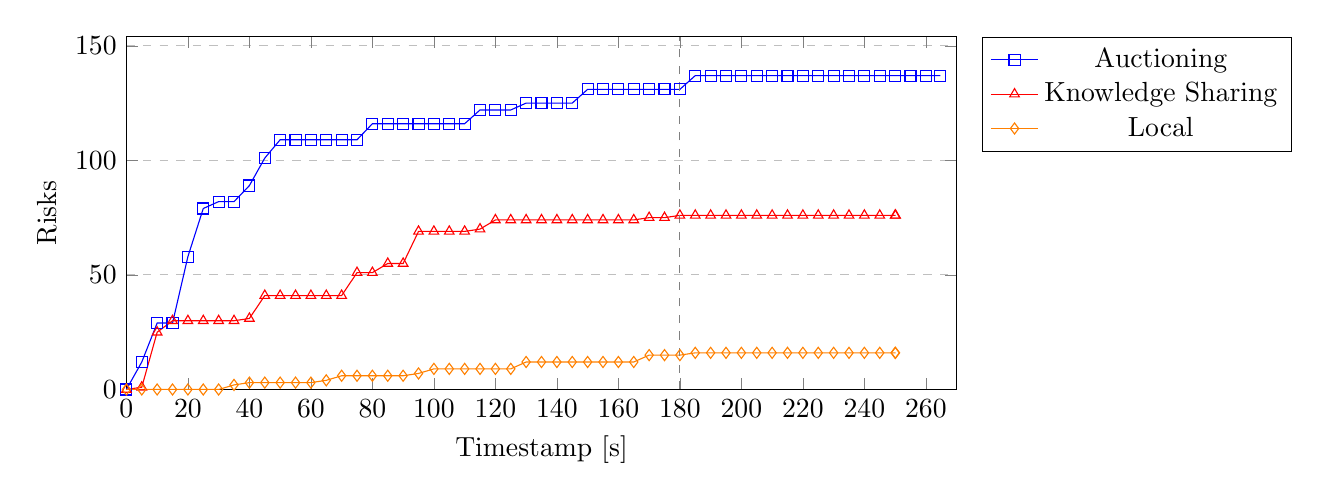
\begin{tikzpicture}
\begin{axis}[
    xlabel={Timestamp [s]},
    ylabel={Risks},
    xmin=0, xmax=270000,
    ymin=0, ymax=154,
    legend pos=outer north east,
    ymajorgrids=true,
    grid style=dashed,
    width=\textwidth,
    height=0.5\textwidth,
    scaled x ticks=base 10:-3,
    xtick scale label code/.code={}
]

	\addplot[color=blue,mark=square] coordinates {
        (0,0)(5000,12)(10000,29)(15000,29)(20000,58)(25000,79)(30000,82)(35000,82)(40000,89)(45000,101)(50000,109)(55000,109)(60000,109)(65000,109)(70000,109)(75000,109)(80000,116)(85000,116)(90000,116)(95000,116)(100000,116)(105000,116)(110000,116)(115000,122)(120000,122)(125000,122)(130000,125)(135000,125)(140000,125)(145000,125)(150000,131)(155000,131)(160000,131)(165000,131)(170000,131)(175000,131)(180000,131)(185000,137)(190000,137)(195000,137)(200000,137)(205000,137)(210000,137)(215000,137)(220000,137)(225000,137)(230000,137)(235000,137)(240000,137)(245000,137)(250000,137)(255000,137)(260000,137)(264723,137)
    };
    \addlegendentry{Auctioning}
	\addplot[color=red,mark=triangle] coordinates {
        (0,0)(5000,1)(10000,25)(15000,30)(20000,30)(25000,30)(30000,30)(35000,30)(40000,31)(45000,41)(50000,41)(55000,41)(60000,41)(65000,41)(70000,41)(75000,51)(80000,51)(85000,55)(90000,55)(95000,69)(100000,69)(105000,69)(110000,69)(115000,70)(120000,74)(125000,74)(130000,74)(135000,74)(140000,74)(145000,74)(150000,74)(155000,74)(160000,74)(165000,74)(170000,75)(175000,75)(180000,76)(185000,76)(190000,76)(195000,76)(200000,76)(205000,76)(210000,76)(215000,76)(220000,76)(225000,76)(230000,76)(235000,76)(240000,76)(245000,76)(250000,76)(250156,76)
    };
    \addlegendentry{Knowledge Sharing}
	\addplot[color=orange,mark=diamond] coordinates {
        (0,0)(5000,0)(10000,0)(15000,0)(20000,0)(25000,0)(30000,0)(35000,2)(40000,3)(45000,3)(50000,3)(55000,3)(60000,3)(65000,4)(70000,6)(75000,6)(80000,6)(85000,6)(90000,6)(95000,7)(100000,9)(105000,9)(110000,9)(115000,9)(120000,9)(125000,9)(130000,12)(135000,12)(140000,12)(145000,12)(150000,12)(155000,12)(160000,12)(165000,12)(170000,15)(175000,15)(180000,15)(185000,16)(190000,16)(195000,16)(200000,16)(205000,16)(210000,16)(215000,16)(220000,16)(225000,16)(230000,16)(235000,16)(240000,16)(245000,16)(250000,16)(250126,16)
    };
    \addlegendentry{Local}

	\addplot[color=gray, dashed,] coordinates {(180000,0) (180000,154)};


\end{axis}
\end{tikzpicture}
    \caption{Graph showing the number of unique risks detected by agents in the risk introduction scenario.}
    \label{fig:risk-count-risk-introduction}
\end{figure}

When we look at figure \ref{fig:risk-count-risk-introduction} we can see that the knowledge-sharing agent detects the most risks, followed by the auctioning agent. The local-agent detects the least amount of risks, at only $10\%$ of the risks found by the knowledge-sharing agent. We would expect a comparable result between the auctioning and knowledge-sharing agents, however this is not the case. This is likely due to the fact that in the knowledge-sharing setup agents apply multiple adaptations in parallel. This causes the knowledge bases to change more rapidly, which could cause the agents to detect more risks. This is explained in more detail in subsection \ref{ssec:metrics}.

\begin{figure}[H]
    \centering
        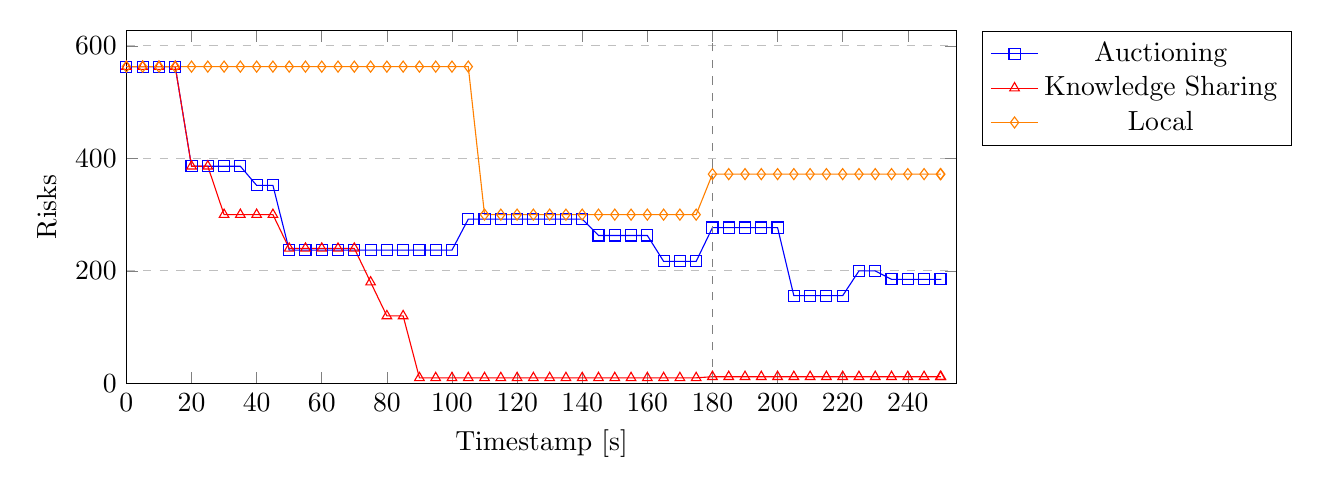
\begin{tikzpicture}
\begin{axis}[
    xlabel={Timestamp [s]},
    ylabel={Risks},
    xmin=0, xmax=255000,
    ymin=0, ymax=627,
    legend pos=outer north east,
    ymajorgrids=true,
    grid style=dashed,
    width=\textwidth,
    height=0.5\textwidth,
    scaled x ticks=base 10:-3,
    xtick scale label code/.code={}
]

	\addplot[color=blue,mark=square] coordinates {
        (0,563)(5000,563)(10000,563)(15000,563)(20000,386)(25000,386)(30000,386)(35000,386)(40000,352)(45000,352)(50000,237)(55000,237)(60000,237)(65000,237)(70000,237)(75000,237)(80000,237)(85000,237)(90000,237)(95000,237)(100000,237)(105000,292)(110000,292)(115000,292)(120000,292)(125000,292)(130000,292)(135000,292)(140000,292)(145000,263)(150000,263)(155000,263)(160000,263)(165000,217)(170000,217)(175000,217)(180000,277)(185000,277)(190000,277)(195000,277)(200000,277)(205000,156)(210000,156)(215000,156)(220000,156)(225000,200)(230000,200)(235000,185)(240000,185)(245000,185)(250000,185)(250288,185)
    };
    \addlegendentry{Auctioning}
	\addplot[color=red,mark=triangle] coordinates {
        (0,563)(5000,563)(10000,563)(15000,563)(20000,386)(25000,386)(30000,300)(35000,300)(40000,300)(45000,300)(50000,240)(55000,240)(60000,240)(65000,240)(70000,240)(75000,180)(80000,120)(85000,120)(90000,10)(95000,10)(100000,10)(105000,10)(110000,10)(115000,10)(120000,10)(125000,10)(130000,10)(135000,10)(140000,10)(145000,10)(150000,10)(155000,10)(160000,10)(165000,10)(170000,10)(175000,10)(180000,12)(185000,12)(190000,12)(195000,12)(200000,12)(205000,12)(210000,12)(215000,12)(220000,12)(225000,12)(230000,12)(235000,12)(240000,12)(245000,12)(250000,12)(250159,12)
    };
    \addlegendentry{Knowledge Sharing}
	\addplot[color=orange,mark=diamond] coordinates {
        (0,563)(5000,563)(10000,563)(15000,563)(20000,563)(25000,563)(30000,563)(35000,563)(40000,563)(45000,563)(50000,563)(55000,563)(60000,563)(65000,563)(70000,563)(75000,563)(80000,563)(85000,563)(90000,563)(95000,563)(100000,563)(105000,563)(110000,300)(115000,300)(120000,300)(125000,300)(130000,300)(135000,300)(140000,300)(145000,300)(150000,300)(155000,300)(160000,300)(165000,300)(170000,300)(175000,300)(180000,372)(185000,372)(190000,372)(195000,372)(200000,372)(205000,372)(210000,372)(215000,372)(220000,372)(225000,372)(230000,372)(235000,372)(240000,372)(245000,372)(250000,372)(250135,372)
    };
    \addlegendentry{Local}

	\addplot[color=gray, dashed,] coordinates {(180000,0) (180000,627)};


\end{axis}
\end{tikzpicture}
    \caption{Graph showing the number of remaining risks in the infrastructure in the risk introduction scenario.}
    \label{fig:risk-remaining-risk-introduction}
\end{figure}

\add{Write}

\begin{figure}[H]
    \centering
        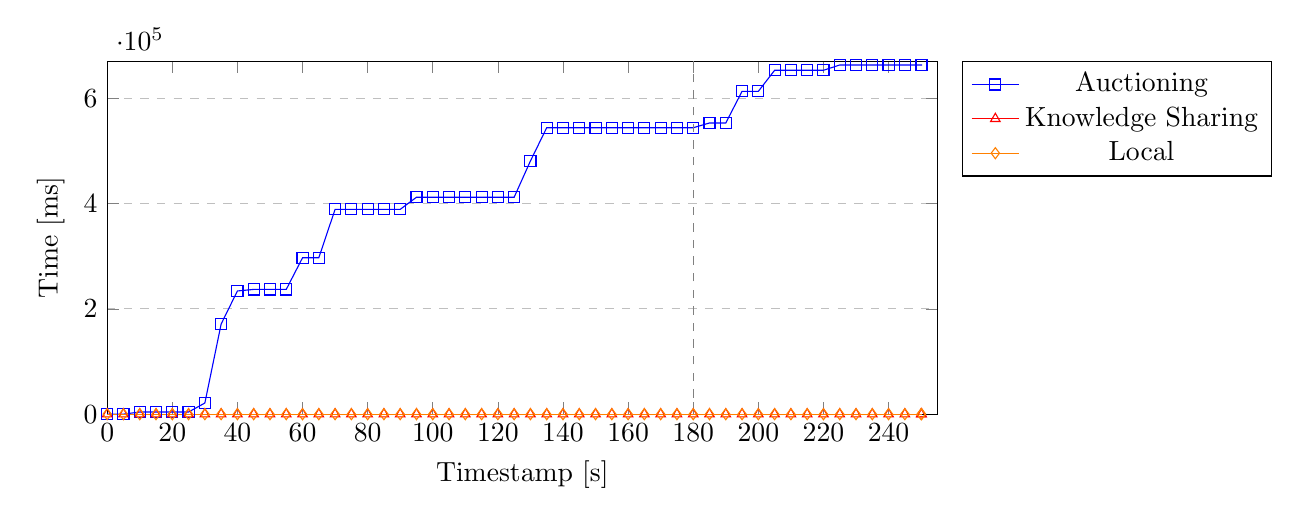
\begin{tikzpicture}
\begin{axis}[
    xlabel={Timestamp [s]},
    ylabel={Time [ms]},
    xmin=0, xmax=255000,
    ymin=0, ymax=670067,
    legend pos=outer north east,
    ymajorgrids=true,
    grid style=dashed,
    width=\textwidth,
    height=0.5\textwidth,
    scaled x ticks=base 10:-3,
    xtick scale label code/.code={}
]

	\addplot[color=blue,mark=square] coordinates {
        (0,0)(5000,64)(10000,4143)(15000,4143)(20000,4143)(25000,4143)(30000,21179)(35000,171183)(40000,233978)(45000,236929)(50000,236929)(55000,236929)(60000,297046)(65000,297049)(70000,388980)(75000,388980)(80000,388980)(85000,388980)(90000,388980)(95000,411980)(100000,411980)(105000,411980)(110000,411980)(115000,411980)(120000,411980)(125000,411980)(130000,480905)(135000,543951)(140000,543951)(145000,543951)(150000,543951)(155000,543958)(160000,543958)(165000,543962)(170000,543962)(175000,543962)(180000,543962)(185000,553054)(190000,553054)(195000,613073)(200000,613073)(205000,653079)(210000,653079)(215000,653087)(220000,653087)(225000,663101)(230000,663101)(235000,663101)(240000,663101)(245000,663101)(250000,663101)(250288,663101)
    };
    \addlegendentry{Auctioning}
	\addplot[color=red,mark=triangle] coordinates {
        (0,0)(5000,0)(10000,0)(15000,0)(20000,0)(25000,0)(30000,0)(35000,0)(40000,0)(45000,0)(50000,0)(55000,0)(60000,0)(65000,0)(70000,0)(75000,0)(80000,0)(85000,0)(90000,0)(95000,0)(100000,0)(105000,0)(110000,0)(115000,0)(120000,0)(125000,0)(130000,0)(135000,0)(140000,0)(145000,0)(150000,0)(155000,0)(160000,0)(165000,0)(170000,0)(175000,0)(180000,0)(185000,0)(190000,0)(195000,0)(200000,0)(205000,0)(210000,0)(215000,0)(220000,0)(225000,0)(230000,0)(235000,0)(240000,0)(245000,0)(250000,0)(250159,0)
    };
    \addlegendentry{Knowledge Sharing}
	\addplot[color=orange,mark=diamond] coordinates {
        (0,0)(5000,0)(10000,0)(15000,0)(20000,0)(25000,0)(30000,0)(35000,0)(40000,0)(45000,0)(50000,0)(55000,0)(60000,0)(65000,0)(70000,0)(75000,0)(80000,0)(85000,0)(90000,0)(95000,0)(100000,0)(105000,0)(110000,0)(115000,0)(120000,0)(125000,0)(130000,0)(135000,0)(140000,0)(145000,0)(150000,0)(155000,0)(160000,0)(165000,0)(170000,0)(175000,0)(180000,0)(185000,0)(190000,0)(195000,0)(200000,0)(205000,0)(210000,0)(215000,0)(220000,0)(225000,0)(230000,0)(235000,0)(240000,0)(245000,0)(250000,0)(250135,0)
    };
    \addlegendentry{Local}

	\addplot[color=gray, dashed,] coordinates {(180000,0) (180000,670067)};


\end{axis}
\end{tikzpicture}
    \caption{Graph showing the sum of time spent auctioning by agents in the risk introduction scenario.}
    \label{fig:auctioning-time-risk-introduction}
\end{figure}

As with figure \ref{fig:auctioning-time-no-change}, we see in figure \ref{fig:adapting-time-risk-introduction} that only the auctioning agent spends time auctioning. The knowledge-sharing agent spends no time auctioning, as it does not have this feature-set. After the $120$ seconds mark we see that the auctioning agent spends more time auctioning, which is a result of the risk being introduced.

\begin{figure}[H]
    \centering
        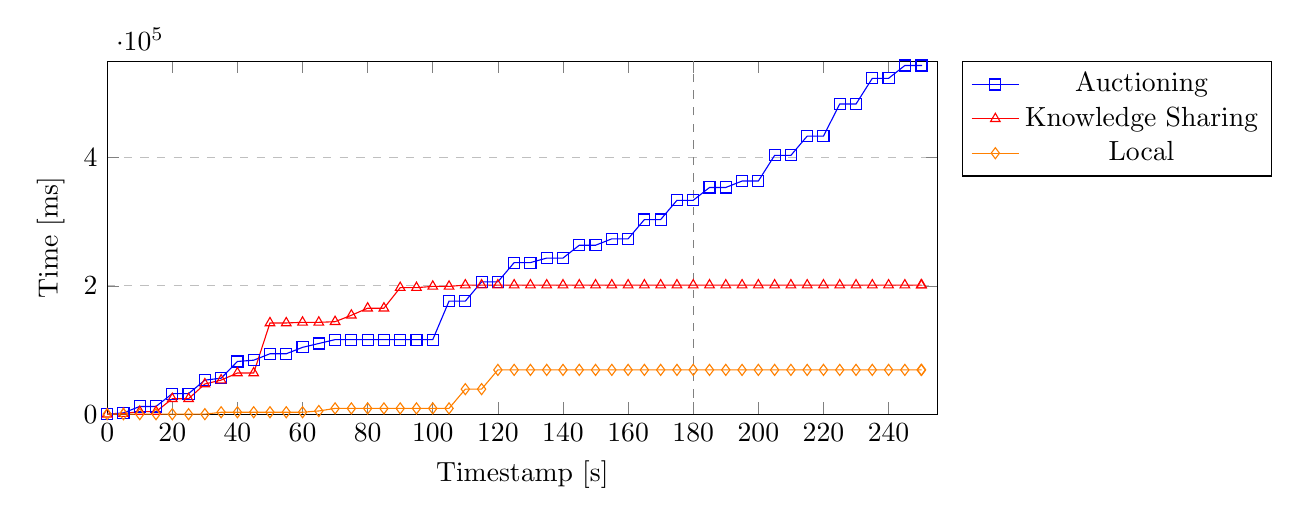
\begin{tikzpicture}
\begin{axis}[
    xlabel={Timestamp [s]},
    ylabel={Time [ms]},
    xmin=0, xmax=255000,
    ymin=0, ymax=550055,
    legend pos=outer north east,
    ymajorgrids=true,
    grid style=dashed,
    width=\textwidth,
    height=0.5\textwidth,
    scaled x ticks=base 10:-3,
    xtick scale label code/.code={}
]

	\addplot[color=blue,mark=square] coordinates {
        (0,0)(5000,2012)(10000,12058)(15000,12058)(20000,32063)(25000,32063)(30000,53081)(35000,56105)(40000,82157)(45000,84176)(50000,94183)(55000,94183)(60000,104190)(65000,110193)(70000,116237)(75000,116237)(80000,116237)(85000,116237)(90000,116237)(95000,116237)(100000,116237)(105000,176271)(110000,176271)(115000,206296)(120000,206296)(125000,236320)(130000,236320)(135000,243360)(140000,243360)(145000,263364)(150000,263364)(155000,273368)(160000,273368)(165000,303394)(170000,303394)(175000,333415)(180000,333415)(185000,353427)(190000,353427)(195000,363436)(200000,363436)(205000,403461)(210000,403461)(215000,433478)(220000,433478)(225000,483523)(230000,483523)(235000,523553)(240000,523553)(245000,543563)(250000,543563)(250288,543563)
    };
    \addlegendentry{Auctioning}
	\addplot[color=red,mark=triangle] coordinates {
        (0,0)(5000,1005)(10000,4021)(15000,4021)(20000,24028)(25000,24028)(30000,47052)(35000,53154)(40000,64163)(45000,64163)(50000,142192)(55000,142192)(60000,143196)(65000,143196)(70000,144197)(75000,154200)(80000,165206)(85000,165206)(90000,197224)(95000,197224)(100000,199232)(105000,199232)(110000,201240)(115000,201240)(120000,201240)(125000,201240)(130000,201240)(135000,201240)(140000,201240)(145000,201240)(150000,201240)(155000,201240)(160000,201240)(165000,201240)(170000,201240)(175000,201240)(180000,201240)(185000,201240)(190000,201240)(195000,201240)(200000,201240)(205000,201240)(210000,201240)(215000,201240)(220000,201240)(225000,201240)(230000,201240)(235000,201240)(240000,201240)(245000,201240)(250000,201240)(250159,201240)
    };
    \addlegendentry{Knowledge Sharing}
	\addplot[color=orange,mark=diamond] coordinates {
        (0,0)(5000,0)(10000,0)(15000,0)(20000,0)(25000,0)(30000,0)(35000,3017)(40000,3017)(45000,3017)(50000,3017)(55000,3017)(60000,3017)(65000,5025)(70000,9035)(75000,9035)(80000,9035)(85000,9035)(90000,9035)(95000,9035)(100000,9035)(105000,9035)(110000,39044)(115000,39044)(120000,69058)(125000,69058)(130000,69058)(135000,69058)(140000,69058)(145000,69058)(150000,69058)(155000,69058)(160000,69058)(165000,69058)(170000,69058)(175000,69058)(180000,69058)(185000,69058)(190000,69058)(195000,69058)(200000,69058)(205000,69058)(210000,69058)(215000,69058)(220000,69058)(225000,69058)(230000,69058)(235000,69058)(240000,69058)(245000,69058)(250000,69058)(250135,69058)
    };
    \addlegendentry{Local}

	\addplot[color=gray, dashed,] coordinates {(180000,0) (180000,550055)};


\end{axis}
\end{tikzpicture}
    \caption{Graph showing the sum of time spent adapting by agents in the risk introduction scenario.}
    \label{fig:adapting-time-risk-introduction}
\end{figure}

Figure \ref{fig:adapting-time-risk-introduction} shows that the knowledge-sharing agent is still spending more time adapting compared to the auctioning agent. Compared to figure \ref{fig:adapting-time-no-change} we see that the agents are all spending roughly the same amount of time adapting, until the $120$ second mark. After this time a bump is observable in the graph.

\subsection{Scenario 3: Growing Infrastructure}
\textit{This scenario introduces a new infrastructure node every $30$ seconds. The purpose of this scenario is to see how the system behaves when the infrastructure is growing.}

\begin{figure}[H]
    \centering
    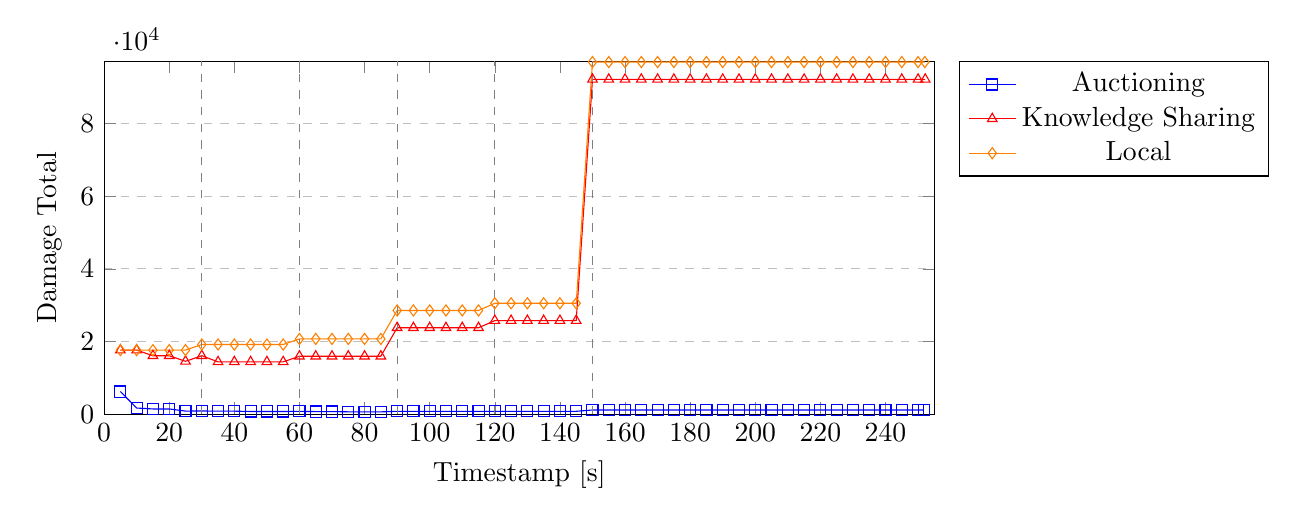
\begin{tikzpicture}
\begin{axis}[
    xlabel={Timestamp [s]},
    ylabel={Damage Total},
    xmin=0, xmax=255000,
    ymin=0, ymax=97097,
    legend pos=outer north east,
    ymajorgrids=true,
    grid style=dashed,
    width=\textwidth,
    height=0.5\textwidth,
    scaled x ticks=base 10:-3,
    xtick scale label code/.code={}
]

	\addplot[color=blue,mark=square] coordinates {
        (5000,6236.51)(10000,1693.70)(15000,1442.78)(20000,1442.78)(25000,857.00)(30000,882.24)(35000,830.70)(40000,830.70)(45000,747.92)(50000,747.92)(55000,747.92)(60000,775.51)(65000,722.54)(70000,722.54)(75000,654.66)(80000,645.84)(85000,645.84)(90000,786.16)(95000,786.16)(100000,786.16)(105000,786.16)(110000,786.16)(115000,786.16)(120000,794.99)(125000,794.99)(130000,794.99)(135000,794.99)(140000,794.99)(145000,794.99)(150000,1153.85)(155000,1153.85)(160000,1153.85)(165000,1153.85)(170000,1153.85)(175000,1153.85)(180000,1153.85)(185000,1153.85)(190000,1153.85)(195000,1153.85)(200000,1153.85)(205000,1153.85)(210000,1153.85)(215000,1153.85)(220000,1153.85)(225000,1153.85)(230000,1153.85)(235000,1153.85)(240000,1153.85)(245000,1153.85)(250000,1153.85)(251808,1153.85)
    };
    \addlegendentry{Auctioning}
	\addplot[color=red,mark=triangle] coordinates {
        (5000,17629.95)(10000,17629.95)(15000,16089.24)(20000,16089.24)(25000,14548.54)(30000,16089.24)(35000,14404.74)(40000,14404.74)(45000,14404.74)(50000,14404.74)(55000,14404.74)(60000,15945.45)(65000,15945.45)(70000,15945.45)(75000,15945.45)(80000,15945.45)(85000,15945.45)(90000,23781.19)(95000,23781.19)(100000,23781.19)(105000,23781.19)(110000,23781.19)(115000,23781.19)(120000,25753.29)(125000,25753.29)(130000,25753.29)(135000,25753.29)(140000,25753.29)(145000,25753.29)(150000,92136.15)(155000,92136.15)(160000,92136.15)(165000,92136.15)(170000,92136.15)(175000,92136.15)(180000,92136.15)(185000,92136.15)(190000,92136.15)(195000,92136.15)(200000,92136.15)(205000,92136.15)(210000,92136.15)(215000,92136.15)(220000,92136.15)(225000,92136.15)(230000,92136.15)(235000,92136.15)(240000,92136.15)(245000,92136.15)(250000,92136.15)(252200,92136.15)
    };
    \addlegendentry{Knowledge Sharing}
	\addplot[color=orange,mark=diamond] coordinates {
        (5000,17629.95)(10000,17629.95)(15000,17629.95)(20000,17629.95)(25000,17629.95)(30000,19170.65)(35000,19170.65)(40000,19170.65)(45000,19170.65)(50000,19170.65)(55000,19170.65)(60000,20711.36)(65000,20711.36)(70000,20711.36)(75000,20711.36)(80000,20711.36)(85000,20711.36)(90000,28547.10)(95000,28547.10)(100000,28547.10)(105000,28547.10)(110000,28547.10)(115000,28547.10)(120000,30519.20)(125000,30519.20)(130000,30519.20)(135000,30519.20)(140000,30519.20)(145000,30519.20)(150000,96902.06)(155000,96902.06)(160000,96902.06)(165000,96902.06)(170000,96902.06)(175000,96902.06)(180000,96902.06)(185000,96902.06)(190000,96902.06)(195000,96902.06)(200000,96902.06)(205000,96902.06)(210000,96902.06)(215000,96902.06)(220000,96902.06)(225000,96902.06)(230000,96902.06)(235000,96902.06)(240000,96902.06)(245000,96902.06)(250000,96902.06)(252076,96902.06)
    };
    \addlegendentry{Local}

	\addplot[color=gray, dashed,] coordinates {(30000,0) (30000,97097)};
	\addplot[color=gray, dashed,] coordinates {(60000,0) (60000,97097)};
	\addplot[color=gray, dashed,] coordinates {(90000,0) (90000,97097)};
	\addplot[color=gray, dashed,] coordinates {(120000,0) (120000,97097)};
	\addplot[color=gray, dashed,] coordinates {(150000,0) (150000,97097)};


\end{axis}
\end{tikzpicture}
    \caption{This graph shows the overall damage of the system in the growing scenario. The damage is shown for each of the three strategies. The vertical lines indicate the time at which a node is introduced.}
    \label{fig:overall-damage-growing}
\end{figure}

From Figure \ref{fig:overall-damage-growing} we see that the auctioning and knowledge-sharing agents are able to keep the damage at a stable level, even though the infrastructure is growing. Only at the end do we see that the agents cannot cope with the increasing damage and does the damage increase. The auctioning agent is keeping the overall damage at the lowest point. This is a good result, as the infrastructure is growing, and the agents are able to keep the damage at a low level. 
As mentioned before, the damage is calculated at a $5000$ms interval. This means that the damage could be higher than the graph shows, as adaptations could be applied within the timeframe. This is the case for the auctioning agent and knowledge-sharing agent, which is observed in the log-files. However, the local-agent does not apply any adaptations during this time, this is visible in the diverging lines at the end of the graph.
 
\begin{figure}[H]
    \centering
    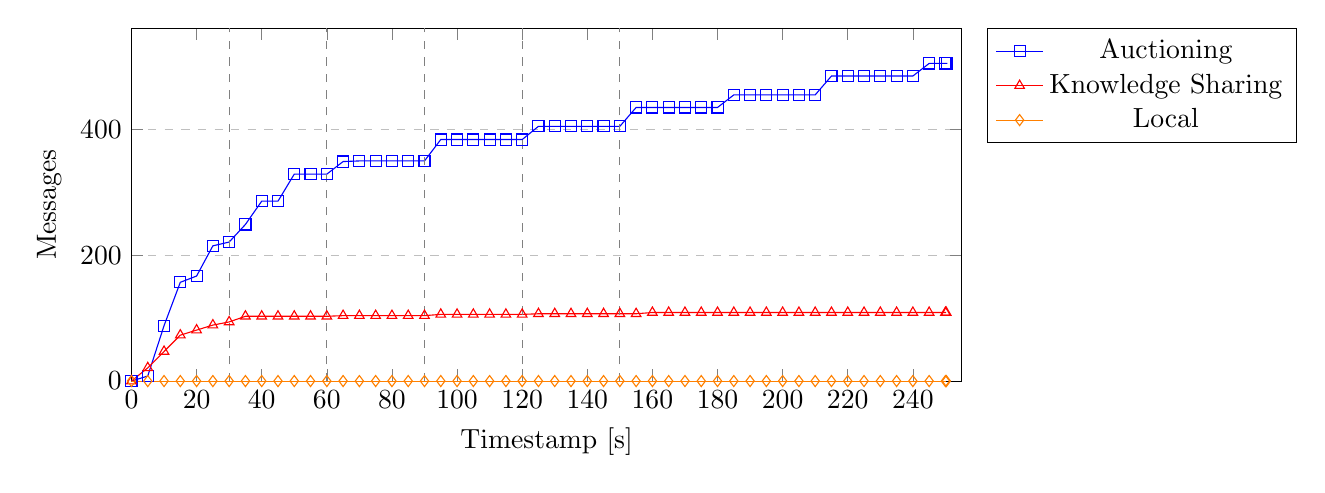
\begin{tikzpicture}
\begin{axis}[
    xlabel={Timestamp [s]},
    ylabel={Messages},
    xmin=0, xmax=255000,
    ymin=0, ymax=561,
    legend pos=outer north east,
    ymajorgrids=true,
    grid style=dashed,
    width=\textwidth,
    height=0.5\textwidth,
    scaled x ticks=base 10:-3,
    xtick scale label code/.code={}
]

	\addplot[color=blue,mark=square] coordinates {
        (0,0)(5000,8)(10000,88)(15000,157)(20000,167)(25000,215)(30000,221)(35000,249)(40000,286)(45000,286)(50000,329)(55000,329)(60000,329)(65000,349)(70000,350)(75000,350)(80000,350)(85000,350)(90000,350)(95000,384)(100000,384)(105000,384)(110000,384)(115000,384)(120000,384)(125000,405)(130000,405)(135000,405)(140000,405)(145000,405)(150000,405)(155000,435)(160000,435)(165000,435)(170000,435)(175000,435)(180000,435)(185000,455)(190000,455)(195000,455)(200000,455)(205000,455)(210000,455)(215000,485)(220000,485)(225000,485)(230000,485)(235000,485)(240000,485)(245000,505)(250000,505)(250569,505)
    };
    \addlegendentry{Auctioning}
	\addplot[color=red,mark=triangle] coordinates {
        (0,0)(5000,21)(10000,47)(15000,73)(20000,81)(25000,89)(30000,94)(35000,103)(40000,103)(45000,103)(50000,103)(55000,103)(60000,103)(65000,104)(70000,104)(75000,104)(80000,104)(85000,104)(90000,104)(95000,106)(100000,106)(105000,106)(110000,106)(115000,106)(120000,106)(125000,107)(130000,107)(135000,107)(140000,107)(145000,107)(150000,107)(155000,107)(160000,109)(165000,109)(170000,109)(175000,109)(180000,109)(185000,109)(190000,109)(195000,109)(200000,109)(205000,109)(210000,109)(215000,109)(220000,109)(225000,109)(230000,109)(235000,109)(240000,109)(245000,109)(250000,109)(250242,109)
    };
    \addlegendentry{Knowledge Sharing}
	\addplot[color=orange,mark=diamond] coordinates {
        (0,0)(5000,0)(10000,0)(15000,0)(20000,0)(25000,0)(30000,0)(35000,0)(40000,0)(45000,0)(50000,0)(55000,0)(60000,0)(65000,0)(70000,0)(75000,0)(80000,0)(85000,0)(90000,0)(95000,0)(100000,0)(105000,0)(110000,0)(115000,0)(120000,0)(125000,0)(130000,0)(135000,0)(140000,0)(145000,0)(150000,0)(155000,0)(160000,0)(165000,0)(170000,0)(175000,0)(180000,0)(185000,0)(190000,0)(195000,0)(200000,0)(205000,0)(210000,0)(215000,0)(220000,0)(225000,0)(230000,0)(235000,0)(240000,0)(245000,0)(250000,0)(250282,0)
    };
    \addlegendentry{Local}

	\addplot[color=gray, dashed,] coordinates {(30000,0) (30000,561)};
	\addplot[color=gray, dashed,] coordinates {(60000,0) (60000,561)};
	\addplot[color=gray, dashed,] coordinates {(90000,0) (90000,561)};
	\addplot[color=gray, dashed,] coordinates {(120000,0) (120000,561)};
	\addplot[color=gray, dashed,] coordinates {(150000,0) (150000,561)};


\end{axis}
\end{tikzpicture}
    \caption{Graph showing the total amount of messages sent between agents in the growing infrastructure scenario.}
    \label{fig:messages-growing}
\end{figure}

Figure \ref{fig:messages-growing} shows that the auctioning agent sends the most messages, followed by the knowledge-sharing agent. The local-agent sends no messages. We see that both the auctioning and knowledge-sharing agents send a few messages around every time a new node is introduced. This is to be expected as the agents detect a change in their properties, and start sharing this information with other agents.

\begin{figure}[H]
    \centering
    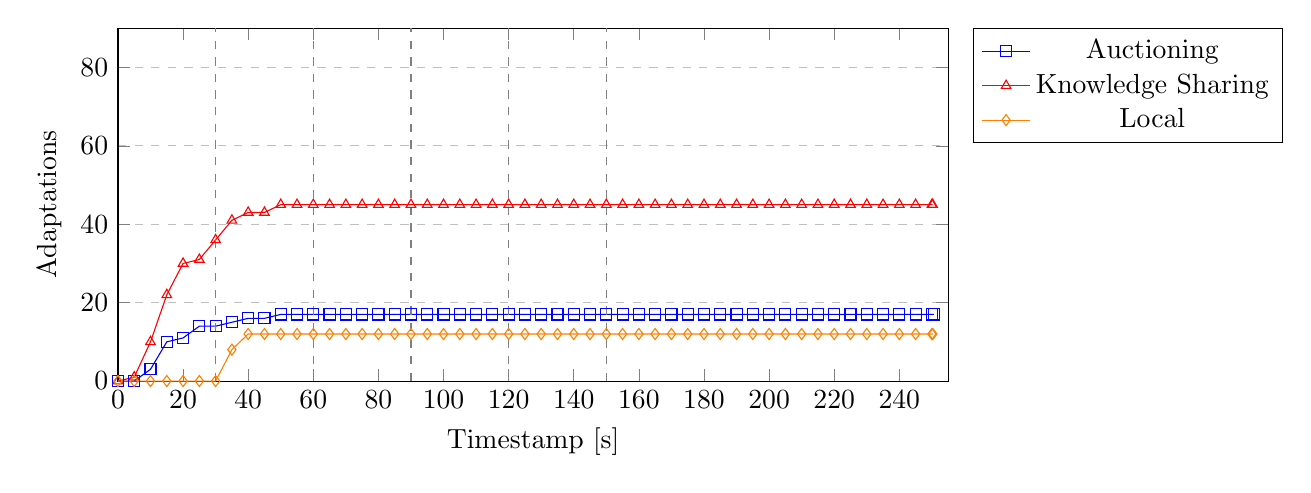
\begin{tikzpicture}
\begin{axis}[
    xlabel={Timestamp [s]},
    ylabel={Adaptations},
    xmin=0, xmax=255000,
    ymin=0, ymax=90,
    legend pos=outer north east,
    ymajorgrids=true,
    grid style=dashed,
    width=\textwidth,
    height=0.5\textwidth,
    scaled x ticks=base 10:-3,
    xtick scale label code/.code={}
]

	\addplot[color=blue,mark=square] coordinates {
        (0,0)(5000,0)(10000,3)(15000,10)(20000,11)(25000,14)(30000,14)(35000,15)(40000,16)(45000,16)(50000,17)(55000,17)(60000,17)(65000,17)(70000,17)(75000,17)(80000,17)(85000,17)(90000,17)(95000,17)(100000,17)(105000,17)(110000,17)(115000,17)(120000,17)(125000,17)(130000,17)(135000,17)(140000,17)(145000,17)(150000,17)(155000,17)(160000,17)(165000,17)(170000,17)(175000,17)(180000,17)(185000,17)(190000,17)(195000,17)(200000,17)(205000,17)(210000,17)(215000,17)(220000,17)(225000,17)(230000,17)(235000,17)(240000,17)(245000,17)(250000,17)(250569,17)
    };
    \addlegendentry{Auctioning}
	\addplot[color=red,mark=triangle] coordinates {
        (0,0)(5000,1)(10000,10)(15000,22)(20000,30)(25000,31)(30000,36)(35000,41)(40000,43)(45000,43)(50000,45)(55000,45)(60000,45)(65000,45)(70000,45)(75000,45)(80000,45)(85000,45)(90000,45)(95000,45)(100000,45)(105000,45)(110000,45)(115000,45)(120000,45)(125000,45)(130000,45)(135000,45)(140000,45)(145000,45)(150000,45)(155000,45)(160000,45)(165000,45)(170000,45)(175000,45)(180000,45)(185000,45)(190000,45)(195000,45)(200000,45)(205000,45)(210000,45)(215000,45)(220000,45)(225000,45)(230000,45)(235000,45)(240000,45)(245000,45)(250000,45)(250242,45)
    };
    \addlegendentry{Knowledge Sharing}
	\addplot[color=orange,mark=diamond] coordinates {
        (0,0)(5000,0)(10000,0)(15000,0)(20000,0)(25000,0)(30000,0)(35000,8)(40000,12)(45000,12)(50000,12)(55000,12)(60000,12)(65000,12)(70000,12)(75000,12)(80000,12)(85000,12)(90000,12)(95000,12)(100000,12)(105000,12)(110000,12)(115000,12)(120000,12)(125000,12)(130000,12)(135000,12)(140000,12)(145000,12)(150000,12)(155000,12)(160000,12)(165000,12)(170000,12)(175000,12)(180000,12)(185000,12)(190000,12)(195000,12)(200000,12)(205000,12)(210000,12)(215000,12)(220000,12)(225000,12)(230000,12)(235000,12)(240000,12)(245000,12)(250000,12)(250282,12)
    };
    \addlegendentry{Local}

	\addplot[color=gray, dashed,] coordinates {(30000,0) (30000,90)};
	\addplot[color=gray, dashed,] coordinates {(60000,0) (60000,90)};
	\addplot[color=gray, dashed,] coordinates {(90000,0) (90000,90)};
	\addplot[color=gray, dashed,] coordinates {(120000,0) (120000,90)};
	\addplot[color=gray, dashed,] coordinates {(150000,0) (150000,90)};


\end{axis}
\end{tikzpicture}
    \caption{Graph showing the total amount of adaptations applied by agents in the growing scenario.}
    \label{fig:proposals-growing}
\end{figure}

As for the adaptations in this experiment, we also see a gradual increase in proposals over time. The local agent is unable to cope with the changes to the infrastructure, and is unable to apply any adaptations. We see that the auctioning agent is slowly applying adaptations, where the knowledge-sharing agent applies them like in quick succession. This is to be expected as the auctioning agent has to negotiate the adaptations, which takes time.

\begin{figure}[H]
    \centering
        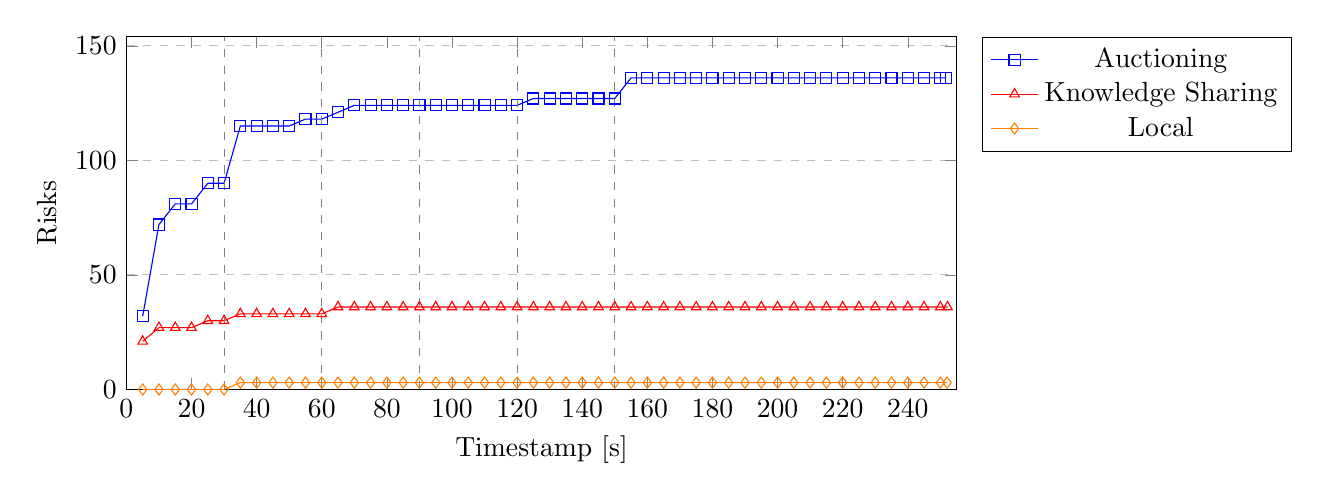
\begin{tikzpicture}
\begin{axis}[
    xlabel={Timestamp [s]},
    ylabel={Risks},
    xmin=0, xmax=255000,
    ymin=0, ymax=154,
    legend pos=outer north east,
    ymajorgrids=true,
    grid style=dashed,
    width=\textwidth,
    height=0.5\textwidth,
    scaled x ticks=base 10:-3,
    xtick scale label code/.code={}
]

	\addplot[color=blue,mark=square] coordinates {
        (5000,32)(10000,72)(15000,81)(20000,81)(25000,90)(30000,90)(35000,115)(40000,115)(45000,115)(50000,115)(55000,118)(60000,118)(65000,121)(70000,124)(75000,124)(80000,124)(85000,124)(90000,124)(95000,124)(100000,124)(105000,124)(110000,124)(115000,124)(120000,124)(125000,127)(130000,127)(135000,127)(140000,127)(145000,127)(150000,127)(155000,136)(160000,136)(165000,136)(170000,136)(175000,136)(180000,136)(185000,136)(190000,136)(195000,136)(200000,136)(205000,136)(210000,136)(215000,136)(220000,136)(225000,136)(230000,136)(235000,136)(240000,136)(245000,136)(250000,136)(251808,136)
    };
    \addlegendentry{Auctioning}
	\addplot[color=red,mark=triangle] coordinates {
        (5000,21)(10000,27)(15000,27)(20000,27)(25000,30)(30000,30)(35000,33)(40000,33)(45000,33)(50000,33)(55000,33)(60000,33)(65000,36)(70000,36)(75000,36)(80000,36)(85000,36)(90000,36)(95000,36)(100000,36)(105000,36)(110000,36)(115000,36)(120000,36)(125000,36)(130000,36)(135000,36)(140000,36)(145000,36)(150000,36)(155000,36)(160000,36)(165000,36)(170000,36)(175000,36)(180000,36)(185000,36)(190000,36)(195000,36)(200000,36)(205000,36)(210000,36)(215000,36)(220000,36)(225000,36)(230000,36)(235000,36)(240000,36)(245000,36)(250000,36)(252200,36)
    };
    \addlegendentry{Knowledge Sharing}
	\addplot[color=orange,mark=diamond] coordinates {
        (5000,0)(10000,0)(15000,0)(20000,0)(25000,0)(30000,0)(35000,3)(40000,3)(45000,3)(50000,3)(55000,3)(60000,3)(65000,3)(70000,3)(75000,3)(80000,3)(85000,3)(90000,3)(95000,3)(100000,3)(105000,3)(110000,3)(115000,3)(120000,3)(125000,3)(130000,3)(135000,3)(140000,3)(145000,3)(150000,3)(155000,3)(160000,3)(165000,3)(170000,3)(175000,3)(180000,3)(185000,3)(190000,3)(195000,3)(200000,3)(205000,3)(210000,3)(215000,3)(220000,3)(225000,3)(230000,3)(235000,3)(240000,3)(245000,3)(250000,3)(252076,3)
    };
    \addlegendentry{Local}

	\addplot[color=gray, dashed,] coordinates {(30000,0) (30000,154)};
	\addplot[color=gray, dashed,] coordinates {(60000,0) (60000,154)};
	\addplot[color=gray, dashed,] coordinates {(90000,0) (90000,154)};
	\addplot[color=gray, dashed,] coordinates {(120000,0) (120000,154)};
	\addplot[color=gray, dashed,] coordinates {(150000,0) (150000,154)};


\end{axis}
\end{tikzpicture}
    \caption{Graph showing the number of unique risks detected by agents in the growing scenario.}
    \label{fig:risk-count-growing}
\end{figure}

Figure \ref{fig:risk-count-growing} show that the knowledge-sharing agent finds the most unique risks, followed by the auctioning agent. The auctioning agent finds only $50\%$ of the risks detected by the knowledge-sharing agent. The local-agent finds the least amount of risks, at only $10\%$ of the risks found by the knowledge-sharing agent. As mentioned in Section \ref{ssec:scenario-2-results}, this is likely due to the fact that in the knowledge-sharing setup agents apply multiple adaptations in parallel. 

\begin{figure}[H]
    \centering
        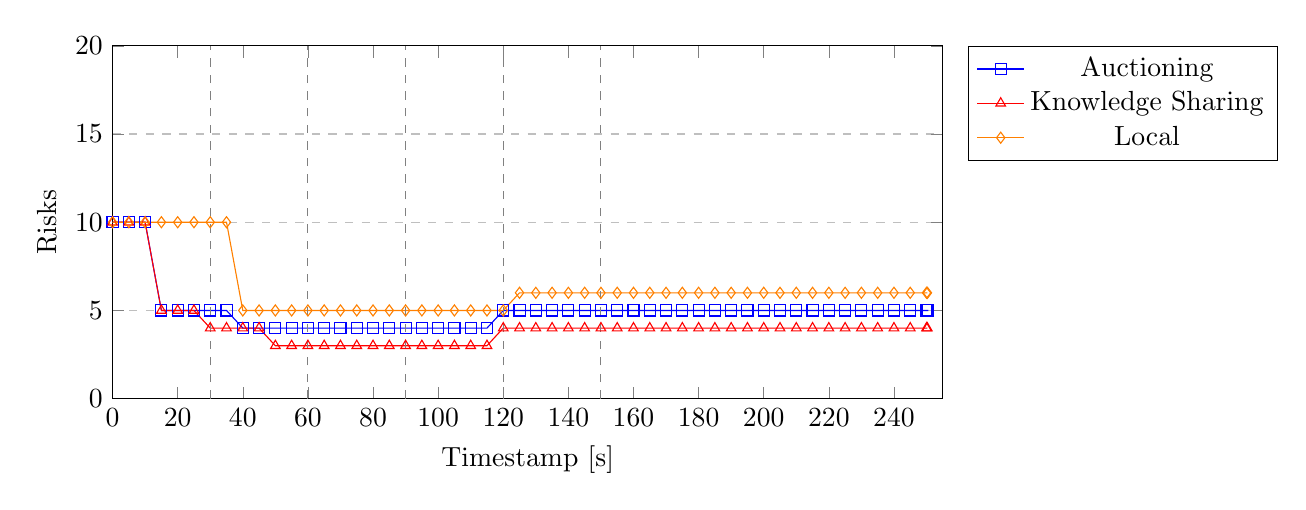
\begin{tikzpicture}
\begin{axis}[
    xlabel={Timestamp [s]},
    ylabel={Risks},
    xmin=0, xmax=255000,
    ymin=0, ymax=20,
    legend pos=outer north east,
    ymajorgrids=true,
    grid style=dashed,
    width=\textwidth,
    height=0.5\textwidth,
    scaled x ticks=base 10:-3,
    xtick scale label code/.code={}
]

	\addplot[color=blue,mark=square] coordinates {
        (0,10)(5000,10)(10000,10)(15000,5)(20000,5)(25000,5)(30000,5)(35000,5)(40000,4)(45000,4)(50000,4)(55000,4)(60000,4)(65000,4)(70000,4)(75000,4)(80000,4)(85000,4)(90000,4)(95000,4)(100000,4)(105000,4)(110000,4)(115000,4)(120000,5)(125000,5)(130000,5)(135000,5)(140000,5)(145000,5)(150000,5)(155000,5)(160000,5)(165000,5)(170000,5)(175000,5)(180000,5)(185000,5)(190000,5)(195000,5)(200000,5)(205000,5)(210000,5)(215000,5)(220000,5)(225000,5)(230000,5)(235000,5)(240000,5)(245000,5)(250000,5)(250569,5)
    };
    \addlegendentry{Auctioning}
	\addplot[color=red,mark=triangle] coordinates {
        (0,10)(5000,10)(10000,10)(15000,5)(20000,5)(25000,5)(30000,4)(35000,4)(40000,4)(45000,4)(50000,3)(55000,3)(60000,3)(65000,3)(70000,3)(75000,3)(80000,3)(85000,3)(90000,3)(95000,3)(100000,3)(105000,3)(110000,3)(115000,3)(120000,4)(125000,4)(130000,4)(135000,4)(140000,4)(145000,4)(150000,4)(155000,4)(160000,4)(165000,4)(170000,4)(175000,4)(180000,4)(185000,4)(190000,4)(195000,4)(200000,4)(205000,4)(210000,4)(215000,4)(220000,4)(225000,4)(230000,4)(235000,4)(240000,4)(245000,4)(250000,4)(250242,4)
    };
    \addlegendentry{Knowledge Sharing}
	\addplot[color=orange,mark=diamond] coordinates {
        (0,10)(5000,10)(10000,10)(15000,10)(20000,10)(25000,10)(30000,10)(35000,10)(40000,5)(45000,5)(50000,5)(55000,5)(60000,5)(65000,5)(70000,5)(75000,5)(80000,5)(85000,5)(90000,5)(95000,5)(100000,5)(105000,5)(110000,5)(115000,5)(120000,5)(125000,6)(130000,6)(135000,6)(140000,6)(145000,6)(150000,6)(155000,6)(160000,6)(165000,6)(170000,6)(175000,6)(180000,6)(185000,6)(190000,6)(195000,6)(200000,6)(205000,6)(210000,6)(215000,6)(220000,6)(225000,6)(230000,6)(235000,6)(240000,6)(245000,6)(250000,6)(250282,6)
    };
    \addlegendentry{Local}

	\addplot[color=gray, dashed,] coordinates {(30000,0) (30000,20)};
	\addplot[color=gray, dashed,] coordinates {(60000,0) (60000,20)};
	\addplot[color=gray, dashed,] coordinates {(90000,0) (90000,20)};
	\addplot[color=gray, dashed,] coordinates {(120000,0) (120000,20)};
	\addplot[color=gray, dashed,] coordinates {(150000,0) (150000,20)};


\end{axis}
\end{tikzpicture}
    \caption{Graph showing the number of remaining risks in the infrastructure in the growing scenario.}
    \label{fig:risk-remaining-growing}
\end{figure}

\add{write}

\begin{figure}[H]
    \centering
        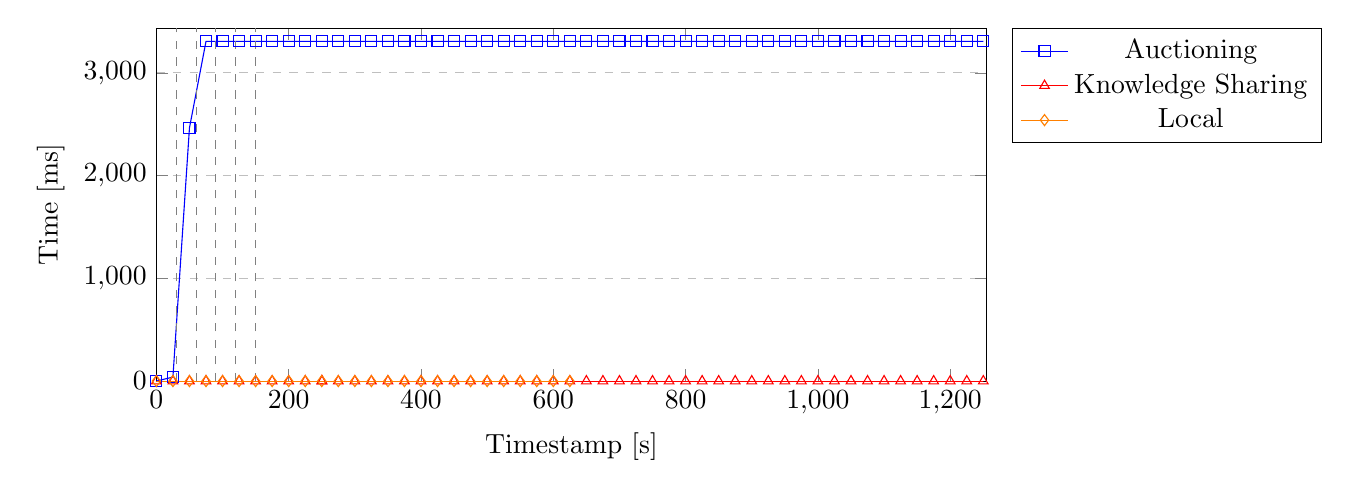
\begin{tikzpicture}
\begin{axis}[
    xlabel={Timestamp [s]},
    ylabel={Time [ms]},
    xmin=0, xmax=1255000,
    ymin=0, ymax=3434,
    legend pos=outer north east,
    ymajorgrids=true,
    grid style=dashed,
    width=\textwidth,
    height=0.5\textwidth,
    scaled x ticks=base 10:-3,
    xtick scale label code/.code={}
]

	\addplot[color=blue,mark=square] coordinates {
        (0,0)(25000,39)(50000,2464)(75000,3306)(100000,3306)(125000,3306)(150000,3306)(175000,3306)(200000,3306)(225000,3306)(250000,3306)(275000,3306)(300000,3306)(325000,3306)(350000,3306)(375000,3306)(400000,3306)(425000,3306)(450000,3306)(475000,3306)(500000,3306)(525000,3306)(550000,3306)(575000,3306)(600000,3306)(625000,3306)(650000,3306)(675000,3306)(700000,3306)(725000,3306)(750000,3306)(775000,3306)(800000,3306)(825000,3306)(850000,3306)(875000,3306)(900000,3306)(925000,3306)(950000,3306)(975000,3306)(1000000,3306)(1025000,3306)(1050000,3306)(1075000,3306)(1100000,3306)(1125000,3306)(1150000,3306)(1175000,3306)(1200000,3306)(1225000,3306)(1250000,3306)(250447,3306)
    };
    \addlegendentry{Auctioning}
	\addplot[color=red,mark=triangle] coordinates {
        (0,0)(25000,0)(50000,0)(75000,0)(100000,0)(125000,0)(150000,0)(175000,0)(200000,0)(225000,0)(250000,0)(275000,0)(300000,0)(325000,0)(350000,0)(375000,0)(400000,0)(425000,0)(450000,0)(475000,0)(500000,0)(525000,0)(550000,0)(575000,0)(600000,0)(625000,0)(650000,0)(675000,0)(700000,0)(725000,0)(750000,0)(775000,0)(800000,0)(825000,0)(850000,0)(875000,0)(900000,0)(925000,0)(950000,0)(975000,0)(1000000,0)(1025000,0)(1050000,0)(1075000,0)(1100000,0)(1125000,0)(1150000,0)(1175000,0)(1200000,0)(1225000,0)(1250000,0)(250418,0)
    };
    \addlegendentry{Knowledge Sharing}
	\addplot[color=orange,mark=diamond] coordinates {
        (0,0)(25000,0)(50000,0)(75000,0)(100000,0)(125000,0)(150000,0)(175000,0)(200000,0)(225000,0)(250000,0)(275000,0)(300000,0)(325000,0)(350000,0)(375000,0)(400000,0)(425000,0)(450000,0)(475000,0)(500000,0)(525000,0)(550000,0)(575000,0)(600000,0)(625000,0)
    };
    \addlegendentry{Local}

	\addplot[color=gray, dashed,] coordinates {(30000,0) (30000,3434)};
	\addplot[color=gray, dashed,] coordinates {(60000,0) (60000,3434)};
	\addplot[color=gray, dashed,] coordinates {(90000,0) (90000,3434)};
	\addplot[color=gray, dashed,] coordinates {(120000,0) (120000,3434)};
	\addplot[color=gray, dashed,] coordinates {(150000,0) (150000,3434)};


\end{axis}
\end{tikzpicture}
    \caption{Graph showing the sum of time spent auctioning by agents in the growing scenario.}
    \label{fig:auctioning-time-growing}
\end{figure}

Figure \ref{fig:auctioning-time-growing} shows an ever growing amount of time spent auctioning. This is in line with the expectations as the agents finds a risk, and then starts an auction. These auctions in the end lead to no proposals/adaptations being applied, as the agents are unable to find a better adaptation. This is visible in the graph as the time spent auctioning increases, but the amount of adaptations from Figure \ref{fig:proposals-growing} stays the same.

\begin{figure}[H]
    \centering
        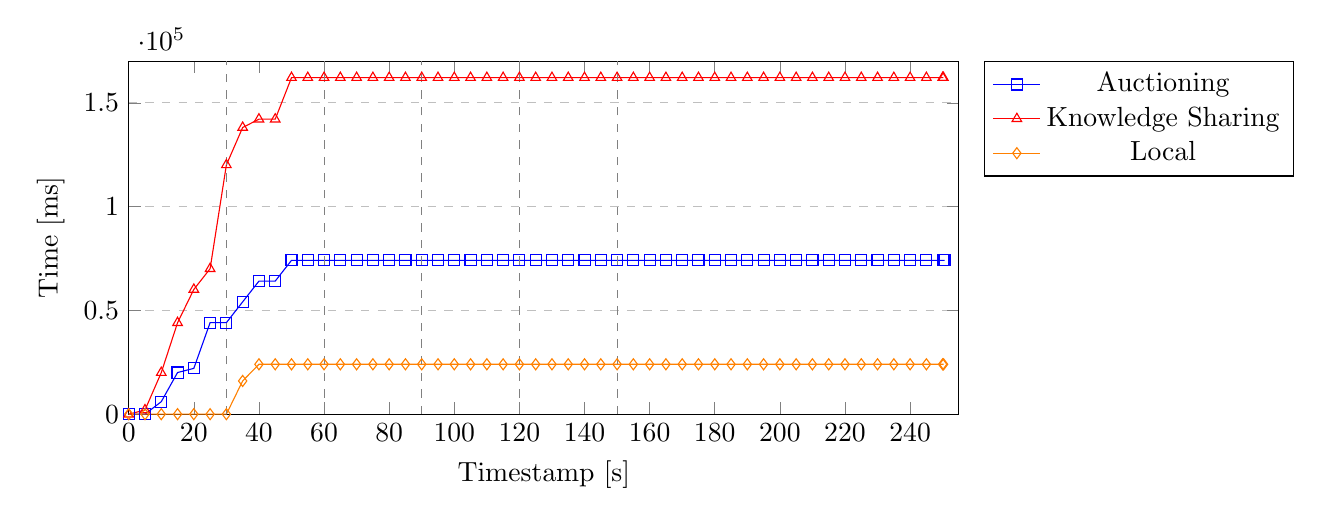
\begin{tikzpicture}
\begin{axis}[
    xlabel={Timestamp [s]},
    ylabel={Time [ms]},
    xmin=0, xmax=255000,
    ymin=0, ymax=170017,
    legend pos=outer north east,
    ymajorgrids=true,
    grid style=dashed,
    width=\textwidth,
    height=0.5\textwidth,
    scaled x ticks=base 10:-3,
    xtick scale label code/.code={}
]

	\addplot[color=blue,mark=square] coordinates {
        (0,0)(5000,0)(10000,6018)(15000,20071)(20000,22078)(25000,44102)(30000,44102)(35000,54111)(40000,64119)(45000,64119)(50000,74128)(55000,74128)(60000,74128)(65000,74128)(70000,74128)(75000,74128)(80000,74128)(85000,74128)(90000,74128)(95000,74128)(100000,74128)(105000,74128)(110000,74128)(115000,74128)(120000,74128)(125000,74128)(130000,74128)(135000,74128)(140000,74128)(145000,74128)(150000,74128)(155000,74128)(160000,74128)(165000,74128)(170000,74128)(175000,74128)(180000,74128)(185000,74128)(190000,74128)(195000,74128)(200000,74128)(205000,74128)(210000,74128)(215000,74128)(220000,74128)(225000,74128)(230000,74128)(235000,74128)(240000,74128)(245000,74128)(250000,74128)(250569,74128)
    };
    \addlegendentry{Auctioning}
	\addplot[color=red,mark=triangle] coordinates {
        (0,0)(5000,2004)(10000,20023)(15000,44059)(20000,60095)(25000,70097)(30000,120113)(35000,138132)(40000,142140)(45000,142140)(50000,162147)(55000,162147)(60000,162147)(65000,162147)(70000,162147)(75000,162147)(80000,162147)(85000,162147)(90000,162147)(95000,162147)(100000,162147)(105000,162147)(110000,162147)(115000,162147)(120000,162147)(125000,162147)(130000,162147)(135000,162147)(140000,162147)(145000,162147)(150000,162147)(155000,162147)(160000,162147)(165000,162147)(170000,162147)(175000,162147)(180000,162147)(185000,162147)(190000,162147)(195000,162147)(200000,162147)(205000,162147)(210000,162147)(215000,162147)(220000,162147)(225000,162147)(230000,162147)(235000,162147)(240000,162147)(245000,162147)(250000,162147)(250242,162147)
    };
    \addlegendentry{Knowledge Sharing}
	\addplot[color=orange,mark=diamond] coordinates {
        (0,0)(5000,0)(10000,0)(15000,0)(20000,0)(25000,0)(30000,0)(35000,16023)(40000,24038)(45000,24038)(50000,24038)(55000,24038)(60000,24038)(65000,24038)(70000,24038)(75000,24038)(80000,24038)(85000,24038)(90000,24038)(95000,24038)(100000,24038)(105000,24038)(110000,24038)(115000,24038)(120000,24038)(125000,24038)(130000,24038)(135000,24038)(140000,24038)(145000,24038)(150000,24038)(155000,24038)(160000,24038)(165000,24038)(170000,24038)(175000,24038)(180000,24038)(185000,24038)(190000,24038)(195000,24038)(200000,24038)(205000,24038)(210000,24038)(215000,24038)(220000,24038)(225000,24038)(230000,24038)(235000,24038)(240000,24038)(245000,24038)(250000,24038)(250282,24038)
    };
    \addlegendentry{Local}

	\addplot[color=gray, dashed,] coordinates {(30000,0) (30000,170017)};
	\addplot[color=gray, dashed,] coordinates {(60000,0) (60000,170017)};
	\addplot[color=gray, dashed,] coordinates {(90000,0) (90000,170017)};
	\addplot[color=gray, dashed,] coordinates {(120000,0) (120000,170017)};
	\addplot[color=gray, dashed,] coordinates {(150000,0) (150000,170017)};


\end{axis}
\end{tikzpicture}
    \caption{Graph showing the sum of time spent adapting by agents in the growing scenario.}
    \label{fig:adapting-time-growing}
\end{figure}

Figure \ref{fig:adapting-time-growing} shows that the knowledge-sharing agent spends the most time adapting, followed by the auctioning agent. We see that compared to Figures \ref{fig:adapting-time-no-change} and \ref{fig:adapting-time-risk-introduction}, that the auctioning agent slowly applies more and more adaptations, whereas the knowledge-sharing agent some of these adaptations applied already. 

\subsection{Scenario 4: Unstable Infrastructure}
\textit{This scenario removes an existing infrastructure node after $30$ seconds, and adds the node back into the infrastructure after another $30$ seconds. This is repeated twice. The purpose of this scenario is to see how the system behaves when the infrastructure (connection) is unstable.}

\begin{figure}[H]
    \centering
    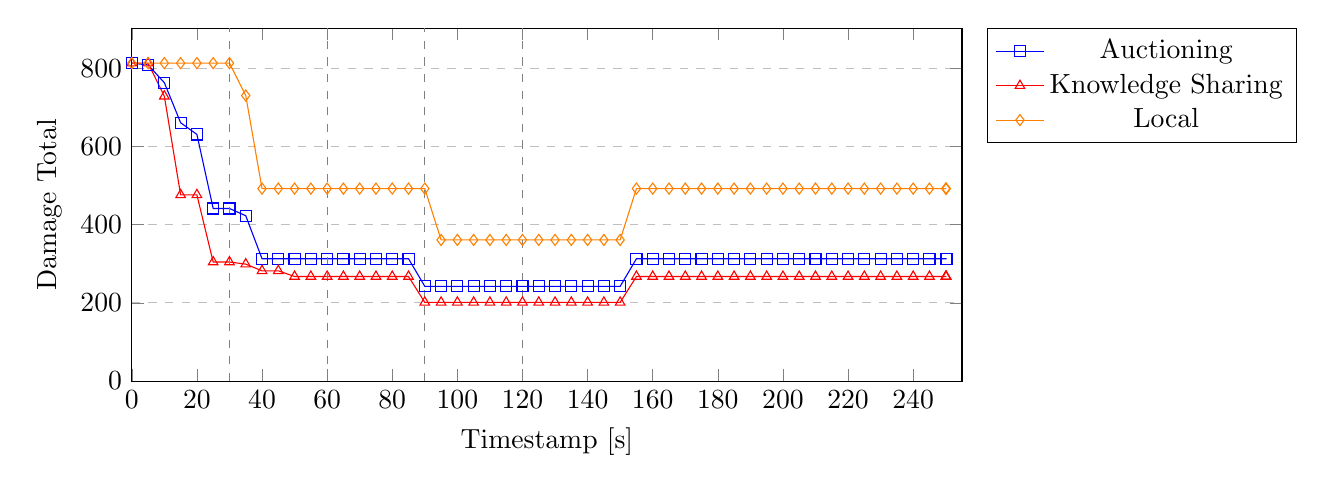
\begin{tikzpicture}
\begin{axis}[
    xlabel={Timestamp [s]},
    ylabel={Damage Total},
    xmin=0, xmax=255000,
    ymin=0, ymax=902,
    legend pos=outer north east,
    ymajorgrids=true,
    grid style=dashed,
    width=\textwidth,
    height=0.5\textwidth,
    scaled x ticks=base 10:-3,
    xtick scale label code/.code={}
]

	\addplot[color=blue,mark=square] coordinates {
        (0,812.71)(5000,808.17)(10000,762.80)(15000,660.38)(20000,630.54)(25000,441.18)(30000,441.18)(35000,422.77)(40000,312.76)(45000,312.76)(50000,312.76)(55000,312.76)(60000,312.76)(65000,312.76)(70000,312.76)(75000,312.76)(80000,312.76)(85000,312.76)(90000,242.13)(95000,242.13)(100000,242.13)(105000,242.13)(110000,242.13)(115000,242.13)(120000,242.13)(125000,242.13)(130000,242.13)(135000,242.13)(140000,242.13)(145000,242.13)(150000,242.13)(155000,312.76)(160000,312.76)(165000,312.76)(170000,312.76)(175000,312.76)(180000,312.76)(185000,312.76)(190000,312.76)(195000,312.76)(200000,312.76)(205000,312.76)(210000,312.76)(215000,312.76)(220000,312.76)(225000,312.76)(230000,312.76)(235000,312.76)(240000,312.76)(245000,312.76)(250000,312.76)(250270,312.76)
    };
    \addlegendentry{Auctioning}
	\addplot[color=red,mark=triangle] coordinates {
        (0,812.71)(5000,812.71)(10000,728.19)(15000,476.06)(20000,476.06)(25000,304.33)(30000,304.33)(35000,298.99)(40000,281.89)(45000,281.89)(50000,267.31)(55000,267.31)(60000,267.31)(65000,267.31)(70000,267.31)(75000,267.31)(80000,267.31)(85000,267.31)(90000,201.16)(95000,201.16)(100000,201.16)(105000,201.16)(110000,201.16)(115000,201.16)(120000,201.16)(125000,201.16)(130000,201.16)(135000,201.16)(140000,201.16)(145000,201.16)(150000,201.16)(155000,267.31)(160000,267.31)(165000,267.31)(170000,267.31)(175000,267.31)(180000,267.31)(185000,267.31)(190000,267.31)(195000,267.31)(200000,267.31)(205000,267.31)(210000,267.31)(215000,267.31)(220000,267.31)(225000,267.31)(230000,267.31)(235000,267.31)(240000,267.31)(245000,267.31)(250000,267.31)(250172,267.31)
    };
    \addlegendentry{Knowledge Sharing}
	\addplot[color=orange,mark=diamond] coordinates {
        (0,812.71)(5000,812.71)(10000,812.71)(15000,812.71)(20000,812.71)(25000,812.71)(30000,812.71)(35000,729.98)(40000,492.04)(45000,492.04)(50000,492.04)(55000,492.04)(60000,492.04)(65000,492.04)(70000,492.04)(75000,492.04)(80000,492.04)(85000,492.04)(90000,492.04)(95000,360.79)(100000,360.79)(105000,360.79)(110000,360.79)(115000,360.79)(120000,360.79)(125000,360.79)(130000,360.79)(135000,360.79)(140000,360.79)(145000,360.79)(150000,360.79)(155000,492.04)(160000,492.04)(165000,492.04)(170000,492.04)(175000,492.04)(180000,492.04)(185000,492.04)(190000,492.04)(195000,492.04)(200000,492.04)(205000,492.04)(210000,492.04)(215000,492.04)(220000,492.04)(225000,492.04)(230000,492.04)(235000,492.04)(240000,492.04)(245000,492.04)(250000,492.04)(250190,492.04)
    };
    \addlegendentry{Local}

	\addplot[color=gray, dashed,] coordinates {(30000,0) (30000,902)};
	\addplot[color=gray, dashed,] coordinates {(60000,0) (60000,902)};
	\addplot[color=gray, dashed,] coordinates {(90000,0) (90000,902)};
	\addplot[color=gray, dashed,] coordinates {(120000,0) (120000,902)};


\end{axis}
\end{tikzpicture}
    \caption{This graph shows the overall damage of the system in the unstable scenario. The damage is shown for each of the three strategies. The vertical lines indicate the time at which a node was removed and added again.}
    \label{fig:overall-damage-unstable}
\end{figure}

From this first Figure \ref{fig:overall-damage-unstable} we see a trend that is similar to the one from the first experiment (Figure \ref{fig:overall-damage-no-change}). The second time a node gets removed and then added, we see a small dip in the graphs. But apart from this there are no \emph{new} risks to mitigate as the properties of the nodes do not change. This is also reflected in Figure \ref{fig:messages-unstable}, where the knowledge-sharing agent does not see any property changes (and thus does not send any messages). The auctioning node does send some messages, as perviously due to the attempts of finding adaptations.

\begin{figure}[H]
    \centering
    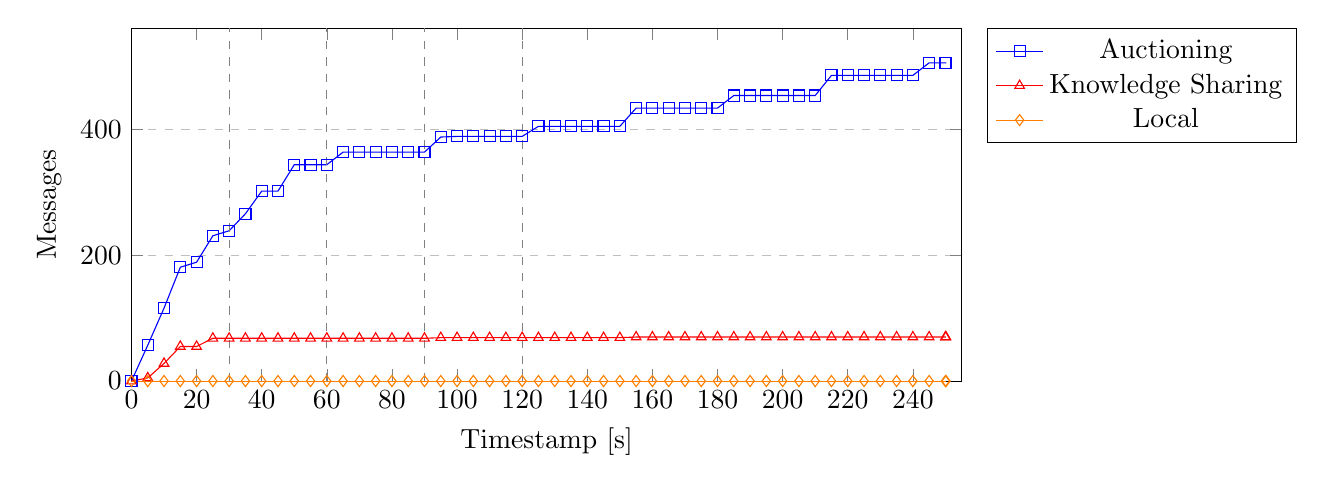
\begin{tikzpicture}
\begin{axis}[
    xlabel={Timestamp [s]},
    ylabel={Messages},
    xmin=0, xmax=255000,
    ymin=0, ymax=561,
    legend pos=outer north east,
    ymajorgrids=true,
    grid style=dashed,
    width=\textwidth,
    height=0.5\textwidth,
    scaled x ticks=base 10:-3,
    xtick scale label code/.code={}
]

	\addplot[color=blue,mark=square] coordinates {
        (0,0)(5000,57)(10000,116)(15000,181)(20000,189)(25000,231)(30000,239)(35000,266)(40000,302)(45000,302)(50000,344)(55000,344)(60000,344)(65000,364)(70000,364)(75000,364)(80000,364)(85000,364)(90000,364)(95000,388)(100000,389)(105000,389)(110000,389)(115000,389)(120000,389)(125000,405)(130000,405)(135000,405)(140000,405)(145000,405)(150000,405)(155000,434)(160000,434)(165000,434)(170000,434)(175000,434)(180000,434)(185000,454)(190000,454)(195000,454)(200000,454)(205000,454)(210000,454)(215000,486)(220000,486)(225000,486)(230000,486)(235000,486)(240000,486)(245000,506)(250000,506)(250270,506)
    };
    \addlegendentry{Auctioning}
	\addplot[color=red,mark=triangle] coordinates {
        (0,0)(5000,5)(10000,28)(15000,55)(20000,55)(25000,68)(30000,68)(35000,68)(40000,68)(45000,68)(50000,68)(55000,68)(60000,68)(65000,68)(70000,68)(75000,68)(80000,68)(85000,68)(90000,68)(95000,69)(100000,69)(105000,69)(110000,69)(115000,69)(120000,69)(125000,69)(130000,69)(135000,69)(140000,69)(145000,69)(150000,69)(155000,70)(160000,70)(165000,70)(170000,70)(175000,70)(180000,70)(185000,70)(190000,70)(195000,70)(200000,70)(205000,70)(210000,70)(215000,70)(220000,70)(225000,70)(230000,70)(235000,70)(240000,70)(245000,70)(250000,70)(250172,70)
    };
    \addlegendentry{Knowledge Sharing}
	\addplot[color=orange,mark=diamond] coordinates {
        (0,0)(5000,0)(10000,0)(15000,0)(20000,0)(25000,0)(30000,0)(35000,0)(40000,0)(45000,0)(50000,0)(55000,0)(60000,0)(65000,0)(70000,0)(75000,0)(80000,0)(85000,0)(90000,0)(95000,0)(100000,0)(105000,0)(110000,0)(115000,0)(120000,0)(125000,0)(130000,0)(135000,0)(140000,0)(145000,0)(150000,0)(155000,0)(160000,0)(165000,0)(170000,0)(175000,0)(180000,0)(185000,0)(190000,0)(195000,0)(200000,0)(205000,0)(210000,0)(215000,0)(220000,0)(225000,0)(230000,0)(235000,0)(240000,0)(245000,0)(250000,0)(250190,0)
    };
    \addlegendentry{Local}

	\addplot[color=gray, dashed,] coordinates {(30000,0) (30000,561)};
	\addplot[color=gray, dashed,] coordinates {(60000,0) (60000,561)};
	\addplot[color=gray, dashed,] coordinates {(90000,0) (90000,561)};
	\addplot[color=gray, dashed,] coordinates {(120000,0) (120000,561)};


\end{axis}
\end{tikzpicture}
    \caption{Graph showing the total amount of messages sent between agents in the unstable scenario.}
    \label{fig:messages-unstable}
\end{figure}

\begin{figure}[H]
    \centering
    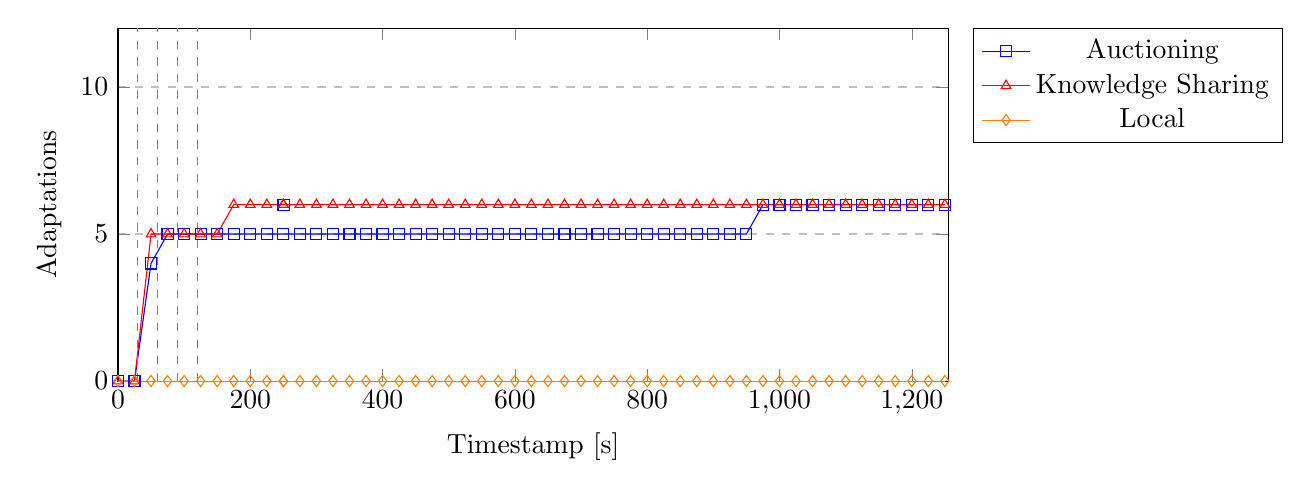
\begin{tikzpicture}
\begin{axis}[
    xlabel={Timestamp [s]},
    ylabel={Adaptations},
    xmin=0, xmax=1255000,
    ymin=0, ymax=12,
    legend pos=outer north east,
    ymajorgrids=true,
    grid style=dashed,
    width=\textwidth,
    height=0.5\textwidth,
    scaled x ticks=base 10:-3,
    xtick scale label code/.code={}
]

	\addplot[color=blue,mark=square] coordinates {
        (0,0)(25000,0)(50000,4)(75000,5)(100000,5)(125000,5)(150000,5)(175000,5)(200000,5)(225000,5)(250000,5)(275000,5)(300000,5)(325000,5)(350000,5)(375000,5)(400000,5)(425000,5)(450000,5)(475000,5)(500000,5)(525000,5)(550000,5)(575000,5)(600000,5)(625000,5)(650000,5)(675000,5)(700000,5)(725000,5)(750000,5)(775000,5)(800000,5)(825000,5)(850000,5)(875000,5)(900000,5)(925000,5)(950000,5)(975000,6)(1000000,6)(1025000,6)(1050000,6)(1075000,6)(1100000,6)(1125000,6)(1150000,6)(1175000,6)(1200000,6)(1225000,6)(1250000,6)(250362,6)
    };
    \addlegendentry{Auctioning}
	\addplot[color=red,mark=triangle] coordinates {
        (0,0)(25000,0)(50000,5)(75000,5)(100000,5)(125000,5)(150000,5)(175000,6)(200000,6)(225000,6)(250000,6)(275000,6)(300000,6)(325000,6)(350000,6)(375000,6)(400000,6)(425000,6)(450000,6)(475000,6)(500000,6)(525000,6)(550000,6)(575000,6)(600000,6)(625000,6)(650000,6)(675000,6)(700000,6)(725000,6)(750000,6)(775000,6)(800000,6)(825000,6)(850000,6)(875000,6)(900000,6)(925000,6)(950000,6)(975000,6)(1000000,6)(1025000,6)(1050000,6)(1075000,6)(1100000,6)(1125000,6)(1150000,6)(1175000,6)(1200000,6)(1225000,6)(1250000,6)(250334,6)
    };
    \addlegendentry{Knowledge Sharing}
	\addplot[color=orange,mark=diamond] coordinates {
        (0,0)(25000,0)(50000,0)(75000,0)(100000,0)(125000,0)(150000,0)(175000,0)(200000,0)(225000,0)(250000,0)(275000,0)(300000,0)(325000,0)(350000,0)(375000,0)(400000,0)(425000,0)(450000,0)(475000,0)(500000,0)(525000,0)(550000,0)(575000,0)(600000,0)(625000,0)(650000,0)(675000,0)(700000,0)(725000,0)(750000,0)(775000,0)(800000,0)(825000,0)(850000,0)(875000,0)(900000,0)(925000,0)(950000,0)(975000,0)(1000000,0)(1025000,0)(1050000,0)(1075000,0)(1100000,0)(1125000,0)(1150000,0)(1175000,0)(1200000,0)(1225000,0)(1250000,0)(250168,0)
    };
    \addlegendentry{Local}

	\addplot[color=gray, dashed,] coordinates {(30000,0) (30000,12)};
	\addplot[color=gray, dashed,] coordinates {(60000,0) (60000,12)};
	\addplot[color=gray, dashed,] coordinates {(90000,0) (90000,12)};
	\addplot[color=gray, dashed,] coordinates {(120000,0) (120000,12)};


\end{axis}
\end{tikzpicture}
    \caption{Graph showing the total amount of adaptations applied by agents in the unstable scenario.}
    \label{fig:proposals-unstable}
\end{figure}

Figure \ref{fig:proposals-unstable} is similar to the \emph{No change} scenario (Figure \ref{fig:proposals-no-change}), and is inline with the damage reduction visible in Figure \ref{fig:overall-damage-unstable}. No new adaptations are applied, and the infrastructure remains stable. The agents also do not detect any new risks, as the properties remain the same. This is reflected in Figure \ref{fig:risk-count-unstable} and \ref{fig:risk-remaining-unstable}.

\begin{figure}[H]
    \centering
        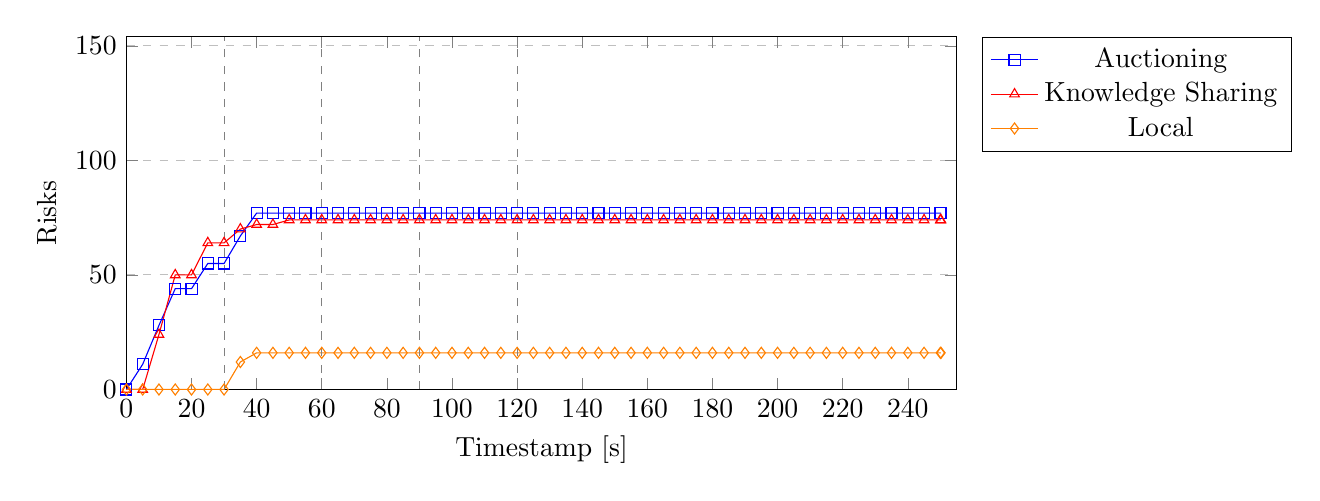
\begin{tikzpicture}
\begin{axis}[
    xlabel={Timestamp [s]},
    ylabel={Risks},
    xmin=0, xmax=255000,
    ymin=0, ymax=154,
    legend pos=outer north east,
    ymajorgrids=true,
    grid style=dashed,
    width=\textwidth,
    height=0.5\textwidth,
    scaled x ticks=base 10:-3,
    xtick scale label code/.code={}
]

	\addplot[color=blue,mark=square] coordinates {
        (0,0)(5000,11)(10000,28)(15000,44)(20000,44)(25000,55)(30000,55)(35000,67)(40000,77)(45000,77)(50000,77)(55000,77)(60000,77)(65000,77)(70000,77)(75000,77)(80000,77)(85000,77)(90000,77)(95000,77)(100000,77)(105000,77)(110000,77)(115000,77)(120000,77)(125000,77)(130000,77)(135000,77)(140000,77)(145000,77)(150000,77)(155000,77)(160000,77)(165000,77)(170000,77)(175000,77)(180000,77)(185000,77)(190000,77)(195000,77)(200000,77)(205000,77)(210000,77)(215000,77)(220000,77)(225000,77)(230000,77)(235000,77)(240000,77)(245000,77)(250000,77)(250270,77)
    };
    \addlegendentry{Auctioning}
	\addplot[color=red,mark=triangle] coordinates {
        (0,0)(5000,0)(10000,24)(15000,50)(20000,50)(25000,64)(30000,64)(35000,70)(40000,72)(45000,72)(50000,74)(55000,74)(60000,74)(65000,74)(70000,74)(75000,74)(80000,74)(85000,74)(90000,74)(95000,74)(100000,74)(105000,74)(110000,74)(115000,74)(120000,74)(125000,74)(130000,74)(135000,74)(140000,74)(145000,74)(150000,74)(155000,74)(160000,74)(165000,74)(170000,74)(175000,74)(180000,74)(185000,74)(190000,74)(195000,74)(200000,74)(205000,74)(210000,74)(215000,74)(220000,74)(225000,74)(230000,74)(235000,74)(240000,74)(245000,74)(250000,74)(250172,74)
    };
    \addlegendentry{Knowledge Sharing}
	\addplot[color=orange,mark=diamond] coordinates {
        (0,0)(5000,0)(10000,0)(15000,0)(20000,0)(25000,0)(30000,0)(35000,12)(40000,16)(45000,16)(50000,16)(55000,16)(60000,16)(65000,16)(70000,16)(75000,16)(80000,16)(85000,16)(90000,16)(95000,16)(100000,16)(105000,16)(110000,16)(115000,16)(120000,16)(125000,16)(130000,16)(135000,16)(140000,16)(145000,16)(150000,16)(155000,16)(160000,16)(165000,16)(170000,16)(175000,16)(180000,16)(185000,16)(190000,16)(195000,16)(200000,16)(205000,16)(210000,16)(215000,16)(220000,16)(225000,16)(230000,16)(235000,16)(240000,16)(245000,16)(250000,16)(250190,16)
    };
    \addlegendentry{Local}

	\addplot[color=gray, dashed,] coordinates {(30000,0) (30000,154)};
	\addplot[color=gray, dashed,] coordinates {(60000,0) (60000,154)};
	\addplot[color=gray, dashed,] coordinates {(90000,0) (90000,154)};
	\addplot[color=gray, dashed,] coordinates {(120000,0) (120000,154)};


\end{axis}
\end{tikzpicture}
    \caption{Graph showing the number of unique risks detected by agents in the unstable scenario.}
    \label{fig:risk-count-unstable}
\end{figure}

\begin{figure}[H]
    \centering
        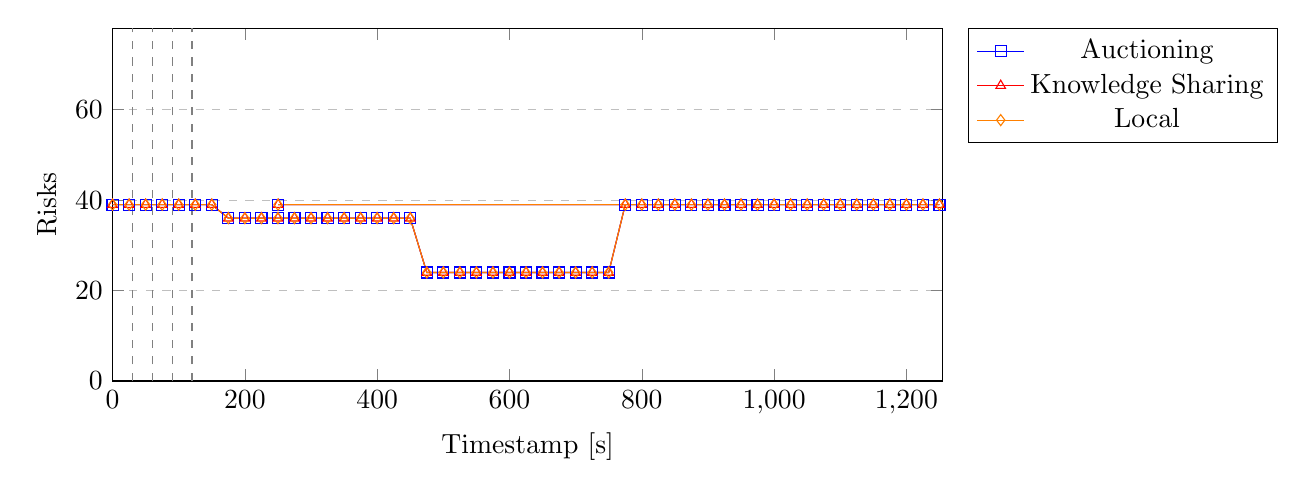
\begin{tikzpicture}
\begin{axis}[
    xlabel={Timestamp [s]},
    ylabel={Risks},
    xmin=0, xmax=1255000,
    ymin=0, ymax=78,
    legend pos=outer north east,
    ymajorgrids=true,
    grid style=dashed,
    width=\textwidth,
    height=0.5\textwidth,
    scaled x ticks=base 10:-3,
    xtick scale label code/.code={}
]

	\addplot[color=blue,mark=square] coordinates {
        (0,39)(25000,39)(50000,39)(75000,39)(100000,39)(125000,39)(150000,39)(175000,36)(200000,36)(225000,36)(250000,36)(275000,36)(300000,36)(325000,36)(350000,36)(375000,36)(400000,36)(425000,36)(450000,36)(475000,24)(500000,24)(525000,24)(550000,24)(575000,24)(600000,24)(625000,24)(650000,24)(675000,24)(700000,24)(725000,24)(750000,24)(775000,39)(800000,39)(825000,39)(850000,39)(875000,39)(900000,39)(925000,39)(950000,39)(975000,39)(1000000,39)(1025000,39)(1050000,39)(1075000,39)(1100000,39)(1125000,39)(1150000,39)(1175000,39)(1200000,39)(1225000,39)(1250000,39)(250362,39)
    };
    \addlegendentry{Auctioning}
	\addplot[color=red,mark=triangle] coordinates {
        (0,39)(25000,39)(50000,39)(75000,39)(100000,39)(125000,39)(150000,39)(175000,36)(200000,36)(225000,36)(250000,36)(275000,36)(300000,36)(325000,36)(350000,36)(375000,36)(400000,36)(425000,36)(450000,36)(475000,24)(500000,24)(525000,24)(550000,24)(575000,24)(600000,24)(625000,24)(650000,24)(675000,24)(700000,24)(725000,24)(750000,24)(775000,39)(800000,39)(825000,39)(850000,39)(875000,39)(900000,39)(925000,39)(950000,39)(975000,39)(1000000,39)(1025000,39)(1050000,39)(1075000,39)(1100000,39)(1125000,39)(1150000,39)(1175000,39)(1200000,39)(1225000,39)(1250000,39)(250334,39)
    };
    \addlegendentry{Knowledge Sharing}
	\addplot[color=orange,mark=diamond] coordinates {
        (0,39)(25000,39)(50000,39)(75000,39)(100000,39)(125000,39)(150000,39)(175000,36)(200000,36)(225000,36)(250000,36)(275000,36)(300000,36)(325000,36)(350000,36)(375000,36)(400000,36)(425000,36)(450000,36)(475000,24)(500000,24)(525000,24)(550000,24)(575000,24)(600000,24)(625000,24)(650000,24)(675000,24)(700000,24)(725000,24)(750000,24)(775000,39)(800000,39)(825000,39)(850000,39)(875000,39)(900000,39)(925000,39)(950000,39)(975000,39)(1000000,39)(1025000,39)(1050000,39)(1075000,39)(1100000,39)(1125000,39)(1150000,39)(1175000,39)(1200000,39)(1225000,39)(1250000,39)(250168,39)
    };
    \addlegendentry{Local}

	\addplot[color=gray, dashed,] coordinates {(30000,0) (30000,78)};
	\addplot[color=gray, dashed,] coordinates {(60000,0) (60000,78)};
	\addplot[color=gray, dashed,] coordinates {(90000,0) (90000,78)};
	\addplot[color=gray, dashed,] coordinates {(120000,0) (120000,78)};


\end{axis}
\end{tikzpicture}
    \caption{Graph showing the number of remaining risks in the infrastructure in the unstable scenario.}
    \label{fig:risk-remaining-unstable}
\end{figure}

\add{write}

\begin{figure}[H]
    \hspace*{-1cm}
    \centering
        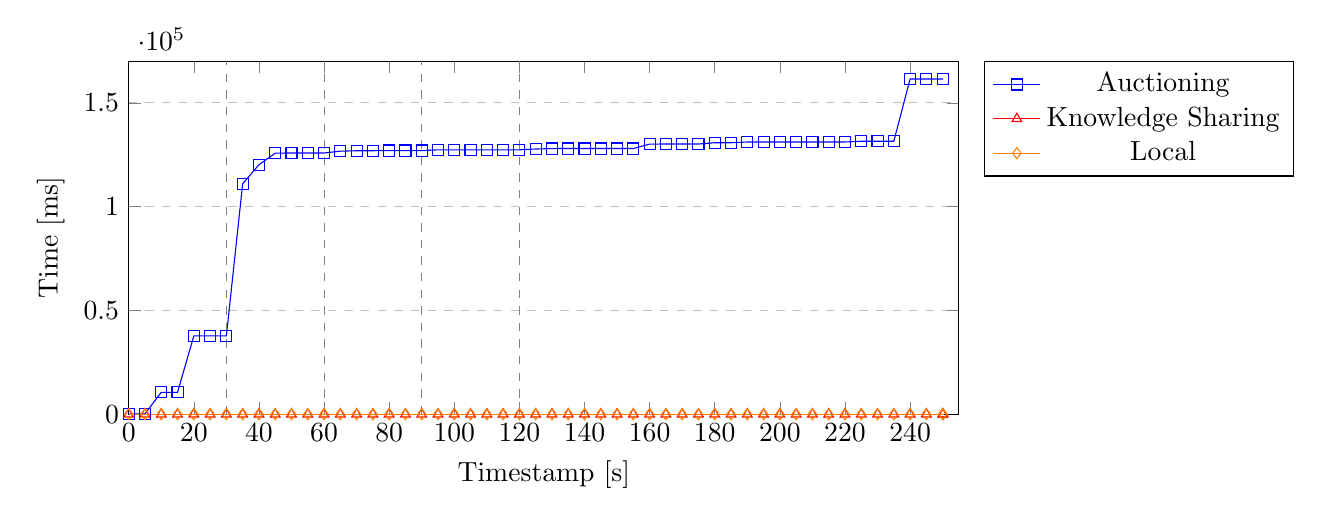
\begin{tikzpicture}
\begin{axis}[
    xlabel={Timestamp [s]},
    ylabel={Time [ms]},
    xmin=0, xmax=255000,
    ymin=0, ymax=170017,
    legend pos=outer north east,
    ymajorgrids=true,
    grid style=dashed,
    width=\textwidth,
    height=0.5\textwidth,
    scaled x ticks=base 10:-3,
    xtick scale label code/.code={}
]

	\addplot[color=blue,mark=square] coordinates {
        (0,0)(5000,173)(10000,10538)(15000,10538)(20000,37730)(25000,37730)(30000,37730)(35000,111030)(40000,120177)(45000,125786)(50000,125855)(55000,125855)(60000,125855)(65000,126731)(70000,126932)(75000,126952)(80000,127013)(85000,127013)(90000,127013)(95000,127365)(100000,127365)(105000,127385)(110000,127385)(115000,127385)(120000,127385)(125000,127764)(130000,127985)(135000,128006)(140000,128006)(145000,128006)(150000,128006)(155000,128006)(160000,130144)(165000,130172)(170000,130172)(175000,130172)(180000,130795)(185000,130795)(190000,131135)(195000,131135)(200000,131161)(205000,131161)(210000,131161)(215000,131161)(220000,131161)(225000,131489)(230000,131517)(235000,131517)(240000,161517)(245000,161517)(250000,161517)(250144,161517)
    };
    \addlegendentry{Auctioning}
	\addplot[color=red,mark=triangle] coordinates {
        (0,0)(5000,0)(10000,0)(15000,0)(20000,0)(25000,0)(30000,0)(35000,0)(40000,0)(45000,0)(50000,0)(55000,0)(60000,0)(65000,0)(70000,0)(75000,0)(80000,0)(85000,0)(90000,0)(95000,0)(100000,0)(105000,0)(110000,0)(115000,0)(120000,0)(125000,0)(130000,0)(135000,0)(140000,0)(145000,0)(150000,0)(155000,0)(160000,0)(165000,0)(170000,0)(175000,0)(180000,0)(185000,0)(190000,0)(195000,0)(200000,0)(205000,0)(210000,0)(215000,0)(220000,0)(225000,0)(230000,0)(235000,0)(240000,0)(245000,0)(250000,0)(250118,0)
    };
    \addlegendentry{Knowledge Sharing}
	\addplot[color=orange,mark=diamond] coordinates {
        (0,0)(5000,0)(10000,0)(15000,0)(20000,0)(25000,0)(30000,0)(35000,0)(40000,0)(45000,0)(50000,0)(55000,0)(60000,0)(65000,0)(70000,0)(75000,0)(80000,0)(85000,0)(90000,0)(95000,0)(100000,0)(105000,0)(110000,0)(115000,0)(120000,0)(125000,0)(130000,0)(135000,0)(140000,0)(145000,0)(150000,0)(155000,0)(160000,0)(165000,0)(170000,0)(175000,0)(180000,0)(185000,0)(190000,0)(195000,0)(200000,0)(205000,0)(210000,0)(215000,0)(220000,0)(225000,0)(230000,0)(235000,0)(240000,0)(245000,0)(250000,0)(250091,0)
    };
    \addlegendentry{Local}

	\addplot[color=gray, dashed,] coordinates {(30000,0) (30000,170017)};
	\addplot[color=gray, dashed,] coordinates {(60000,0) (60000,170017)};
	\addplot[color=gray, dashed,] coordinates {(90000,0) (90000,170017)};
	\addplot[color=gray, dashed,] coordinates {(120000,0) (120000,170017)};


\end{axis}
\end{tikzpicture}
    \caption{Graph showing the sum of time spent auctioning by agents in the unstable scenario.}
    \label{fig:auctioning-time-unstable}
\end{figure}

\begin{figure}[H]
    \hspace*{-1cm}
    \centering
        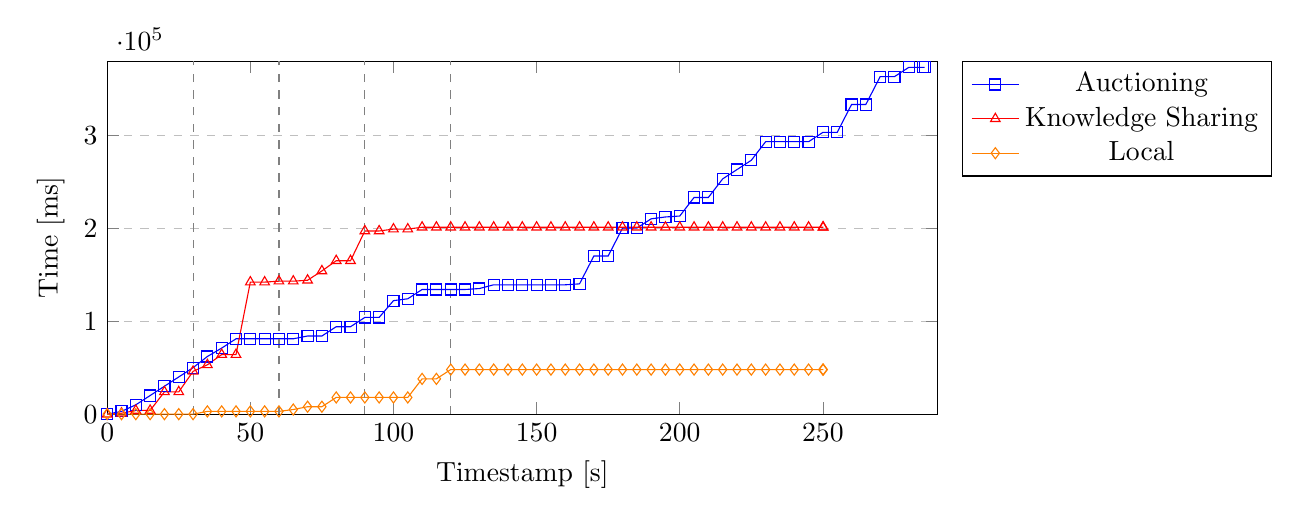
\begin{tikzpicture}
\begin{axis}[
    xlabel={Timestamp [s]},
    ylabel={Time [ms]},
    xmin=0, xmax=290000,
    ymin=0, ymax=380038,
    legend pos=outer north east,
    ymajorgrids=true,
    grid style=dashed,
    width=\textwidth,
    height=0.5\textwidth,
    scaled x ticks=base 10:-3,
    xtick scale label code/.code={}
]

	\addplot[color=blue,mark=square] coordinates {
        (0,0)(5000,3015)(10000,10073)(15000,20083)(20000,30092)(25000,40100)(30000,50105)(35000,62134)(40000,71193)(45000,81199)(50000,81199)(55000,81199)(60000,81199)(65000,81199)(70000,84209)(75000,84209)(80000,94219)(85000,94219)(90000,104222)(95000,104222)(100000,122281)(105000,124295)(110000,134306)(115000,134306)(120000,134306)(125000,134306)(130000,135314)(135000,139351)(140000,139351)(145000,139351)(150000,139351)(155000,139351)(160000,139351)(165000,140360)(170000,170377)(175000,170377)(180000,200396)(185000,200396)(190000,210405)(195000,212415)(200000,213423)(205000,233437)(210000,233437)(215000,253455)(220000,263466)(225000,273475)(230000,293490)(235000,293490)(240000,293490)(245000,293490)(250000,303496)(255000,303496)(260000,333521)(265000,333521)(270000,363542)(275000,363542)(280000,373547)(285000,373547)(285530,373547)
    };
    \addlegendentry{Auctioning}
	\addplot[color=red,mark=triangle] coordinates {
        (0,0)(5000,1009)(10000,4030)(15000,4030)(20000,24044)(25000,24044)(30000,46078)(35000,53188)(40000,64205)(45000,64205)(50000,142255)(55000,142255)(60000,143258)(65000,143258)(70000,144266)(75000,154274)(80000,165289)(85000,165289)(90000,197316)(95000,197316)(100000,199335)(105000,199335)(110000,201346)(115000,201346)(120000,201346)(125000,201346)(130000,201346)(135000,201346)(140000,201346)(145000,201346)(150000,201346)(155000,201346)(160000,201346)(165000,201346)(170000,201346)(175000,201346)(180000,201346)(185000,201346)(190000,201346)(195000,201346)(200000,201346)(205000,201346)(210000,201346)(215000,201346)(220000,201346)(225000,201346)(230000,201346)(235000,201346)(240000,201346)(245000,201346)(250000,201346)(250138,201346)
    };
    \addlegendentry{Knowledge Sharing}
	\addplot[color=orange,mark=diamond] coordinates {
        (0,0)(5000,0)(10000,0)(15000,0)(20000,0)(25000,0)(30000,0)(35000,3011)(40000,3011)(45000,3011)(50000,3011)(55000,3011)(60000,3011)(65000,5019)(70000,8033)(75000,8033)(80000,18038)(85000,18038)(90000,18038)(95000,18038)(100000,18038)(105000,18038)(110000,38043)(115000,38043)(120000,48045)(125000,48045)(130000,48045)(135000,48045)(140000,48045)(145000,48045)(150000,48045)(155000,48045)(160000,48045)(165000,48045)(170000,48045)(175000,48045)(180000,48045)(185000,48045)(190000,48045)(195000,48045)(200000,48045)(205000,48045)(210000,48045)(215000,48045)(220000,48045)(225000,48045)(230000,48045)(235000,48045)(240000,48045)(245000,48045)(250000,48045)(250134,48045)
    };
    \addlegendentry{Local}

	\addplot[color=gray, dashed,] coordinates {(30000,0) (30000,380038)};
	\addplot[color=gray, dashed,] coordinates {(60000,0) (60000,380038)};
	\addplot[color=gray, dashed,] coordinates {(90000,0) (90000,380038)};
	\addplot[color=gray, dashed,] coordinates {(120000,0) (120000,380038)};


\end{axis}
\end{tikzpicture}
    \caption{Graph showing the sum of time spent adapting by agents in the unstable scenario.}
    \label{fig:adapting-time-unstable}
\end{figure}

As with the prior graphs for this scenario we see that Figure \ref{fig:adapting-time-unstable} is also stable after the first $50$ seconds. There are no new risks as shown in Figure \ref{fig:risk-count-unstable} and no new adaptations are necessary to mitigate them. 



\subsection*{Consecutive runs}
\begin{figure}[H]
    \centering
        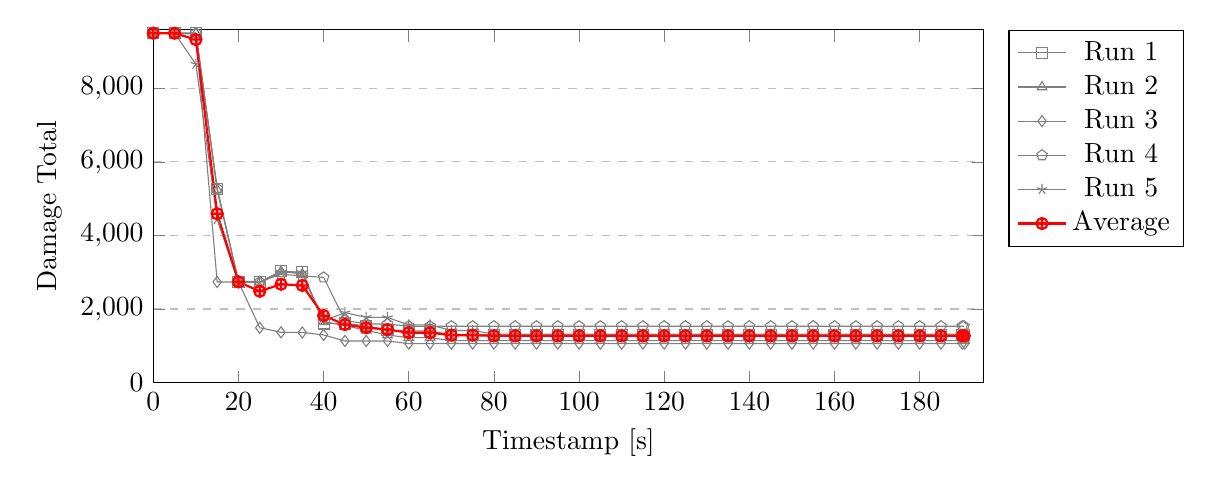
\begin{tikzpicture}
\begin{axis}[
    xlabel={Timestamp [s]},
    ylabel={Damage Total},
    xmin=0, xmax=195000,
    ymin=0, ymax=9595,
    legend pos=outer north east,
    ymajorgrids=true,
    grid style=dashed,
    width=\textwidth,
    height=0.5\textwidth,
    scaled x ticks=base 10:-3,
    xtick scale label code/.code={}
]

	\addplot[color=gray,mark=square] coordinates {
        (0,9500.86)(5000,9500.86)(10000,9500.86)(15000,5273.46)(20000,2735.67)(25000,2733.78)(30000,3030.23)(35000,2999.27)(40000,1606.26)(45000,1606.26)(50000,1545.84)(55000,1424.29)(60000,1401.35)(65000,1401.35)(70000,1299.55)(75000,1299.55)(80000,1299.55)(85000,1299.55)(90000,1299.55)(95000,1299.55)(100000,1299.55)(105000,1299.55)(110000,1299.55)(115000,1299.55)(120000,1299.55)(125000,1299.55)(130000,1299.55)(135000,1299.55)(140000,1299.55)(145000,1299.55)(150000,1299.55)(155000,1299.55)(160000,1299.55)(165000,1299.55)(170000,1299.55)(175000,1299.55)(180000,1299.55)(185000,1299.55)(190000,1299.55)(190469,1299.55)
    };
    \addlegendentry{Run 1}
	\addplot[color=gray,mark=triangle] coordinates {
        (0,9500.86)(5000,9500.86)(10000,9500.86)(15000,5244.51)(20000,2735.67)(25000,2733.78)(30000,3027.26)(35000,2951.72)(40000,1657.47)(45000,1550.25)(50000,1420.21)(55000,1293.76)(60000,1220.39)(65000,1220.39)(70000,1142.59)(75000,1142.59)(80000,1142.59)(85000,1142.59)(90000,1142.59)(95000,1142.59)(100000,1142.59)(105000,1142.59)(110000,1142.59)(115000,1142.59)(120000,1142.59)(125000,1142.59)(130000,1142.59)(135000,1142.59)(140000,1142.59)(145000,1142.59)(150000,1142.59)(155000,1142.59)(160000,1142.59)(165000,1142.59)(170000,1142.59)(175000,1142.59)(180000,1142.59)(185000,1142.59)(190000,1142.59)(190603,1142.59)
    };
    \addlegendentry{Run 2}
	\addplot[color=gray,mark=diamond] coordinates {
        (0,9500.86)(5000,9500.86)(10000,9475.27)(15000,2735.67)(20000,2735.67)(25000,1491.74)(30000,1368.06)(35000,1362.13)(40000,1296.28)(45000,1131.00)(50000,1131.00)(55000,1131.00)(60000,1059.17)(65000,1059.17)(70000,1059.17)(75000,1059.17)(80000,1059.17)(85000,1059.17)(90000,1059.17)(95000,1059.17)(100000,1059.17)(105000,1059.17)(110000,1059.17)(115000,1059.17)(120000,1059.17)(125000,1059.17)(130000,1059.17)(135000,1059.17)(140000,1059.17)(145000,1059.17)(150000,1059.17)(155000,1059.17)(160000,1059.17)(165000,1059.17)(170000,1059.17)(175000,1059.17)(180000,1059.17)(185000,1059.17)(190000,1059.17)(190583,1059.17)
    };
    \addlegendentry{Run 3}
	\addplot[color=gray,mark=pentagon] coordinates {
        (0,9500.86)(5000,9500.86)(10000,9500.86)(15000,5273.46)(20000,2757.80)(25000,2735.67)(30000,2946.76)(35000,2901.60)(40000,2859.47)(45000,1695.56)(50000,1592.95)(55000,1592.95)(60000,1531.57)(65000,1531.57)(70000,1531.57)(75000,1531.57)(80000,1531.57)(85000,1531.57)(90000,1531.57)(95000,1531.57)(100000,1531.57)(105000,1531.57)(110000,1531.57)(115000,1531.57)(120000,1531.57)(125000,1531.57)(130000,1531.57)(135000,1531.57)(140000,1531.57)(145000,1531.57)(150000,1531.57)(155000,1531.57)(160000,1531.57)(165000,1531.57)(170000,1531.57)(175000,1531.57)(180000,1531.57)(185000,1531.57)(190000,1531.57)(190405,1531.57)
    };
    \addlegendentry{Run 4}
	\addplot[color=gray,mark=star] coordinates {
        (0,9500.86)(5000,9500.86)(10000,8658.83)(15000,4434.90)(20000,2726.22)(25000,2726.22)(30000,3000.82)(35000,2997.05)(40000,1685.04)(45000,1899.99)(50000,1777.19)(55000,1769.17)(60000,1569.23)(65000,1569.23)(70000,1417.12)(75000,1417.12)(80000,1318.25)(85000,1318.25)(90000,1318.25)(95000,1318.25)(100000,1318.25)(105000,1318.25)(110000,1318.25)(115000,1318.25)(120000,1318.25)(125000,1318.25)(130000,1318.25)(135000,1318.25)(140000,1318.25)(145000,1318.25)(150000,1318.25)(155000,1318.25)(160000,1318.25)(165000,1318.25)(170000,1318.25)(175000,1318.25)(180000,1318.25)(185000,1318.25)(190000,1318.25)(190567,1318.25)
    };
    \addlegendentry{Run 5}
	\addplot[color=red,mark=oplus,thick] coordinates {
        (0,9500)(5000,9500)(10000,9326.6)(15000,4591.8)(20000,2737.6)(25000,2483.6)(30000,2674.2)(35000,2642)(40000,1820.6)(45000,1576.2)(50000,1493)(55000,1441.8)(60000,1356)(65000,1356)(70000,1289.6)(75000,1289.6)(80000,1269.8)(85000,1269.8)(90000,1269.8)(95000,1269.8)(100000,1269.8)(105000,1269.8)(110000,1269.8)(115000,1269.8)(120000,1269.8)(125000,1269.8)(130000,1269.8)(135000,1269.8)(140000,1269.8)(145000,1269.8)(150000,1269.8)(155000,1269.8)(160000,1269.8)(165000,1269.8)(170000,1269.8)(175000,1269.8)(180000,1269.8)(185000,1269.8)(190000,1269.8)(190469,1269.8)
    };
    \addlegendentry{Average}
\end{axis}
\end{tikzpicture}

    \caption{Graph showing the Auctioning Feature's performance over multiple runs in the no-change scenario.}
\end{figure}

\subsection*{Small Infrastructure}
\begin{figure}[H]
    \centering
        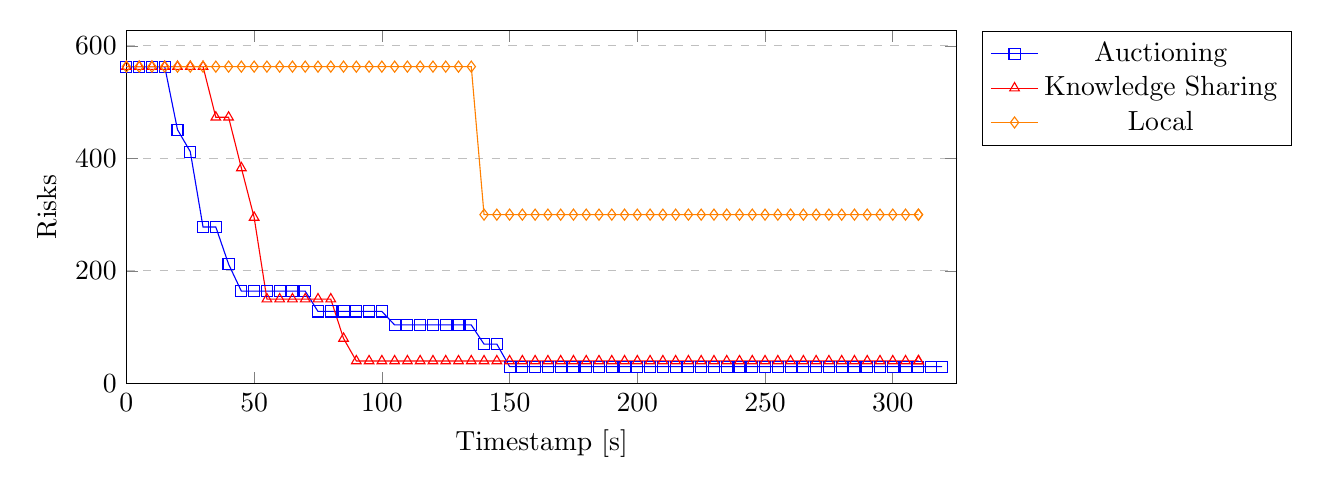
\begin{tikzpicture}
\begin{axis}[
    xlabel={Timestamp [s]},
    ylabel={Risks},
    xmin=0, xmax=325000,
    ymin=0, ymax=627,
    legend pos=outer north east,
    ymajorgrids=true,
    grid style=dashed,
    width=\textwidth,
    height=0.5\textwidth,
    scaled x ticks=base 10:-3,
    xtick scale label code/.code={}
]

	\addplot[color=blue,mark=square] coordinates {
        (0,563)(5000,563)(10000,563)(15000,563)(20000,451)(25000,412)(30000,278)(35000,278)(40000,212)(45000,164)(50000,164)(55000,164)(60000,164)(65000,164)(70000,164)(75000,128)(80000,128)(85000,128)(90000,128)(95000,128)(100000,128)(105000,104)(110000,104)(115000,104)(120000,104)(125000,104)(130000,104)(135000,104)(140000,70)(145000,70)(150000,30)(155000,30)(160000,30)(165000,30)(170000,30)(175000,30)(180000,30)(185000,30)(190000,30)(195000,30)(200000,30)(205000,30)(210000,30)(215000,30)(220000,30)(225000,30)(230000,30)(235000,30)(240000,30)(245000,30)(250000,30)(255000,30)(260000,30)(265000,30)(270000,30)(275000,30)(280000,30)(285000,30)(290000,30)(295000,30)(300000,30)(305000,30)(310000,30)(315000,30)(319272,30)
    };
    \addlegendentry{Auctioning}
	\addplot[color=red,mark=triangle] coordinates {
        (0,563)(5000,563)(10000,563)(15000,563)(20000,563)(25000,563)(30000,563)(35000,473)(40000,473)(45000,383)(50000,295)(55000,150)(60000,150)(65000,150)(70000,150)(75000,150)(80000,150)(85000,80)(90000,40)(95000,40)(100000,40)(105000,40)(110000,40)(115000,40)(120000,40)(125000,40)(130000,40)(135000,40)(140000,40)(145000,40)(150000,40)(155000,40)(160000,40)(165000,40)(170000,40)(175000,40)(180000,40)(185000,40)(190000,40)(195000,40)(200000,40)(205000,40)(210000,40)(215000,40)(220000,40)(225000,40)(230000,40)(235000,40)(240000,40)(245000,40)(250000,40)(255000,40)(260000,40)(265000,40)(270000,40)(275000,40)(280000,40)(285000,40)(290000,40)(295000,40)(300000,40)(305000,40)(310000,40)(310115,40)
    };
    \addlegendentry{Knowledge Sharing}
	\addplot[color=orange,mark=diamond] coordinates {
        (0,563)(5000,563)(10000,563)(15000,563)(20000,563)(25000,563)(30000,563)(35000,563)(40000,563)(45000,563)(50000,563)(55000,563)(60000,563)(65000,563)(70000,563)(75000,563)(80000,563)(85000,563)(90000,563)(95000,563)(100000,563)(105000,563)(110000,563)(115000,563)(120000,563)(125000,563)(130000,563)(135000,563)(140000,300)(145000,300)(150000,300)(155000,300)(160000,300)(165000,300)(170000,300)(175000,300)(180000,300)(185000,300)(190000,300)(195000,300)(200000,300)(205000,300)(210000,300)(215000,300)(220000,300)(225000,300)(230000,300)(235000,300)(240000,300)(245000,300)(250000,300)(255000,300)(260000,300)(265000,300)(270000,300)(275000,300)(280000,300)(285000,300)(290000,300)(295000,300)(300000,300)(305000,300)(310000,300)(310098,300)
    };
    \addlegendentry{Local}




\end{axis}
\end{tikzpicture}
    \caption{Graph showing the output of all feature sets in the non-changing scenario, with a small infrastructure.}
\end{figure}
 

\section{Discussion}
\label{sec:discussion}

\add{Mention how the results can be interpreted}
\add{Relate this to the research questions}

\add{Mention the performance of knowledge-sharing in smaller networks}
\add{Mention the effects of compromised agents and the impact}

\section{Future Research}
\label{sec:future-research}

\begin{itemize}
    \item More complex risk rules.
    \item Different Depths for messages.
    \item Simplifying the riskreport sent in the auction.
\end{itemize}

\section{Conclusion}
\label{sec:conclusion}


\add{Relate discussion to the research questions}


\bibliographystyle{abbrv}
\bibliography{bibliography}
\end{document}
